\documentclass[11pt,a4paper]{article}
\usepackage{fontspec}
\usepackage[spanish,es-noshorthands]{babel}
\usepackage{amsmath,amssymb,mathtools}
\usepackage[a4paper,margin=2.7cm]{geometry}
\usepackage{booktabs,array,longtable}
\newcolumntype{L}[1]{>{\raggedright\arraybackslash}p{#1}}
\usepackage[dvipsnames]{xcolor}
\usepackage{graphicx}
\usepackage{enumitem}
\usepackage{microtype}
\usepackage{fancyhdr}
\usepackage[most]{tcolorbox}
\usepackage[font=small,labelfont=bf,labelsep=period]{caption}
\usepackage{titlesec}
\usepackage[colorlinks=true,linkcolor=NavyBlue,citecolor=NavyBlue,urlcolor=NavyBlue]{hyperref}

\numberwithin{equation}{section}
\allowdisplaybreaks
\setlength{\parindent}{1.3em}
\setlength{\parskip}{0.25em}
\linespread{1.1}

\pagestyle{fancy}
\fancyhf{}
\fancyhead[L]{\small\color{gray}Gravedad unimodular, inflación y ondas gravitacionales primordiales}
\fancyhead[R]{\small\color{gray}\thepage}
\renewcommand{\headrulewidth}{0.3pt}
\titleformat{\section}{\Large\bfseries\color{NavyBlue}}{\thesection}{0.7em}{}
\titleformat{\subsection}{\large\bfseries}{\thesubsection}{0.6em}{}
\titleformat{\subsubsection}{\normalsize\bfseries\itshape}{\thesubsubsection}{0.6em}{}
\titlespacing*{\section}{0pt}{2.0em}{0.8em}

% ---- símbolos
\newcommand{\MP}{M_{\rm P}}
\newcommand{\kap}{\kappa}
\newcommand{\Lb}{\bar\lambda}
\newcommand{\dd}{\mathrm d}
\newcommand{\ee}{\mathrm e}
\newcommand{\PT}{P_T}
% permitir cortes de línea después de los guiones bajos (nombres de funciones en \texttt)
\let\oldunderscore\_
\renewcommand{\_}{\oldunderscore\hspace{0pt}}
% etiqueta de procedencia: [P] propia, [C] citada, [E] estándar, [S] supuesto
\newcommand{\etq}[1]{\,{\footnotesize\color{gray}[#1]}}

% ---- cajas
\tcbset{cajabase/.style={breakable,enhanced,boxrule=0.6pt,arc=2pt,left=8pt,right=8pt,top=5pt,bottom=5pt,before skip=9pt,after skip=9pt,fonttitle=\bfseries\small}}
\newtcolorbox{idea}[1][Idea]{cajabase,colback=NavyBlue!5,colframe=NavyBlue!65,title={#1}}
\newtcolorbox{alerta}[1][Advertencia]{cajabase,colback=BurntOrange!8,colframe=BurntOrange!80,title={#1}}
\newtcolorbox{resultado}[1][Resultado]{cajabase,colback=OliveGreen!7,colframe=OliveGreen!70,title={#1}}

\graphicspath{{../codigo/figuras/}}

\title{\textbf{Gravedad unimodular, inflación\\ y ondas gravitacionales primordiales}\\[0.6em]
\large Informe de trabajo: fundamentos, derivación del sector tensorial con difusión\\ y cálculo numérico de $P_T(k)$}
\author{Javier Pineau\\ \small Curso GW IA --- Entrega final}
\date{28 de septiembre de 2026}

\begin{document}
\maketitle
\thispagestyle{fancy}

\begin{abstract}
\noindent
Este informe reúne, en un texto continuo, el trabajo sobre el espectro de potencia tensorial primordial en gravedad unimodular (UG) con difusión $Q$, comparado con relatividad general (RG). Parte de lo elemental (relatividad general, cosmología homogénea, inflación y su espectro tensorial en RG), presenta la gravedad unimodular y el término de difusión que aparece cuando se permite que la energía-impulso no se conserve, y desarrolla la derivación analítica y el cálculo numérico. El resultado analítico central es que, sobre un fondo homogéneo y bajo la hipótesis de que la materia no aporta tensión anisótropa TT, la ecuación de los modos tensoriales y su acción cuadrática (esta última como hipótesis de la realización efectiva, que fija la normalización cuántica) son idénticas a las de RG: el vínculo unimodular no actúa sobre los modos transversos y sin traza a primer orden, y a segundo orden su contribución se cancela con las del resto de la acción, de modo que $Q$ entra en el espectro solamente a través de $H(t)$. La ecuación a primer orden se verificó con álgebra simbólica. El cálculo numérico se hizo para un inflatón con dos potenciales, el cuadrático y el de Starobinsky, y $Q(N)=Q_i\ee^{-\gamma N}$. A igual $k$ comóvil, UG suprime el espectro tensorial en el cuadrático (de $0.914$ a $0.344$ frente a RG), pero esa conclusión \emph{no es robusta}: al comparar a igual número de e-folds antes del final de cada inflación el cociente es $1.5$ (UG aumenta), y con Starobinsky es $\approx0.90$ a igual $N_*$ y $0.947$--$0.796$ a igual $k$. Los controles numéricos atribuyen la diferencia a la evolución distinta del fondo. Se muestra además que para un escalar canónico con la difusión especificada como ley local $Q(\phi)$ las ecuaciones de UG son las de RG con un potencial efectivo $V_{\rm eff}=V+Q(\phi)+\Lambda_0$ (con las salvedades de la sección~\ref{sec:unescalar}: no es una equivalencia irrestricta de teorías), y que imponer $\delta Q=0$ en el marco indicado, con perturbaciones inhomogéneas del inflatón, exige $\dot Q=0$; el alcance a otros gauges y a perturbaciones uniformes no se analizó. Con el modelo de radiación con difusión Q \cite{leon22,piccirilli23} (radiación pura más $Q$, sin inflatón, $\delta Q=0$) el espectro tensorial es el de RG con el mismo $H(N)$ (coinciden a $\sim10^{-6}$), y se calcula para los escenarios de reconstrucción de la literatura del grupo; $A_s$ sale $1.1\%$ por encima de Planck en su punto de referencia, sin ajustar nada, con la fórmula escalar de \cite{piccirilli23}, y cinco veces mayor con la de \cite{leon22} (normalización de esa referencia, no reajustada). El informe discute de qué decisiones depende la magnitud (en particular, $\Lambda_0$ y el criterio de comparación), qué supuestos sobre la materia sostienen el resultado analítico, y qué queda abierto, empezando por el sector escalar en el marco $\delta Q=0$. Está pensado para leerse de corrido y para decidir, con los desarrollos a la vista, si se está de acuerdo con las conclusiones.
\end{abstract}

\vspace{0.5em}
\begin{alerta}[Cómo leer este informe]
Cada resultado importante lleva una etiqueta entre corchetes que indica su procedencia: \etq{P} álgebra propia, hecha a mano en este trabajo; \etq{C} resultado tomado de un artículo, con su referencia; \etq{E} resultado estándar de libro de texto, usado tal cual; \etq{S} supuesto o decisión de modelado. Los resultados propios se verificaron a mano y, cuando corresponde, con los controles numéricos de la sección~\ref{sec:resultados}; \textbf{solo se verificaron con álgebra simbólica por computadora, a primer orden, los pasos que la sección~\ref{sec:acoplamiento} indica} (la acción a segundo orden no), y varias referencias solo se leyeron en parte (Apéndice~\ref{ap:fuentes}). La tabla del Apéndice~\ref{ap:procedencia} enlaza cada ecuación clave con su lugar en el código y en los archivos de derivación del proyecto. El resumen de qué se puede afirmar y qué no está en la sección~\ref{sec:discusion}.
\end{alerta}

\tableofcontents
\clearpage

\section{Introducción}
\label{sec:intro}

La inflación cósmica predice que, además de las fluctuaciones de densidad que sembraron las galaxias, el universo primitivo generó un fondo de ondas gravitacionales. Su amplitud está fijada por la escala de energía a la que ocurrió la inflación: en relatividad general (RG), el espectro de potencia de esas ondas vale, a orden más bajo, $2H^2/(\pi^2\MP^2)$ evaluado en el momento en que cada modo sale del horizonte, donde $H$ es el parámetro de Hubble y $\MP$ la masa de Planck reducida. Por eso el espectro tensorial primordial es una de las pocas ventanas observacionales hacia la física de la inflación, y por eso las cotas actuales sobre la relación tensor-escalar $r$ (Planck, BICEP/Keck) restringen tanto los modelos.

La gravedad unimodular (UG, por \emph{unimodular gravity}) es una teoría de la gravitación que, en su versión más simple, reproduce clásicamente las ecuaciones de la RG, pero trata la constante cosmológica de un modo distinto: en lugar de ser un parámetro de la acción, aparece como una constante de integración, y la energía del vacío deja de gravitar directamente. Esa es su motivación histórica, ligada al problema de la constante cosmológica. Lo que interesa a este trabajo es una variante que la propia estructura de la teoría permite: si se admite que la energía-impulso de la materia no se conserva, aparece un escalar $Q(x)$, llamado a veces \emph{término de difusión}, que actúa sobre el fondo cosmológico como un fluido con ecuación de estado $w=-1$ pero con densidad variable. Esta variante fue explorada como modelo de inflación por G.~León y colaboradores \cite{leon22,piccirilli23}, y su motivación física (modificaciones no unitarias de la mecánica cuántica, o discretización del espacio-tiempo) se discute en \cite{josset17,perez19}.

\subsection*{La pregunta}

Con $Q$ presente, hay dos preguntas naturales sobre el espectro tensorial primordial, y son las que ordenan todo el informe:
\begin{enumerate}[label=(\alph*),nosep]
\item ¿Cambia el fondo cosmológico durante la inflación? En particular, ¿cómo entra $Q$ en las ecuaciones de Friedmann y en los parámetros de flujo de Hubble?
\item ¿Cambia la ecuación de los modos tensoriales y, por tanto, el espectro $P_T(k)$? Es decir, ¿el vínculo unimodular, o la no conservación de la materia, alteran la propagación de las ondas gravitacionales, o solo alteran el fondo sobre el que se propagan?
\end{enumerate}
La literatura que se pudo leer (sección~\ref{sec:ug-literatura}) da una respuesta cualitativa a la segunda pregunta: ningún trabajo encuentra diferencias en el sector tensorial atribuibles al vínculo, y las discrepancias publicadas están en el sector escalar. Pero también da una señal de que la pregunta está menos cerrada de lo que parece. Los trabajos de León \cite{leon22} derivan el espectro escalar con difusión pero no contienen sector tensorial; y el trabajo de Piccirilli y León \cite{piccirilli23}, que sí da la relación $r=16\,\epsilon_1$, la adopta sin derivarla, remitiendo a \cite{leon22}. Que el sector tensorial coincida con el de RG es, en ese contexto, un resultado que se da por supuesto más de lo que se demuestra, y en la literatura leída no encontré una derivación explícita desde la acción a segundo orden con el vínculo y con difusión.

\subsection*{Qué se hizo}

El trabajo tiene tres partes. La primera es una derivación analítica, hecha a mano, que parte de la formulación de UG con multiplicador de Lagrange y llega, sobre un fondo de Friedmann–Lemaître–Robertson–Walker (FLRW) plano, a las ecuaciones de fondo con $Q$, a la ecuación de los modos tensoriales y a la acción cuadrática, incluyendo el término del vínculo a segundo orden, que no es trivial (secciones~\ref{sec:fondo} y \ref{sec:tensores}). La segunda es un cálculo numérico del espectro $P_T(k)$ en RG y en UG para un inflatón con potencial cuadrático y con el de Starobinsky, integrando modo a modo la ecuación de los modos con condiciones de Bunch–Davies (sección~\ref{sec:numerico}). La tercera es una batería de controles: comparación con el límite estándar de RG, convergencia numérica, y cuantificación de la diferencia entre UG y RG con la demostración de que no es un artefacto numérico (secciones~\ref{sec:resultados} y~\ref{sec:potenciales}). Se agregan la comparación a igual número de e-folds antes del final de la inflación (sección~\ref{sec:potenciales}) un análisis del acoplamiento de $Q$ a la materia, con verificación simbólica (sección~\ref{sec:acoplamiento}), y el cálculo con el modelo de radiación con difusión Q \cite{leon22,piccirilli23}, radiación pura más $Q$ (sección~\ref{sec:leon}).

Conviene ser explícito desde ahora sobre lo que \emph{no} se hizo. No se trata el sector escalar de UG con difusión, de modo que no se calcula $r$ ni se resuelve la discrepancia entre las expresiones de $P_\mathcal{R}$ de \cite{leon22} y \cite{piccirilli23}, que se describe en la sección~\ref{sec:discusion}. De la derivación, solo la ecuación de los tensores a primer orden y algunas identidades del fondo y del acoplamiento de $Q$ se verificaron con álgebra simbólica (sección~\ref{sec:acoplamiento}); la acción a segundo orden sigue verificada solo a mano. Y los resultados numéricos son para un único conjunto de parámetros de $Q$, cuyos valores fijan buena parte de la magnitud de la diferencia entre UG y RG.

\subsection*{Organización}

Las secciones~\ref{sec:rg} y \ref{sec:inflacion} son material elemental y estándar: relatividad general y cosmología homogénea, y la inflación con un campo escalar, incluyendo el cálculo del espectro tensorial en RG, que sirve de referencia para todo lo que sigue. Quien ya domine ese material puede pasar directamente a la sección~\ref{sec:ug}, que presenta la gravedad unimodular y su término de difusión, y a las secciones~\ref{sec:fondo} y~\ref{sec:tensores}, donde está el núcleo analítico. La sección~\ref{sec:espectro} junta la derivación con la cuantización, la sección~\ref{sec:numerico} describe el cálculo numérico, la sección~\ref{sec:resultados} presenta los resultados y los controles, y la sección~\ref{sec:discusion} discute qué se puede concluir y de qué depende. Los apéndices contienen el álgebra más larga, la tabla de procedencia y el detalle de fuentes y de código.

\subsection*{Convenciones}

Se usa la signatura $(-,+,+,+)$, unidades $c=\hbar=1$ y $\kap\equiv 8\pi G=1/\MP^2$, con $\MP$ la masa de Planck reducida. Las fórmulas del texto son dimensionales, con $\MP$ explícita, salvo donde se declara \emph{expresamente} $\MP=1$ (secciones~\ref{sec:numerico} en adelante y el código, que además usa $m=1$); en esos pasajes $\Lambda_0$ se mide en unidades de $\MP^2$, $Q$, $V$ y $\rho$ en unidades de $\MP^4$, y $V_{\rm eff}=V+Q+\Lambda_0\MP^2$ se escribe $V+Q+\Lambda_0$. Los índices latinos $i,j,k$ son espaciales y se suman cuando se repiten; $h_{ij}^2\equiv h_{ij}h_{ij}$. El punto denota derivada respecto del tiempo cósmico $t$; la prima, respecto del tiempo conforme $\eta$, con $\dd t=a\,\dd\eta$, y $\mathcal H\equiv a'/a=aH$. El número de e-folds es $N=\ln(a/a_i)$. El espacio se toma plano.

\section{Relatividad general y cosmología homogénea}
\label{sec:rg}

Esta sección fija el lenguaje y las ecuaciones de la RG que se usan en todo el informe. Es material estándar \etq{E}; se incluye porque la gravedad unimodular se define \emph{por contraste} con la RG, y para entenderla hace falta tener claro qué es exactamente lo que cambia.

\subsection{La acción de Einstein--Hilbert y sus ecuaciones}

La RG describe la gravedad mediante una métrica $g_{ab}$ sobre el espacio-tiempo, cuya dinámica sale de extremizar la acción de Einstein--Hilbert más la acción de la materia,
\begin{equation}
S=\frac{1}{2\kap}\int \dd^4x\,\sqrt{-g}\,R+S_m[g_{ab},\Psi],
\label{eq:EH}
\end{equation}
donde $R$ es el escalar de Ricci, $g=\det g_{ab}$ y $\Psi$ representa los campos de materia. Se define el tensor energía-impulso de la materia como la respuesta de $S_m$ a una variación de la métrica,
\begin{equation}
T_{ab}\equiv-\frac{2}{\sqrt{-g}}\,\frac{\delta S_m}{\delta g^{ab}}.
\label{eq:Tab}
\end{equation}
Con la variación estándar $\delta(\sqrt{-g}R)=\sqrt{-g}\,G_{ab}\,\delta g^{ab}$ (salvo un término de borde), donde $G_{ab}\equiv R_{ab}-\tfrac12 R\,g_{ab}$ es el tensor de Einstein, anular la variación respecto de $g^{ab}$ da las ecuaciones de Einstein,
\begin{equation}
G_{ab}=\kap\,T_{ab}.
\label{eq:Einstein}
\end{equation}
Son diez ecuaciones (el tensor es simétrico) para las diez componentes de la métrica. El lado izquierdo describe la geometría y el derecho la materia.

Hay un hecho que será central más adelante. El tensor de Einstein satisface la identidad geométrica de Bianchi, $\nabla^a G_{ab}=0$, que vale para \emph{cualquier} métrica. Aplicada a \eqref{eq:Einstein} implica
\begin{equation}
\nabla^a T_{ab}=0,
\label{eq:conservacion}
\end{equation}
es decir, la energía-impulso de la materia se conserva. En RG esto no es una hipótesis adicional: es una consecuencia de las ecuaciones de campo (y, de otro modo, de la invarianza de $S_m$ frente a difeomorfismos cuando la materia satisface sus ecuaciones de movimiento). Retener esta observación es la clave para entender por qué la gravedad unimodular es distinta.

\subsection{La constante cosmológica}

Se puede agregar a la acción un término $-2\Lambda$ dentro del integrando de \eqref{eq:EH}, de modo que $S=\frac{1}{2\kap}\int\sqrt{-g}\,(R-2\Lambda)+S_m$. Las ecuaciones de campo pasan a ser
\begin{equation}
G_{ab}+\Lambda\,g_{ab}=\kap\,T_{ab}.
\label{eq:EinsteinLambda}
\end{equation}
Como $\Lambda$ es una constante y $\nabla_a g^{ab}=0$, la conservación \eqref{eq:conservacion} sigue valiendo. El término $\Lambda g_{ab}$ equivale a un fluido de densidad $\rho_\Lambda=\Lambda/\kap$ y presión $p_\Lambda=-\rho_\Lambda$, que es la ecuación de estado del vacío. En RG, $\Lambda$ es un \emph{parámetro de la teoría}: un número que hay que medir. Y aquí aparece la dificultad que motiva a la gravedad unimodular: cualquier contribución de energía del vacío de los campos de materia tiene el mismo efecto que $\Lambda$, de modo que el valor efectivo que gravita es la suma de una constante desnuda y de esas contribuciones, y el valor observado es inmensamente menor que las estimaciones naturales (véase la introducción de \cite{leon22} para la discusión de ese desacuerdo, y \cite{weinberg89} como referencia clásica, que no se leyó para este trabajo).

\subsection{El universo homogéneo e isótropo}

A escalas cosmológicas el universo es, con muy buena aproximación, homogéneo e isótropo. Con secciones espaciales planas, su métrica es la de FLRW,
\begin{equation}
\dd s^2=-\dd t^2+a(t)^2\,\delta_{ij}\,\dd x^i\dd x^j,
\label{eq:FLRW}
\end{equation}
donde $a(t)$ es el factor de escala y $t$ el tiempo cósmico (el de un observador comóvil). El parámetro de Hubble es $H\equiv\dot a/a$. Los símbolos de Christoffel no nulos son $\Gamma^0_{ij}=a\dot a\,\delta_{ij}$ y $\Gamma^i_{0j}=H\delta^i_j$; las componentes del tensor de Ricci son $R_{00}=-3\ddot a/a$ y $R_{ij}=(a\ddot a+2\dot a^2)\delta_{ij}=a^2(\dot H+3H^2)\delta_{ij}$; el escalar de Ricci es $R=6(\dot H+2H^2)$, y el tensor de Einstein en forma mixta resulta
\begin{equation}
G^0{}_0=-3H^2,\qquad G^i{}_j=-(2\dot H+3H^2)\,\delta^i_j.
\label{eq:Gfondo}
\end{equation}
La materia homogénea e isótropa se describe como un fluido perfecto, con $T^0{}_0=-\rho$ y $T^i{}_j=p\,\delta^i_j$, siendo $\rho(t)$ la densidad de energía y $p(t)$ la presión. Las componentes $00$ e $ij$ de \eqref{eq:Einstein} son las ecuaciones de Friedmann,
\begin{equation}
3H^2=\kap\rho,\qquad 2\dot H+3H^2=-\kap p.
\label{eq:Friedmann}
\end{equation}
Restándolas se obtiene una relación que resultará útil por su forma,
\begin{equation}
\dot H=-\frac{\kap}{2}\,(\rho+p),
\label{eq:Hdot}
\end{equation}
que dice que $H$ solo decrece si $\rho+p>0$, y que $\dot H$ \emph{solo ve la combinación $\rho+p$}. Derivando la primera ecuación de \eqref{eq:Friedmann} y usando \eqref{eq:Hdot} se obtiene la ecuación de continuidad, que expresa la conservación \eqref{eq:conservacion} en este contexto,
\begin{equation}
\dot\rho+3H(\rho+p)=0.
\label{eq:continuidad}
\end{equation}
Si además se suma un término $\Lambda$, las ecuaciones cambian a $3H^2=\kap\rho+\Lambda$ y $2\dot H+3H^2=-\kap p+\Lambda$; \eqref{eq:Hdot} y \eqref{eq:continuidad} no cambian.

De \eqref{eq:Friedmann} sale también la ecuación de aceleración,
\begin{equation}
\frac{\ddot a}{a}=\dot H+H^2=-\frac{\kap}{6}\,(\rho+3p),
\label{eq:aceleracion}
\end{equation}
de modo que la expansión se acelera ($\ddot a>0$) si y solo si $\rho+3p<0$. Con una ecuación de estado $p=w\rho$, la continuidad da $\rho\propto a^{-3(1+w)}$, y la aceleración exige $w<-1/3$. La materia ordinaria ($w=0$) y la radiación ($w=1/3$) desaceleran; solo algo parecido a un fluido de energía de vacío ($w\approx-1$) acelera. Esa es la observación de la que parte la inflación.

Conviene registrar dos variables auxiliares que se usarán de manera recurrente. El tiempo conforme $\eta$ se define por $\dd\eta=\dd t/a$, y con él la métrica \eqref{eq:FLRW} queda $\dd s^2=a^2(-\dd\eta^2+\dd\mathbf x^2)$; las cantidades derivadas respecto de $\eta$ se anotan con prima, y $\mathcal H=a'/a=aH$. Y el número de e-folds $N=\ln(a/a_i)$ mide el tiempo en unidades de la expansión: $\dd N=H\,\dd t$. En estas variables, $a''/a=\mathcal H'+\mathcal H^2=a^2(2H^2+\dot H)$, cuyo uso se verá en las secciones~\ref{sec:tensores} y~\ref{sec:numerico}.

\section{Inflación y ondas gravitacionales primordiales en RG}
\label{sec:inflacion}

Esta sección presenta la inflación con un campo escalar y calcula, en RG, el espectro tensorial primordial. Es material estándar \etq{E}, pero se desarrolla con detalle por dos razones: el cálculo de $P_T$ en RG es el punto de referencia contra el que se compara todo lo que sigue, y sus pasos se reutilizan casi sin cambios en gravedad unimodular.

\subsection{Por qué inflación}

El modelo cosmológico estándar sin inflación tiene dos dificultades conocidas. La primera es el problema del horizonte: la radiación cósmica de fondo es homogénea a una parte en $10^5$ en regiones del cielo que, en una expansión decelerada, nunca estuvieron en contacto causal. La segunda es el problema de la planitud: la desviación de la densidad respecto de la crítica satisface $|\Omega-1|\propto 1/(aH)^2$, y si la expansión desacelera, $aH$ decrece, de modo que $|\Omega-1|$ crece con el tiempo; observar hoy un valor pequeño exige un ajuste fino extremo de las condiciones iniciales.

Ambas se resuelven si existió una época en que el \emph{radio de Hubble comóvil} $(aH)^{-1}$ decreció. Como $(aH)^{-1}=1/\dot a$, se cumple
\begin{equation}
\frac{\dd}{\dd t}\,(aH)^{-1}=-\frac{\ddot a}{\dot a^2},
\label{eq:radioHubble}
\end{equation}
que es negativo exactamente cuando $\ddot a>0$: una época de expansión acelerada. Es útil introducir el primer parámetro de flujo de Hubble,
\begin{equation}
\epsilon_1\equiv-\frac{\dot H}{H^2},\qquad\text{de modo que}\qquad \frac{\ddot a}{a}=H^2(1-\epsilon_1),\quad \frac{\dd\ln(aH)}{\dd N}=1-\epsilon_1.
\label{eq:eps1def}
\end{equation}
La inflación es entonces $\epsilon_1<1$, y termina cuando $\epsilon_1$ alcanza $1$. Para que las dos dificultades desaparezcan hace falta que la aceleración dure lo suficiente: del orden de $60$ e-folds \cite{leon22} (con un valor que depende de los detalles del recalentamiento; una estimación estándar sitúa las escalas del fondo cósmico de microondas unos $50$ e-folds antes del final de la inflación \cite{baumann22}).

Hay un segundo aspecto, que es el que hace de la inflación una teoría de estructura y no solo de condiciones iniciales. Un modo de longitud de onda comóvil fija, $\lambda=2\pi/k$, tiene longitud física $a\lambda$, que crece con la expansión, mientras el radio de Hubble físico $H^{-1}$ cambia poco durante la inflación. Un modo que empieza dentro del horizonte ($k\gg aH$) termina fuera de él ($k\ll aH$) al cabo de unos pocos e-folds; el instante $k=aH$ es el \emph{cruce del horizonte}. Las fluctuaciones cuánticas del vacío, que son minúsculas mientras el modo está dentro del horizonte, quedan congeladas al salir y se convierten en perturbaciones clásicas. Ese mecanismo se detalla en la sección~\ref{sec:inf-cuantico}.

\subsection{Inflación con un campo escalar}
\label{sec:inf-campo}

El modelo más simple es un campo escalar $\phi$ (el \emph{inflatón}) con potencial $V(\phi)$ y acción estándar,
\begin{equation}
S_\phi=\int\dd^4x\,\sqrt{-g}\,\Big[-\tfrac12\,g^{ab}\partial_a\phi\,\partial_b\phi-V(\phi)\Big].
\label{eq:Sphi}
\end{equation}
Su tensor energía-impulso, definido por \eqref{eq:Tab}, es $T_{ab}=\partial_a\phi\,\partial_b\phi-g_{ab}\big[\tfrac12(\partial\phi)^2+V\big]$. En el fondo homogéneo, $\phi=\phi(t)$, resulta un fluido perfecto con
\begin{equation}
\rho=\tfrac12\dot\phi^2+V,\qquad p=\tfrac12\dot\phi^2-V,\qquad \rho+p=\dot\phi^2.
\label{eq:rhopphi}
\end{equation}
Las ecuaciones de Friedmann \eqref{eq:Friedmann}, la relación \eqref{eq:Hdot} y la continuidad \eqref{eq:continuidad} se convierten en
\begin{align}
3\MP^2H^2&=\tfrac12\dot\phi^2+V, \label{eq:FriedPhi}\\
\dot H&=-\frac{\dot\phi^2}{2\MP^2}, \label{eq:HdotPhi}\\
\ddot\phi+3H\dot\phi+V'(\phi)&=0. \label{eq:KG}
\end{align}
La \eqref{eq:KG} es la ecuación de Klein--Gordon en un fondo en expansión: el campo rueda por el potencial con una fricción $3H\dot\phi$ que produce la expansión (``fricción de Hubble''). El primer parámetro de flujo es, por \eqref{eq:HdotPhi}, $\epsilon_1=\dot\phi^2/(2\MP^2H^2)$, y la condición de inflación $\epsilon_1<1$ equivale a $\dot\phi^2<V$: la energía potencial domina sobre la cinética.

\paragraph{Slow-roll.} Si el potencial es lo bastante plano, el campo rueda lentamente, $|\ddot\phi|\ll|3H\dot\phi|$, y las ecuaciones se simplifican:
\begin{equation}
\dot\phi\simeq-\frac{V'}{3H},\qquad H^2\simeq\frac{V}{3\MP^2},\qquad \epsilon_1\simeq\epsilon_V\equiv\frac{\MP^2}{2}\Big(\frac{V'}{V}\Big)^2.
\label{eq:slowroll}
\end{equation}
El número de e-folds que quedan hasta el final de la inflación desde un valor $\phi$ es $N=\int H\,\dd t=\int(H/\dot\phi)\,\dd\phi$, es decir, en slow-roll,
\begin{equation}
N(\phi)\simeq\frac{1}{\MP^2}\int_{\phi_e}^{\phi}\frac{V}{V'}\,\dd\phi,
\label{eq:Nslow}
\end{equation}
con $\phi_e$ el valor donde $\epsilon_V=1$.

\paragraph{El ejemplo del potencial cuadrático.} Para $V=\tfrac12 m^2\phi^2$ (el potencial que se usa en el cálculo numérico, sección~\ref{sec:numerico}), $V/V'=\phi/2$ y $\epsilon_V=2\MP^2/\phi^2$, de modo que $\epsilon_V=1$ en $\phi_e^2=2\MP^2$. La integral \eqref{eq:Nslow} da, con $\MP=1$,
\begin{equation}
N\simeq\frac{\phi^2}{4}-\frac12,\qquad \epsilon_V\simeq\frac{1}{2N+1},\qquad H^2\simeq\frac{m^2\phi^2}{6}.
\label{eq:phi2}
\end{equation}
Para $N=60$ resulta $\phi\simeq15.6\,\MP$, $\epsilon_V\simeq0.0083$ y, con $m=6\times10^{-6}\MP$ (el valor que se usa más adelante), $H\simeq3.8\times10^{-5}\MP$. Este potencial, el más simple posible, predice como se verá una relación tensor-escalar $r\simeq16\epsilon_V\simeq0.13$ a $N=60$, en tensión con las cotas actuales; su interés aquí es que es sencillo, analítico y ampliamente conocido, no que sea observacionalmente viable.

\subsection{Fluctuaciones cuánticas: un modelo de juguete}
\label{sec:inf-cuantico}

Antes de las ondas gravitacionales conviene entender el mecanismo en el caso más simple: un campo escalar sin masa $\chi$, minimamente acoplado, sobre un fondo de de Sitter (un universo con $H$ constante, $a=-1/(H\eta)$ con $\eta<0$). Su acción, en tiempo conforme, es $S=\tfrac12\int\dd\eta\,\dd^3x\,a^2[\chi'^2-(\nabla\chi)^2]$. La variable $v=a\chi$ la pone en la forma de un campo con masa dependiente del tiempo,
\begin{equation}
S=\frac12\int\dd\eta\,\dd^3x\,\Big[v'^2-(\nabla v)^2+\frac{a''}{a}\,v^2\Big],
\label{eq:Sv}
\end{equation}
y cada modo de Fourier satisface
\begin{equation}
v_k''+\Big(k^2-\frac{a''}{a}\Big)v_k=0,\qquad\text{con}\qquad \frac{a''}{a}=\frac{2}{\eta^2}\ \text{ en de Sitter.}
\label{eq:vk}
\end{equation}
Es un oscilador armónico con frecuencia dependiente del tiempo, $\omega^2=k^2-a''/a$. Dentro del horizonte, $k^2\gg a''/a$ y el modo oscila con frecuencia $k$, como en el espacio plano; fuera del horizonte, $a''/a$ domina y el modo deja de oscilar.

Se cuantiza el campo promoviendo cada amplitud a un operador, $\hat v=\int\!\frac{\dd^3k}{(2\pi)^3}\big[v_k\,\hat a_{\mathbf k}\,\ee^{i\mathbf k\cdot\mathbf x}+\mathrm{h.c.}\big]$, con la normalización de Wronskiano $v_kv_k^{*\prime}-v_k^*v_k'=i$. Falta elegir el estado. Mucho antes del cruce del horizonte, $|k\eta|\to\infty$, el modo no siente la curvatura y lo natural es el vacío del espacio plano: $v_k\to\ee^{-ik\eta}/\sqrt{2k}$. Es la condición de \emph{Bunch--Davies}. La solución exacta de \eqref{eq:vk} que la cumple es
\begin{equation}
v_k(\eta)=\frac{\ee^{-ik\eta}}{\sqrt{2k}}\Big(1-\frac{i}{k\eta}\Big),
\label{eq:vkBD}
\end{equation}
que se verifica derivando dos veces. El campo original es $\chi_k=v_k/a=-H\eta\,v_k$, y su módulo al cuadrado es
\begin{equation}
|\chi_k|^2=\frac{H^2}{2k^3}\,\big(1+k^2\eta^2\big)\ \longrightarrow\ \frac{H^2}{2k^3}\qquad(|k\eta|\to0).
\label{eq:chi2}
\end{equation}
El espectro de potencia se define como la contribución por intervalo logarítmico de $k$ a la varianza $\langle\chi^2\rangle$; resulta $\mathcal P_\chi=\frac{k^3}{2\pi^2}|\chi_k|^2\to(H/2\pi)^2$. Es el resultado clásico: fuera del horizonte las fluctuaciones de un campo sin masa quedan \emph{congeladas} con una amplitud fijada solo por $H$, y son independientes de $k$ (invariancia de escala) porque en de Sitter $H$ es constante. En un fondo de inflación real, donde $H$ decrece despacio, $H$ se evalúa en el momento del cruce $k=aH$, lo que introduce una débil dependencia con $k$.

\subsection{Ondas gravitacionales primordiales en RG}
\label{sec:GW-RG}

Una onda gravitacional primordial es una perturbación tensorial de la parte espacial de la métrica,
\begin{equation}
g_{ij}=a^2\,(\delta_{ij}+h_{ij}),\qquad h_{ii}=0,\qquad \partial_ih_{ij}=0,
\label{eq:hij}
\end{equation}
sin traza y transversa (TT). Una matriz simétrica $3\times3$ tiene seis componentes; anular la traza quita una y la transversalidad quita tres, de modo que quedan \textbf{dos polarizaciones}, $+$ y $\times$. La acción cuadrática en $h_{ij}$ (que se deriva con detalle en la sección~\ref{sec:accion2}, y que en RG es un resultado estándar) es
\begin{equation}
S^{(2)}=\frac{\MP^2}{8}\int\dd t\,\dd^3x\,\Big[a^3\,\dot h_{ij}\dot h_{ij}-a\,(\partial_kh_{ij})^2\Big].
\label{eq:S2RG}
\end{equation}
Se descompone en modos de Fourier y polarizaciones, $h_{ij}=\sum_{\lambda=+,\times}\int\!\frac{\dd^3k}{(2\pi)^3}\,h_\lambda(\eta,\mathbf k)\,e^\lambda_{ij}(\mathbf k)\,\ee^{i\mathbf k\cdot\mathbf x}$, con tensores de polarización normalizados por $e^\lambda_{ij}e^{\lambda'*}_{ij}=2\delta_{\lambda\lambda'}$. Esa normalización es una convención, y la elección se discute en la sección~\ref{sec:normalizacion}. Con ella, la acción de cada polarización, en tiempo conforme, es $\frac{\MP^2}{4}\int\dd\eta\,a^2\,[|h_\lambda'|^2-k^2|h_\lambda|^2]$, y la variable canónica
\begin{equation}
v_\lambda\equiv\frac{a\,\MP}{\sqrt2}\,h_\lambda
\label{eq:vcanon}
\end{equation}
la deja en la forma $\tfrac12\int\dd\eta\,[|v_\lambda'|^2-(k^2-a''/a)|v_\lambda|^2]$: exactamente la del campo escalar sin masa de la sección anterior. Cada polarización se comporta, por lo tanto, como un campo escalar sin masa, y todo lo dicho se aplica: obedece $v_\lambda''+(k^2-a''/a)v_\lambda=0$, se cuantiza con la condición de Bunch--Davies, y en de Sitter su módulo cuadrado es el de \eqref{eq:chi2}, es decir $|h_\lambda|^2=2|v_\lambda|^2/(a^2\MP^2)\to H^2/(k^3\MP^2)$ fuera del horizonte.

El espectro tensorial se define como la contribución por intervalo logarítmico a la varianza de la perturbación completa, $\langle h_{ij}h_{ij}\rangle=\int\dd\ln k\,P_T(k)$. Como $e^\lambda_{ij}e^{\lambda*}_{ij}=2$, resulta $P_T=\frac{k^3}{2\pi^2}\cdot2\sum_\lambda|h_\lambda|^2$, y con el resultado de de Sitter (dos polarizaciones iguales),
\begin{equation}
\boxed{\;P_T(k)=\frac{2H^2}{\pi^2\MP^2}\Big|_{k=aH}\;}
\label{eq:PTRG}
\end{equation}
Esta es la fórmula estándar \etq{E}, y es la convención con la que se define $r$ \cite{baumann22,martin14}. Para un fondo de inflación de slow-roll, $H$ varía lentamente, de modo que $P_T$ tiene una pendiente
\begin{equation}
n_T\equiv\frac{\dd\ln P_T}{\dd\ln k}\simeq-2\epsilon_1,
\label{eq:nT}
\end{equation}
ligeramente roja, porque los modos de mayor $k$ salen del horizonte más tarde, cuando $H$ es menor. Usando $H^2\simeq V/(3\MP^2)$, la amplitud puede escribirse $P_T\simeq2V/(3\pi^2\MP^4)$, que muestra por qué medir el espectro tensorial es medir la escala de energía de la inflación \cite{baumann22}. Los primeros términos de la corrección de slow-roll son \cite{martin14}
\begin{equation}
P_T=\frac{2H^2}{\pi^2\MP^2}\Big[1-2(C+1)\,\epsilon_1+\mathcal O(\epsilon^2)\Big]_{k=aH},\qquad C\equiv\gamma_{\rm E}+\ln2-2\simeq-0.7296,
\label{eq:PTNLO}
\end{equation}
con $\gamma_{\rm E}$ la constante de Euler, y las correcciones a segundo orden se usan en los controles numéricos de la sección~\ref{sec:resultados}.

Falta la otra mitad de $r$. El espectro de las perturbaciones escalares de curvatura, cuya derivación es más larga y no se reproduce aquí, es \cite{martin14}
\begin{equation}
P_\mathcal{R}=\frac{H^2}{8\pi^2\epsilon_1\MP^2}\Big|_{k=aH},\qquad r\equiv\frac{P_T}{P_\mathcal{R}}\simeq16\,\epsilon_1.
\label{eq:PRr}
\end{equation}
Con los datos actuales (el análisis de Planck 2018 con BICEP/Keck 2014 da $r<0.064$ al 95\% \cite{planck20}, y BICEP/Keck hasta la temporada de observación de 2018 da $r<0.036$ \cite{bicep21}, valor que solo se leyó en el resumen del artículo), un potencial puramente cuadrático, que da $r\approx0.13$--$0.16$ para $N_*=60$--$50$, está en tensión con las observaciones: Planck lo describe como un caso que ``siempre predice una relación tensor-escalar grande (de aproximadamente $0.15$), en tensión con los datos'' (traducción libre de \cite{planck20}). Que sea observacionalmente disfavorecido no afecta a su uso en este trabajo, cuyo objetivo es comparar RG y UG con el mismo potencial.

\section{Gravedad unimodular}
\label{sec:ug}

\subsection{La idea}

El punto de partida es el problema de la constante cosmológica que se mencionó en la sección~\ref{sec:rg}. En RG, la energía del vacío de los campos de materia gravita exactamente igual que una constante cosmológica desnuda, porque entra en el lado derecho de \eqref{eq:Einstein} como un término proporcional a $g_{ab}$. La gravedad unimodular propone cambiar la teoría de tal modo que ese término deje de gravitar directamente. El mecanismo es quitarle a la métrica un grado de libertad: en lugar de dejar que el elemento de volumen $\sqrt{-g}$ sea dinámico, se lo fija a una función dada.

Históricamente eso se hizo restringiendo la teoría a métricas con $\sqrt{-g}=1$ en algún sistema de coordenadas (y, en consecuencia, a transformaciones de coordenadas de jacobiano unidad); las referencias clásicas son \cite{anderson71,ng91}, que no se leyeron para este trabajo. Una formulación completamente covariante, debida a Henneaux y Teitelboim \cite{henneaux89}, reemplaza la condición $\sqrt{-g}=1$ por un campo auxiliar adicional; su acción, según la reproduce \cite{padilla15}, es una de las formas equivalentes de la teoría. Aquí se usa la variante con \emph{multiplicador de Lagrange} y una densidad de volumen fiducial, que es la de \cite{bengochea23}, porque hace explícito en las ecuaciones dónde entra el vínculo.

\subsection{La acción con multiplicador de Lagrange}

Se toma la acción de Einstein--Hilbert y se agrega un término que impone que el volumen de la métrica coincida con un volumen fijo dado \etq{C},
\begin{equation}
S=\frac{1}{2\kap}\int\dd^4x\,\Big[\sqrt{-g}\,R-2\lambda(x)\big(\sqrt{-g}-f(x)\big)\Big]+S_m[g_{ab},\Psi].
\label{eq:SUG}
\end{equation}
La función $f(x)$ es la densidad de una 4-forma de volumen fiducial $\varepsilon_{abcd}$: un dato de la teoría, que no es dinámico. El campo $\lambda(x)$ es un multiplicador de Lagrange. Como analogía (no forma parte de la derivación): en un péndulo con varilla rígida, la tensión de la varilla es el multiplicador del vínculo ``largo fijo''; nadie la elige, la determina el movimiento. Acá $\lambda$ cumple ese papel para el vínculo ``volumen fijo''.

Las ecuaciones de campo salen de variar respecto de $\lambda$, de la métrica y de la materia. Variar respecto de $\lambda$ da directamente el vínculo,
\begin{equation}
\sqrt{-g}=f.
\label{eq:vinculo}
\end{equation}
Para variar respecto de $g^{ab}$ se usa $\delta\sqrt{-g}=-\tfrac12\sqrt{-g}\,g_{ab}\,\delta g^{ab}$, de modo que el término del vínculo aporta $-2\lambda\,\delta\sqrt{-g}=+\lambda\sqrt{-g}\,g_{ab}\,\delta g^{ab}$, y con $\delta S_m=-\tfrac12\int\sqrt{-g}\,T_{ab}\,\delta g^{ab}$ queda $\frac{1}{2\kap}\sqrt{-g}\,[G_{ab}+\lambda g_{ab}-\kap T_{ab}]\,\delta g^{ab}=0$. Es decir \etq{C, P},
\begin{equation}
G_{ab}+\lambda(x)\,g_{ab}=\kap\,T_{ab}.
\label{eq:EinsteinUG}
\end{equation}
Las ecuaciones \eqref{eq:EinsteinUG} y \eqref{eq:vinculo} son el sistema de la teoría, junto con las ecuaciones de movimiento de la materia. La comparación con \eqref{eq:EinsteinLambda} es reveladora: la ecuación tiene la misma forma que la de RG con constante cosmológica, pero acá el coeficiente $\lambda$ \emph{no es una constante de la teoría sino un campo}, una incógnita más. Un detalle que confunde a veces: el vínculo \eqref{eq:vinculo} no dice ``$\sqrt{-g}=1$'', sino $\sqrt{-g}=f$, y solo se reduce a $\sqrt{-g}=1$ si se eligen coordenadas en las que $f=1$.

\subsection{La traza y la energía del vacío}

Hay que entender bien qué se pierde y qué se gana. Tomando la traza de \eqref{eq:EinsteinUG}, con $g^{ab}G_{ab}=-R$ y $g^{ab}g_{ab}=4$, se obtiene $-R+4\lambda=\kap T$, de donde
\begin{equation}
\lambda=\frac{R+\kap T}{4}.
\label{eq:lambdatraza}
\end{equation}
En RG con constante cosmológica, la traza es una ecuación dinámica para la geometría, $R=-\kap T+4\Lambda$. En UG la misma operación \emph{no da una ecuación para la métrica}: solo dice cuánto vale $\lambda$ una vez conocidas $R$ y $T$. Al reemplazar $\lambda$ en \eqref{eq:EinsteinUG} queda únicamente la parte sin traza,
\begin{equation}
R_{ab}-\tfrac14\,R\,g_{ab}=\kap\Big(T_{ab}-\tfrac14\,T\,g_{ab}\Big).
\label{eq:trazafree}
\end{equation}
Son las llamadas ecuaciones de Einstein sin traza \cite{ellis11,ellis14}: nueve ecuaciones independientes en lugar de diez. Esa es la ecuación que se perdió, y el vínculo \eqref{eq:vinculo} es lo que ocupa su lugar.

La ganancia se ve en \eqref{eq:trazafree}. Si en $T_{ab}$ se suma un término $c\,g_{ab}$ con $c$ constante (que es lo que hace una energía de vacío), la traza cambia en $4c$ y el lado derecho de \eqref{eq:trazafree} no cambia: $(T_{ab}+cg_{ab})-\tfrac14(T+4c)g_{ab}=T_{ab}-\tfrac14Tg_{ab}$ \etq{P}. En términos de \eqref{eq:EinsteinUG}, el efecto es solo desplazar $\lambda\to\lambda+\kap c$. La energía del vacío \emph{no gravita directamente}; queda absorbida en el multiplicador. Esta es la motivación de la teoría frente al problema de la constante cosmológica. Es importante no sobrevalorarla. UG no predice el valor de la constante cosmológica observada: como se verá en la sección siguiente, sigue apareciendo una constante de integración $\Lambda_0$ cuyo valor no está fijado por la teoría, y \cite{ellis11} discute justamente que las ecuaciones sin traza no resuelven el problema del valor de $\Lambda$ (lo que solo se leyó en el resumen del artículo).

\subsection{La conservación deja de ser un teorema: la difusión $Q$}
\label{sec:difusionQ}

Aquí está el punto de la teoría que da lugar a todo lo que sigue. Se aplica $\nabla^a$ a \eqref{eq:EinsteinUG} y se usa la identidad de Bianchi, $\nabla^aG_{ab}=0$, \emph{sin suponer nada} sobre la conservación de $T_{ab}$. Como $\nabla^a(\lambda g_{ab})=\nabla_b\lambda$, resulta
\begin{equation}
\nabla_b\lambda=\kap\,\nabla^aT_{ab}.
\label{eq:gradlambda}
\end{equation}
Esta ecuación cambia por completo el estatus de la conservación. En RG era una consecuencia automática de las ecuaciones de campo, \eqref{eq:conservacion}. En UG, la conservación de $T_{ab}$ equivale a que $\lambda$ sea constante, y se convierte en una hipótesis adicional sobre la materia. Hay dos casos.

Si la materia se conserva, $\nabla^aT_{ab}=0$, entonces $\nabla_b\lambda=0$ y $\lambda=\Lambda_0$ es una constante. La ecuación \eqref{eq:EinsteinUG} coincide con \eqref{eq:EinsteinLambda}: es la RG con constante cosmológica $\Lambda=\Lambda_0$, pero con una diferencia conceptual decisiva. Esa constante \emph{no está en la acción}, es una constante de integración: distintos valores de $\Lambda_0$ no son distintas teorías sino distintas soluciones (distintos datos iniciales) de la misma teoría. Esta equivalencia clásica con la RG en el caso conservativo es un resultado bien establecido de la literatura \cite{padilla15,ellis11,bengochea23,carballo22}.

Si la materia no se conserva, $\nabla^aT_{ab}\neq0$, la ecuación \eqref{eq:gradlambda} dice que el vector $\nabla^aT_{ab}$ es un gradiente (el de $\lambda/\kap$). Es natural definir un campo escalar $Q(x)$ por la relación
\begin{equation}
\nabla_aT^{ab}=\nabla^bQ,\qquad \lambda=\Lambda_0+\kap\,Q(x),
\label{eq:Qdef}
\end{equation}
donde $\Lambda_0$ es una constante de integración \etq{C: \cite{bengochea23,leon22}}. En lo que sigue, $Q$ se llama \emph{difusión}. La primera ecuación de \eqref{eq:Qdef} equivale a que el tensor $T^{ab}-g^{ab}Q$ se conserve, $\nabla_a(T^{ab}-g^{ab}Q)=0$. Eso permite una interpretación física útil (que se verifica en la sección~\ref{sec:fondo}): $Q$ actúa sobre la geometría como un fluido adicional con densidad $\rho_Q=Q$ y presión $p_Q=-Q$, o sea con ecuación de estado $w=-1$, pero con una densidad que \emph{varía} con el tiempo, y que intercambia energía con la materia ordinaria. El campo $Q$ es un escalar por construcción, y esto será lo que impida que afecte a las perturbaciones tensoriales.

\begin{alerta}[Qué significa que la materia no se conserve]
Conviene ser explícito sobre lo que implica \eqref{eq:Qdef}. Si la materia se describe con una acción invariante frente a difeomorfismos y satisface sus ecuaciones de movimiento, entonces $\nabla^aT_{ab}=0$ se cumple de manera idéntica y $Q$ es una constante. Un $Q$ que varía exige, por lo tanto, que la dinámica de la materia \emph{no sea} la de una acción covariante estándar: por ejemplo, por los efectos de gravedad cuántica o de modificaciones no unitarias de la mecánica cuántica que se invocan en \cite{josset17,perez19}. En los modelos de inflación de \cite{leon22,piccirilli23} esto se implementa de manera fenomenológica: se postula la ecuación de no conservación y se estudian sus consecuencias. Es una hipótesis sobre la materia, no un resultado de la teoría, y condiciona la lectura de todo lo que sigue (véase especialmente la sección~\ref{sec:supuestos}).
\end{alerta}

El origen físico propuesto para $Q$ merece una palabra. Josset, Perez y Sudarsky \cite{josset17} argumentan que en UG la violación de la conservación de la energía, debida por ejemplo a modificaciones no unitarias de la mecánica cuántica o a modelos de discretización del espacio-tiempo, genera un efecto equivalente a una constante cosmológica efectiva; Perez y Sudarsky \cite{perez19} desarrollan la idea desde la discreción de la gravedad cuántica. Ninguno de los dos artículos se leyó en detalle (solo el resumen del primero y los metadatos del segundo), de modo que lo anterior recoge solo lo que dicen sus resúmenes. Landau y colaboradores \cite{landau23} confrontan el fondo cosmológico con difusión con datos, y un comentario crítico \cite{cataldo26} sostiene, según su resumen, que la segunda ley de la termodinámica exige $\dot Q<0$. Esa condición se respeta en el modelo numérico de este trabajo, donde $Q$ decrece.

\subsection{Coordenadas, tiempo unimodular y simetrías}

Como \eqref{eq:EinsteinUG} y \eqref{eq:vinculo} son ecuaciones covariantes, el vínculo no restringe las soluciones: si se conoce una solución en unas coordenadas, basta expresar en ellas la densidad de volumen fiducial para que la solución satisfaga \eqref{eq:vinculo}. Para el universo homogéneo, en tiempo cósmico ($\dd s^2=-\dd t^2+a^2\dd\mathbf x^2$) es $\sqrt{-g}=a^3$, de modo que $f=a^3$. La coordenada en la que se cumple $\sqrt{-g}=1$ es el \emph{tiempo unimodular} $T$, definido por $\dd T=a^3\dd t$; en ella la misma solución se escribe
\begin{equation}
\dd s^2=-a^{-6}\,\dd T^2+a^2\,\dd\mathbf x^2.
\label{eq:metricaT}
\end{equation}
Es la misma física reetiquetada \cite{bengochea23}. Trabajar en tiempo cósmico, como se hace en este informe, equivale a una elección de coordenadas y no cambia ningún resultado (sección~\ref{sec:tensores} incluye la ecuación de los modos en $T$ para mostrarlo).

Sí hay una consecuencia de la estructura de UG que afecta a las perturbaciones: al haber fijado el volumen, los cambios de coordenadas admisibles (los que preservan la forma del vínculo) están restringidos a los de divergencia nula, $\nabla_a\xi^a=0$. Ese es el origen de las discrepancias que se discuten a continuación sobre el gauge de las perturbaciones escalares.

\subsection{Qué dice la literatura sobre perturbaciones y ondas gravitacionales}
\label{sec:ug-literatura}

Se resume lo que se pudo leer, con la advertencia de que de unos treinta trabajos relevantes solo se leyó el texto (completo o las secciones clave) de unos diez, y del resto solo el resumen (Apéndice~\ref{ap:fuentes}).

Para el caso conservativo hay consenso: UG equivale a RG con la constante cosmológica como constante de integración \cite{padilla15,ellis11,bengochea23,carballo22}. A nivel lineal, los autores de \cite{carballo22} encuentran que UG corresponde a una teoría llamada WTDiff y RG a la de Fierz--Pauli, sin otras diferencias que el tratamiento de la constante cosmológica, según el resumen de su revisión. Para las perturbaciones cosmológicas, Basak, Fabre y Shankaranarayanan \cite{basak16} afirman que las ecuaciones de fondo y de perturbación de UG y RG son idénticas, y que en particular, ``por ser sin traza y sin divergencia, los modos vectoriales y tensoriales no son afectados por el vínculo unimodular'', de modo que su evolución es idéntica. Esta afirmación, sin embargo, es para materia conservada. Gao, Brandenberger, Cai y Chen \cite{gao14} sostienen que el vínculo restringe el gauge escalar y que eso tiene consecuencias (por ejemplo, para el efecto Sachs--Wolfe), y trabajos posteriores \cite{alvarenga23,linares23} encuentran diferencias en el sector escalar; Basak et al. atribuyen esas diferencias a la elección de gauge. Nadie de los trabajos leídos reporta diferencias en el sector tensorial.

Sobre los tensores en concreto hay cuatro resultados relevantes. Cho y Singh \cite{cho15} estudian una UG \emph{generalizada} con un parámetro $\xi$ (la RG corresponde a $\xi=6$) y muestran que la acción tensorial no depende de $\xi$: ``debido a la ausencia de traza de la perturbación tensorial, $\sqrt{-g}$ queda fijo hasta primer orden, y no afecta a la ecuación del modo tensorial''; su espectro $P_T$ es el estándar, y $r$ cambia respecto de RG solo a través del fondo. Fabris y colaboradores \cite{fabris22} es el único trabajo encontrado que estudia ondas gravitacionales en UG \emph{no conservativa}: obtienen una ecuación que es ``exactamente la de las ondas gravitacionales en RG con un fluido perfecto'' y cuyas diferencias con $\Lambda$CDM provienen solo de las funciones de fondo $H$ y $\dot H$, aunque advierten que su análisis es esencialmente cualitativo y que el modelo necesita una condición adicional para cerrar las ecuaciones. Chakraborty, Jana y Mohanty \cite{chakraborty25} estudian la emisión de ondas por sistemas binarios en UG y encuentran que la suma sobre polarizaciones de los gravitones sin masa es la de RG. Y Barvinsky y Kolganov \cite{barvinsky19} muestran que en una UG generalizada, que agrega un gravitón escalar, la acción de los tensores tiene la forma de la de RG y que $r$ cambia solo por el sector escalar.

\begin{resultado}[El hueco que ocupa este trabajo]
Los resultados anteriores apuntan todos en la misma dirección, pero ninguno de los que se leyeron deriva, partiendo de la acción con multiplicador de Lagrange y con difusión $Q$, la ecuación de los modos tensoriales y la acción cuadrática \emph{incluyendo el término del vínculo a segundo orden}, y ninguno calcula $P_T(k)$ para un inflatón con difusión. Además, los trabajos que sí tratan inflación con difusión \cite{leon22,piccirilli23} asumen que el sector tensorial es el de RG: \cite{leon22} no contiene sector tensorial, y \cite{piccirilli23} da $r=16\epsilon_1$ sin derivarlo. Ese es el hueco que este trabajo intenta llenar en su parte tensorial.
\end{resultado}

\section{El fondo cosmológico en UG con difusión}
\label{sec:fondo}

Con las ecuaciones de la sección anterior se puede responder la primera pregunta del trabajo: cómo entra $Q$ en la cosmología de fondo. La derivación es corta, y su resultado es simple e importante para todo lo que sigue.

\subsection{Las ecuaciones de Friedmann con $Q$}

Se toma la métrica de FLRW en tiempo cósmico \eqref{eq:FLRW} y se escribe la ecuación de campo \eqref{eq:EinsteinUG} en forma mixta, $G^a{}_b+\lambda\,\delta^a_b=\kap\,T^a{}_b$. En el fondo homogéneo, $\lambda$ depende solo del tiempo, $\Lb(t)=\Lambda_0+\kap\,Q(t)$. Con $G^a{}_b$ de \eqref{eq:Gfondo} y $T^0{}_0=-\rho$, $T^i{}_j=p\,\delta^i_j$, las componentes $00$ e $ij$ dan \etq{P}
\begin{equation}
3H^2=\kap\rho+\Lb,\qquad 2\dot H+3H^2=-\kap p+\Lb,
\label{eq:FriedUG}
\end{equation}
que coinciden con las de \cite{leon22}. Si la materia es un inflatón, con $\rho$ y $p$ de \eqref{eq:rhopphi}, resultan
\begin{align}
3\MP^2H^2&=\tfrac12\dot\phi^2+V+Q+\Lambda_0\MP^2, \label{eq:H2UG}\\
\dot H&=-\frac{\dot\phi^2}{2\MP^2}. \label{eq:HdotUG}
\end{align}
La \eqref{eq:HdotUG} sale de restar las dos ecuaciones de \eqref{eq:FriedUG}, y es \emph{idéntica a la de RG}, \eqref{eq:HdotPhi}: la difusión $Q$ no aparece en $\dot H$. La \eqref{eq:H2UG}, en cambio, tiene dos términos nuevos en el lado derecho: $Q$ y la constante $\Lambda_0$. Esta asimetría entre las dos ecuaciones es el resultado central de la sección, y su explicación es simple. El término $Q$ se comporta como un fluido con densidad $\rho_Q=Q$ y presión $p_Q=-Q$ (ecuación de estado $w=-1$), y como $\dot H=-\tfrac{\kap}{2}(\rho+p)$ solo ve la suma $\rho+p$, un fluido con $\rho_Q+p_Q=0$ no puede aparecer en $\dot H$ aunque sí en $H^2$.

La continuidad se obtiene derivando la primera ecuación de \eqref{eq:FriedUG} y usando la segunda:
\begin{equation}
\dot\rho+3H(\rho+p)=-\dot Q.
\label{eq:contUG}
\end{equation}
Es la componente temporal de $\nabla_aT^{ab}=\nabla^bQ$: la materia ordinaria \emph{no} conserva su energía, y lo que pierde (o gana) lo intercambia con el sector de $Q$. La energía total $\rho+Q$ sí se conserva. Si $Q$ decrece ($\dot Q<0$, que es el caso en el modelo numérico), la materia gana energía.

\subsection{La constante de integración}

La constante $\Lambda_0$ no es un parámetro de la acción sino un dato inicial. Evaluando \eqref{eq:H2UG} en un instante inicial, se obtiene \etq{P}
\begin{equation}
\Lambda_0=3H_{\rm ini}^2-\frac{\rho_{\rm ini}+Q_{\rm ini}}{\MP^2},
\label{eq:Lambda0}
\end{equation}
es decir, la constante que asegura que la ecuación de vínculo de Friedmann se cumpla en el estado inicial elegido. Dos observaciones. Primero, esta es una diferencia sustancial con RG: en RG, si se quiere comparar dos universos con el mismo potencial y las mismas condiciones $(\phi,\dot\phi)$ iniciales, $H_{\rm ini}$ queda fijado por la ecuación de Friedmann; en UG, $H_{\rm ini}$ y $\Lambda_0$ son cantidades relacionadas y se puede elegir una u otra libremente. Segundo, esa libertad hace que la pregunta ``¿qué es el mismo modelo en UG y en RG?'' tenga más de una respuesta razonable, y se vuelve una decisión que condiciona la magnitud de los efectos (sección~\ref{sec:decisiones}).

\subsection{La ecuación del inflatón}
\label{sec:ecinflaton}

Falta cerrar el sistema, porque \eqref{eq:H2UG} y \eqref{eq:HdotUG} hay que complementarlas con la ecuación de movimiento del campo. Como $\dot\rho_\phi+3H(\rho_\phi+p_\phi)=\dot\phi\,(\ddot\phi+3H\dot\phi+V')$, si se atribuye \emph{toda} la no conservación de \eqref{eq:contUG} al inflatón se obtiene \etq{P, S}
\begin{equation}
\ddot\phi+3H\dot\phi+V'(\phi)=-\frac{\dot Q}{\dot\phi}.
\label{eq:KGQ}
\end{equation}
Con $Q$ constante se recupera la ecuación de Klein--Gordon de RG. Esta ecuación no se deduce de la acción \eqref{eq:Sphi}: como se explicó en el recuadro de la sección~\ref{sec:difusionQ}, un inflatón con acción covariante estándar conserva su energía. Es una ecuación fenomenológica que supone que $Q$ intercambia energía \emph{solo con el inflatón}. La alternativa que usa \cite{piccirilli23} es distinta: el inflatón se conserva y $Q$ alimenta un fluido de radiación. Con un solo campo, \eqref{eq:KGQ} es la única manera de que \eqref{eq:H2UG}, \eqref{eq:HdotUG} y \eqref{eq:contUG} sean consistentes, porque si $\phi$ obedeciera la ecuación de Klein--Gordon estándar mientras $Q$ varía, la derivada de \eqref{eq:H2UG} no coincidiría con \eqref{eq:HdotUG}. Por eso es la que se implementa en el cálculo numérico. Nada de lo que se deriva sobre los tensores en la sección~\ref{sec:tensores} depende de esta elección, porque en el sector tensorial solo entra la suma de todos los contenidos.

\subsection{El primer parámetro de flujo y el slow-roll con $Q$}

Con \eqref{eq:H2UG} y \eqref{eq:HdotUG}, el primer parámetro de flujo $\epsilon_1=-\dot H/H^2=\dot\phi^2/(2\MP^2H^2)$ es \etq{P}
\begin{equation}
\epsilon_1^{\rm UG}=\frac{3\dot\phi^2}{\dot\phi^2+2\,(V+Q+\Lambda_0\MP^2)},\qquad
\epsilon_1^{\rm RG}=\frac{3\dot\phi^2}{\dot\phi^2+2V}.
\label{eq:eps1UG}
\end{equation}
La aceleración ($\epsilon_1<1$) equivale a $\dot\phi^2<V+Q+\Lambda_0\MP^2$; para $\Lambda_0=0$ es la condición ``$Q+V>2X$'' con $X=\dot\phi^2/2$ que da \cite{piccirilli23}. Para un fluido perfecto con $p=w\rho$ y $\Lambda_0=0$, definiendo $\Gamma\equiv Q/\rho$, se obtiene $\epsilon_1=3(1+w)/[2(1+\Gamma)]$, que reproduce el caso de radiación de \cite{leon22}, $\epsilon_1=2/(1+\Gamma)$.

Esta aproximación usa Klein--Gordon conservativa: para el único escalar que recibe la transferencia exige $\dot Q=0$. Con una ley local fija, $U=V+Q(\phi)+\Lambda_0 M_P^2$, la aproximación correspondiente usa $U$ y $U\prime$. El código integra la ecuación completa con fuente para $Q(N)$.

En el régimen de slow-roll, con $|\ddot\phi|\ll|3H\dot\phi|$ y la ecuación de Klein--Gordon estándar \etq{P, S}:
\begin{equation}
H^2\simeq\frac{V+Q+\Lambda_0\MP^2}{3\MP^2},\qquad
\epsilon_1\simeq\frac{\MP^2}{2}\Big(\frac{V'}{V+Q+\Lambda_0\MP^2}\Big)^2.
\label{eq:slowUG}
\end{equation}
Si $Q$ es constante, es exactamente la RG con el potencial desplazado en una constante, $V\to V+\text{cte}$; es coherente con la afirmación de \cite{ellis14} de que, con las ecuaciones sin traza, ``la inflación procede como de costumbre'' (lo que solo se leyó en el resumen). Todo el efecto de una $Q$ variable está en que $H^2$ y $\epsilon_1$ cambian respecto de RG con el mismo potencial, y ese será el canal por el que, como se verá, $Q$ llega al espectro tensorial.

\begin{table}[t]
\centering\small
\renewcommand{\arraystretch}{1.3}
\begin{tabular}{@{}p{3.1cm}p{3.5cm}p{3.7cm}p{4.2cm}@{}}
\toprule
& \textbf{RG} & \textbf{UG conservativa} ($Q$ cte) & \textbf{UG no conservativa}\\
\midrule
$3\MP^2H^2$ & $\rho_\phi\;(+\Lambda\MP^2)$ & $\rho_\phi+\Lambda_0\MP^2$ & $\rho_\phi+Q(t)+\Lambda_0\MP^2$\\
$\dot H$ & $-\dot\phi^2/2\MP^2$ & igual & \textbf{igual}\\
Origen de la constante & parámetro de la acción & integración, \eqref{eq:Lambda0} & integración; $Q(t)$ libre\\
Ecuación del inflatón & Klein--Gordon & Klein--Gordon & \eqref{eq:KGQ} si $Q$ se acopla al inflatón\\
Equivalencia con RG & --- & \textbf{exacta}, $\Lambda=\Lambda_0$ & no: $H(t)$ distinto para el mismo $V$\\
\bottomrule
\end{tabular}
\caption{Comparación de las ecuaciones de fondo con un inflatón.}
\label{tab:fondo}
\end{table}

La tabla~\ref{tab:fondo} resume la comparación. La conclusión de esta sección para la primera pregunta del trabajo es que el vínculo unimodular modifica el fondo cuando hay difusión, a través de $H^2$ y por lo tanto de $\epsilon_1$, pero no modifica la relación $\dot H=-\dot\phi^2/2\MP^2$; y que en el caso conservativo la modificación se reduce a una constante cosmológica de integración. Las derivaciones existentes de este fondo en la literatura \cite{leon22,piccirilli23} suponen radiación como contenido de materia; el resultado de esta sección lo obtiene para un inflatón y sin suponer nada sobre $Q$ salvo que es un escalar.

\section{Los modos tensoriales en UG}
\label{sec:tensores}

Esta es la parte analítica central del trabajo, y responde la segunda pregunta: ¿el vínculo unimodular, o la difusión $Q$, cambian la ecuación de las ondas gravitacionales sobre el fondo cosmológico de la sección anterior? Se deriva la ecuación de dos maneras independientes: a partir de las ecuaciones de campo (secciones~\ref{sec:tt-geometria} a \ref{sec:tt-ecuacion}) y a partir de la acción a segundo orden (sección~\ref{sec:accion2}), y se controla qué papel juega el multiplicador $\lambda$ en cada una.

\subsection{La perturbación y su gauge}

Se perturba la métrica de fondo \eqref{eq:FLRW} con un tensor TT, con $g_{00}=-1$, $g_{0i}=0$ y
\begin{equation}
g_{ij}=a^2\,(\delta_{ij}+h_{ij}),\qquad h_{ii}=0,\qquad\partial_ih_{ij}=0,
\label{eq:hijbis}
\end{equation}
que es la misma \eqref{eq:hij} de la sección~\ref{sec:GW-RG}. Fabris y colaboradores \cite{fabris22} usan como variable la perturbación de la métrica sin factorizar $a^2$, $\hat h_{ij}\equiv\delta g_{ij}=a^2h_{ij}$. Se trabaja con ambas convenciones en paralelo, y se traduce entre ellas en la sección~\ref{sec:tt-ecuacion}. Cada modo de Fourier se escribe como $h_{ij}=\sum_\lambda\int\frac{\dd^3k}{(2\pi)^3}h^\lambda_k(t)\,e^\lambda_{ij}(\mathbf k)\,\ee^{i\mathbf k\cdot\mathbf x}$, con los tensores de polarización constantes.

Una pregunta previa es si hay una elección de gauge que hacer, porque las perturbaciones escalares de UG tienen un gauge restringido por el vínculo, como se comentó en la sección~\ref{sec:ug-literatura}. Para los tensores no la hay. Bajo un cambio de coordenadas infinitesimal $x^\mu\to x^\mu+\xi^\mu$, la perturbación de la métrica cambia por la derivada de Lie de la métrica de fondo,
\begin{equation}
\delta g_{ij}\ \to\ \delta g_{ij}-\mathcal L_\xi\bar g_{ij},\qquad
\mathcal L_\xi\bar g_{ij}=2a\dot a\,\xi^0\,\delta_{ij}+a^2\big(\partial_i\xi_j+\partial_j\xi_i\big).
\label{eq:gauge}
\end{equation}
Descomponiendo $\xi_i=\partial_i\xi+\xi^V_i$ con $\partial_i\xi^V_i=0$, el lado derecho contiene solo partes proporcionales a $\delta_{ij}$ y a $\partial_i\partial_j\xi$ (escalares) y a $\partial_{(i}\xi^V_{j)}$ (vectoriales): \emph{no tiene parte TT}. Por lo tanto $h_{ij}$ es invariante de gauge a primer orden \etq{P; coincide con \cite{bengochea23,fabris22}}, y no hay ninguna elección de gauge que hacer para los tensores. La restricción adicional de UG a transformaciones con $\nabla_a\xi^a=0$ no afecta a este argumento.

\subsection{El vínculo a primer orden}

El vínculo \eqref{eq:vinculo} exige $\sqrt{-g}=f$. Para la perturbación \eqref{eq:hijbis}, la variación del volumen a primer orden es $\delta\sqrt{-g}=\tfrac12a^3h_{ii}$, que es \emph{idénticamente cero} por la ausencia de traza \etq{P}. El vínculo se cumple sin imponer ninguna condición sobre $h_{ij}$: no restringe los tensores ni les quita grados de libertad. Es la observación que hacen \cite{fabris22} (``ya está codificada en la condición de tener modos puramente tensoriales''), \cite{basak16} y \cite{cho15}, y es el primer sentido en que ``el vínculo no toca a los tensores''.

\subsection{La geometría linealizada}
\label{sec:tt-geometria}

Para obtener la ecuación de campo hay que calcular la curvatura a primer orden en $h_{ij}$. Como $\mathrm{tr}\,h=0$, $\delta\ln\sqrt\gamma=\mathcal O(h^2)$, y los símbolos de Christoffel a primer orden son
\begin{equation}
\Gamma^0{}_{ij}=a^2\Big[H(\delta_{ij}+h_{ij})+\tfrac12\dot h_{ij}\Big],\qquad
\Gamma^i{}_{0j}=H\delta_{ij}+\tfrac12\dot h_{ij},\qquad
\Gamma^i{}_{jk}=\tfrac12\big(\partial_jh_{ik}+\partial_kh_{ij}-\partial_ih_{jk}\big).
\label{eq:Gammah}
\end{equation}
Sustituyéndolos en $R_{ij}=\partial_\mu\Gamma^\mu_{ij}-\partial_j\Gamma^\mu_{i\mu}+\Gamma^\mu_{\mu\lambda}\Gamma^\lambda_{ij}-\Gamma^\mu_{j\lambda}\Gamma^\lambda_{i\mu}$ (el desarrollo término a término está en el Apéndice~\ref{ap:algebra}) se obtiene \etq{P}
\begin{equation}
R_{ij}=a^2(\dot H+3H^2)(\delta_{ij}+h_{ij})+\tfrac12a^2\big(\ddot h_{ij}+3H\dot h_{ij}\big)-\tfrac12\nabla^2h_{ij}.
\label{eq:Rijh}
\end{equation}
Las componentes $R_{00}$, $R_{0i}$ y el escalar $R$ \emph{no} se perturban a primer orden: $R_{0i}=0$ por la transversalidad, y en el resto solo aparece $\mathrm{tr}\,h=0$. Con $g^{ik}=a^{-2}(\delta_{ik}-h_{ik})$, el tensor de Einstein en forma mixta queda
\begin{equation}
G^i{}_j=-(2\dot H+3H^2)\,\delta^i_j+\tfrac12\Big(\ddot h_{ij}+3H\dot h_{ij}-\frac{\nabla^2h_{ij}}{a^2}\Big).
\label{eq:GTT}
\end{equation}
El primer sumando es el del fondo, \eqref{eq:Gfondo}; el segundo es lo que agrega la perturbación. Es un resultado estándar de RG; se derivó de nuevo aquí porque se usará con la ecuación de UG, que tiene un término más.

\subsection{La ecuación de los modos}
\label{sec:tt-ecuacion}

Se perturba la ecuación de campo \eqref{eq:EinsteinUG} en forma mixta a primer orden,
\begin{equation}
\delta G^i{}_j+\delta\lambda\,\delta^i_j=\kap\,\delta T^i{}_j.
\label{eq:pert}
\end{equation}
Hay que examinar dos cosas. Primero, $\delta\lambda$: como $\lambda$ es un escalar (por \eqref{eq:Qdef}, $\lambda=\Lambda_0+\kap Q$), su perturbación $\delta\lambda\,\delta^i_j$ es un tensor \emph{puramente proporcional a la delta de Kronecker}, es decir, es pura traza, y desaparece al proyectar sobre la parte TT. Esto es lo que hace, en el nivel de las ecuaciones de campo, que $Q$ no pueda afectar a los tensores. Segundo, la materia: para un inflatón, $T^i{}_j=\partial^i\phi\,\partial_j\phi-\delta^i_j[\ldots]$, y como $\partial_i\phi$ es una perturbación escalar de primer orden, el producto $\partial^i\phi\,\partial_j\phi$ es de segundo orden; el resto es proporcional a $\delta^i_j$. Para un fluido perfecto ocurre lo mismo, porque la velocidad $u^i$ es de primer orden. De modo que \etq{P, S}
\begin{equation}
\delta T^i{}_j\big|_{\rm TT}=0.
\label{eq:TTmateria}
\end{equation}
Esto es un supuesto sobre la materia (que tiene la forma estándar, sin tensión anisotrópica a primer orden), y se discute en la sección~\ref{sec:supuestos}.

Con esto, al restar el fondo de la ecuación, los términos proporcionales a $\delta^i_j$ se cancelan \emph{exactamente} por la ecuación de fondo $(ij)$ de \eqref{eq:FriedUG}, cualquiera sea $\Lb(t)$. Queda
\begin{equation}
\boxed{\;\ddot h_{ij}+3H\dot h_{ij}-\frac{\nabla^2h_{ij}}{a^2}=0\;}
\label{eq:modo}
\end{equation}
y en Fourier,
\begin{equation}
\boxed{\;\ddot h_k+3H\dot h_k+\frac{k^2}{a^2}\,h_k=0\;}
\label{eq:modok}
\end{equation}
Es exactamente la ecuación de RG. La ecuación con $\Lambda$ fija en RG se deriva con los mismos pasos, sustituyendo $\Lb\to\Lambda$, y da lo mismo. \emph{La única diferencia entre UG y RG es qué función $H(t)$ entra en \eqref{eq:modok}}: la que resuelve \eqref{eq:H2UG}--\eqref{eq:HdotUG} en UG, la que resuelve las ecuaciones de RG en RG. Ese es el sentido preciso de la frase ``$Q$ entra en los tensores solo a través de $H(t)$''.

Conviene tener la ecuación en otras variables, porque se usarán. En tiempo conforme y con la variable canónica $v_k\equiv a\,h_k$,
\begin{equation}
h_k''+2\mathcal H\,h_k'+k^2h_k=0,\qquad v_k''+\Big(k^2-\frac{a''}{a}\Big)v_k=0.
\label{eq:modoconf}
\end{equation}
La velocidad de propagación es $c_T=1$, porque el coeficiente de $k^2$ es $1$. En la variable de Fabris et al., $h=\hat h/a^2$, con $\dot h=(\dot{\hat h}-2H\hat h)/a^2$ y $\ddot h=(\ddot{\hat h}-4H\dot{\hat h}-2\dot H\hat h+4H^2\hat h)/a^2$, la ecuación es
\begin{equation}
\ddot{\hat h}_k-H\dot{\hat h}_k-2(\dot H+H^2)\hat h_k+\frac{k^2}{a^2}\hat h_k=0,
\label{eq:fabris}
\end{equation}
que tiene la forma de la Ec.~(37) de \cite{fabris22} \etq{P, C}. Que su ecuación parezca distinta de \eqref{eq:modok} a primera vista se debe solo a la definición de la variable. Finalmente, en el tiempo unimodular $T$ ($\dd T=a^3\dd t$, $H=a^2a_T$), la ecuación se escribe
\begin{equation}
h_{TT}+6\,\frac{a_T}{a}\,h_T+\frac{k^2}{a^8}\,h=0,
\label{eq:modoT}
\end{equation}
que es la misma física con otra coordenada temporal: el vínculo $\sqrt{-g}=f$ (con $f=a^3$ en tiempo cósmico y $f=1$ en tiempo unimodular) no cambia nada por sí mismo.

\paragraph{Cómo leer la ecuación.} La \eqref{eq:modok} es un oscilador con frecuencia $k/a$ y una fricción $3H$ (``fricción de Hubble''). Para modos mucho más largos que el horizonte, $k\ll aH$, el término de gradiente se desprecia, queda $\ddot h+3H\dot h=0$ y las soluciones son $h=c_1+c_2\int\dd t/a^3$: una constante y un modo que decae si $a$ crece \etq{P}. En otras palabras, fuera del horizonte $h_k$ se congela. Ese es el motivo por el que se espera que $P_T$ quede fijado en el cruce del horizonte y dependa de $H$ en ese instante.

\paragraph{Consistencia con la no conservación.} Falta comprobar que la ecuación no entra en conflicto con $\nabla_aT^{ab}=\nabla^bQ$ para las componentes espaciales. Para $b=j$ y a primer orden en la parte TT, $\nabla_aT^a{}_j=\partial_jp+\Gamma^\mu_{\mu k}T^k{}_j-\Gamma^\lambda_{\mu j}T^\mu{}_\lambda$; como $\Gamma^\mu_{\mu k}=\partial_k\ln\sqrt\gamma=0$, $T^0{}_k=0$ y $\Gamma^k_{kj}p=0$, se anula, igual que $\partial_jQ=0$ \etq{P}. La no conservación no impone ninguna condición sobre los modos TT.

\subsection{La acción cuadrática y el vínculo a segundo orden}
\label{sec:accion2}

La derivación anterior usa las ecuaciones de campo. Se la contrasta ahora con otra a partir de la acción, y esa ruta tiene además un interés propio: es donde el vínculo tiene la oportunidad de actuar sobre los tensores, porque a segundo orden en $h$ la variación del volumen \emph{no} es cero.

\paragraph{El vínculo a segundo orden.} Con $M\equiv\delta+h$, $\sqrt{\det M}=\exp[\tfrac12\mathrm{tr}\ln(1+h)]=1-\tfrac14h_{ij}^2+\mathcal O(h^3)$. Con $g_{00}=-1$ y $f=a^3$ (tiempo cósmico),
\begin{equation}
\sqrt{-g}-f=-\tfrac14a^3h_{ij}^2\neq0.
\label{eq:vinculo2}
\end{equation}
El vínculo exige que algo compense esa diferencia de segundo orden; en la acción lo hace el multiplicador, con un término
\begin{equation}
S_\lambda^{(2)}=-\frac{1}{\kap}\,\Lb\,\big(\sqrt{-g}-f\big)=+\frac{\Lb}{4\kap}\,a^3h_{ij}^2
\label{eq:Slambda2}
\end{equation}
\etq{P}, donde se usó $\lambda=\Lb+\delta\lambda$ y que el producto de $\delta\lambda$ con la parte de primer orden del volumen se anula para TT (sección anterior).

\paragraph{La parte de Einstein--Hilbert.} En la forma ADM con lapse $N=1$ (salvo un término de borde), la acción de Einstein--Hilbert es $S_{EH}=\frac{1}{2\kap}\int\sqrt\gamma\,[{}^{(3)}R+K_{ij}K^{ij}-K^2]$ \etq{E}, con $K^i{}_j=H\delta^i_j+\tfrac12(M^{-1}\dot h)_{ij}$ la curvatura extrínseca. Con $\mathrm{tr}(M^{-1}\dot h)=\tfrac{\dd}{\dd t}\ln\det M=-\tfrac12\tfrac{\dd}{\dd t}h_{ij}^2$ resulta
\begin{equation}
K=3H-\tfrac14\tfrac{\dd}{\dd t}h_{ij}^2,\qquad K^i{}_jK^j{}_i-K^2=-6H^2+H\tfrac{\dd}{\dd t}h_{ij}^2+\tfrac14\dot h_{ij}^2
\label{eq:Kh}
\end{equation}
a orden $h^2$ \etq{P}. Multiplicando por $\sqrt\gamma=a^3(1-\tfrac14h_{ij}^2)$ e integrando por partes el término $a^3H\,\tfrac{\dd}{\dd t}h_{ij}^2\to-(3a^3H^2+a^3\dot H)h_{ij}^2$,
\begin{equation}
\sqrt\gamma\,(K_{ij}K^{ij}-K^2)\simeq a^3\Big[-6H^2-\big(\tfrac32H^2+\dot H\big)h_{ij}^2+\tfrac14\dot h_{ij}^2\Big].
\label{eq:KKh}
\end{equation}
El término de gradiente viene de $\sqrt\gamma\,{}^{(3)}R$; su forma estándar es $-\tfrac14a(\partial_kh_{ij})^2$ \etq{E}, y \emph{no se derivó aquí}: su coeficiente queda fijado por consistencia con la ecuación de campo \eqref{eq:modo}, que sí se derivó, y sigue pendiente de contrastarlo con la literatura estándar.

\paragraph{La materia.} Para un inflatón homogéneo el lagrangiano evaluado en el fondo es $L_m=p$, de modo que $\sqrt{-g}\,L_m=a^3(1-\tfrac14h_{ij}^2)\,p$, y a segundo orden
\begin{equation}
S_m^{(2)}\supset-\tfrac14a^3\,p\,h_{ij}^2\qquad\etq{P, S}
\label{eq:Sm2}
\end{equation}
(bajo el mismo supuesto que en \eqref{eq:TTmateria}: la materia tiene su forma estándar).

\paragraph{La cancelación.} Los términos sin derivadas de $h_{ij}$ provienen entonces de tres lugares: la parte cinemática de Einstein--Hilbert \eqref{eq:KKh}, la presión de la materia \eqref{eq:Sm2} y el vínculo \eqref{eq:Slambda2}. Sumándolos, con el factor $1/2\kap$ que corresponde a \eqref{eq:KKh},
\begin{equation}
\frac{a^3h_{ij}^2}{4\kap}\Big[-3H^2-2\dot H-\kap p+\Lb\Big]=0.
\label{eq:cancel}
\end{equation}
Este corchete se anula por la ecuación de fondo $(ij)$ de \eqref{eq:FriedUG}, $2\dot H+3H^2=-\kap p+\Lb$ \etq{P}. Aquí está el punto: $\Lb(t)=\Lambda_0+\kap Q(t)$ \emph{entra} en la cuenta a través de \eqref{eq:Slambda2} y se cancela con el resto, de modo que no queda ningún ``término de masa'' para los tensores. Si el vínculo a segundo orden no hubiera aportado su término (por ejemplo, si el término del multiplicador se hubiese ignorado en esta cuenta), el corchete de \eqref{eq:cancel} \emph{no} se habría anulado y la ecuación de los modos habría tenido una masa efectiva $\propto\Lb$. Esto muestra que \eqref{eq:Slambda2} no es un detalle: es necesario para el resultado. En RG con $\Lambda$ la cuenta es idéntica con $\Lb\to\Lambda$.

\paragraph{La acción cuadrática.} Queda entonces solo la parte con derivadas,
\begin{equation}
S^{(2)}_{TT}=\frac{\MP^2}{8}\int\dd t\,\dd^3x\,\Big[a^3\dot h_{ij}\dot h_{ij}-a\,(\partial_kh_{ij})^2\Big],
\label{eq:S2TT}
\end{equation}
que es \emph{idéntica} a la de RG, \eqref{eq:S2RG}. Su ecuación de movimiento es $a^3\ddot h_{ij}+3a^2\dot a\,\dot h_{ij}-a\nabla^2h_{ij}=0$, es decir \eqref{eq:modo}: las dos derivaciones coinciden. En tiempo conforme, \eqref{eq:S2TT} es
\begin{equation}
\frac{\MP^2}{8}\int\dd\eta\,\dd^3x\,a^2\big[(h_{ij}')^2-(\nabla h_{ij})^2\big],
\label{eq:S2conf}
\end{equation}
que es exactamente la acción tensorial de la UG generalizada de Barvinsky y Kolganov (con curvatura espacial nula) \cite{barvinsky19}. Aquí es importante ser preciso sobre lo que la coincidencia respalda. El coeficiente cinético $\tfrac14a^3\dot h^2$ y la cancelación de la masa salen del álgebra de arriba; el coeficiente del gradiente no se derivó sino que se fijó por consistencia con \eqref{eq:modo}, de modo que la comparación de \eqref{eq:S2TT} con la ecuación de campo no es independiente en ese coeficiente. Lo que la acción aporta de nuevo respecto de la ecuación de campo es la comprobación de que el vínculo a segundo orden no genera términos extra.

\paragraph{Una observación sobre la parametrización.} Si en lugar de $g_{ij}=a^2(\delta+h)_{ij}$ se parametriza la perturbación como $g_{ij}=a^2(\ee^h)_{ij}$, entonces $\det\ee^h=\ee^{\mathrm{tr}\,h}=1$ y $\sqrt{-g}=a^3$ \emph{exactamente}: el vínculo se cumple a todo orden y el término \eqref{eq:Slambda2} no aparece. La diferencia entre ambas parametrizaciones es un término de segundo orden proporcional a la ecuación de fondo, de modo que la acción cuadrática en capa es la misma. Es un buen ejemplo de una elección que no cambia nada.

\paragraph{Estatus de la acción cuadrática y de la normalización.} La ecuación de propagación \eqref{eq:modok} está bien respaldada, pero una ecuación homogénea no determina por sí sola la normalización cuántica absoluta del espectro: multiplicar la acción por una constante conserva la ecuación de movimiento y cambia la normalización canónica. Este trabajo no especifica una acción completa de materia que produzca la difusión, el coeficiente del gradiente se fijó por consistencia con la ecuación de campo, y «sin tensión anisótropa a primer orden» no equivale, sin más, a haber justificado la acción de materia a segundo orden, en particular cuando la materia intercambia energía con $Q$. Por eso la segunda ruta (la de la acción) no es totalmente independiente de la primera. La lectura correcta es: \eqref{eq:S2TT} se adopta como \emph{hipótesis explícita de la realización efectiva} usada, y la normalización de $P_T$ (ecuación \eqref{eq:PTdef}) depende de ella; para el alcance de esta entrega alcanza con declararlo, y una demostración manual completa desde una acción consistente queda como tarea pendiente (no se exige verificación simbólica a segundo orden). La parametrización exponencial de arriba aclara el vínculo no lineal: el multiplicador no elimina físicamente la violación del determinante de una métrica dada, sino que su término participa en la expansión variacional.

\subsection{Resumen: dónde el vínculo modifica algo y dónde no}

La tabla~\ref{tab:donde} recoge lo anterior en un solo lugar. Las dos primeras filas y la de $H^2$ dicen dónde el vínculo y la difusión cambian la teoría; el resto dice que, en el sector tensorial, no la cambian.

\begin{table}[t]
\centering\small
\renewcommand{\arraystretch}{1.25}
\begin{tabular}{@{}p{3.9cm}p{2.7cm}p{5.3cm}p{2.1cm}@{}}
\toprule
\textbf{Punto} & \textbf{¿Modifica?} & \textbf{Detalle} & \textbf{Ecs.}\\
\midrule
Estatus de $\lambda$ & \textbf{Sí} & Deja de ser parámetro de la acción: $\lambda=\Lambda_0+\kap Q$ & \eqref{eq:Qdef}\\
Ecuación de la traza & \textbf{Sí} & Pasa a definir $\lambda$; $10\to9$ ecuaciones & \eqref{eq:lambdatraza}\\
Conservación de $T_{ab}$ & \textbf{Sí (permite violarla)} & En RG es un teorema; en UG, una hipótesis & \eqref{eq:gradlambda}\\
$H^2$ (Friedmann) & \textbf{Sí, si $Q\neq$ cte} & $Q(t)$ suma como fluido $w=-1$ de densidad variable & \eqref{eq:H2UG}\\
$\dot H$ & \textbf{No} & $Q$ no entra & \eqref{eq:HdotUG}\\
Vínculo a primer orden, TT & \textbf{No} & $\delta\sqrt{-g}=\tfrac12a^3h_{ii}=0$ & \\
Gauge de $h_{ij}$ & \textbf{No} & TT invariante de gauge & \eqref{eq:gauge}\\
Fuente de TT & \textbf{No} & $Q$ escalar; $\delta T^i{}_j|_{\rm TT}=0$ & \eqref{eq:pert}, \eqref{eq:TTmateria}\\
\textbf{Ecuación de $h_k$} & \textbf{No} & Igual que RG, $c_T=1$ & \eqref{eq:modok}\\
Vínculo a segundo orden, TT & \textbf{Sí, pero se cancela} & $-\tfrac14a^3h_{ij}^2$: requiere completar la métrica & \eqref{eq:vinculo2}, \eqref{eq:cancel}\\
Acción cuadrática & \textbf{Hipótesis} & Se adopta la de RG & \eqref{eq:S2TT}\\
\bottomrule
\end{tabular}
\caption{Dónde el vínculo unimodular modifica algo y dónde no.}
\label{tab:donde}
\end{table}

El resultado analítico es la ecuación lineal TT de RG sobre el fondo considerado, bajo ausencia de tensión anisótropa TT. La acción cuadrática estándar y su normalización se adoptan como hipótesis efectivas. La expansión formal anterior no deriva una acción completa de materia con difusión variable.

\section{Del resultado analítico al espectro}
\label{sec:espectro}

Con la ecuación de los modos y la acción cuadrática de la sección anterior, obtener el espectro es cuestión de cuantizar, y el procedimiento es exactamente el de la sección~\ref{sec:GW-RG}. Vale la pena repasarlo con los pasos numerados para RG y UG, porque el punto es justamente que son los mismos.

\subsection{Cuantización y normalización}
\label{sec:normalizacion}

Cada polarización, con la normalización de los tensores de polarización $e^\lambda_{ij}e^{\lambda'*}_{ij}=2\delta_{\lambda\lambda'}$, tiene la acción $S^{(2)}=\frac{\MP^2}{4}\sum_\lambda\int\dd\eta\,\frac{\dd^3k}{(2\pi)^3}\,a^2\big[|h_\lambda'|^2-k^2|h_\lambda|^2\big]$, y con la variable canónica $v_\lambda=a\MP h_\lambda/\sqrt2$ y una integración por partes,
\begin{equation}
S^{(2)}=\frac12\sum_\lambda\int\dd\eta\,\frac{\dd^3k}{(2\pi)^3}\Big[|v_\lambda'|^2-\Big(k^2-\frac{a''}{a}\Big)|v_\lambda|^2\Big].
\label{eq:S2v}
\end{equation}
Es la acción de un campo escalar sin masa (sección~\ref{sec:inf-cuantico}), por lo que la cuantización es la estándar: cada $v_\lambda$ es un operador con la normalización de Wronskiano $v_\lambda v_\lambda^{*\prime}-v_\lambda^*v_\lambda'=i$, y se elige el vacío de Bunch--Davies, $v_\lambda\to\ee^{-ik\eta}/\sqrt{2k}$ en el pasado remoto, $k\gg aH$ \etq{S}. Nada de esto depende de que la teoría sea RG o UG: depende solo de \eqref{eq:S2TT}, que es la misma \emph{por hipótesis de la realización efectiva} (véase el párrafo sobre el estatus de la acción cuadrática, sección~\ref{sec:accion2}): la normalización absoluta del espectro depende de esa acción y no solo de la ecuación de movimiento.

La normalización de los tensores de polarización merece una aclaración, porque un factor $2$ mal contado cambia la amplitud. La convención $e\cdot e=2$ es una decisión (hay otras razonables, como normalizar cada polarización a $1$), pero el observable no depende de ella siempre que se lo defina de manera consistente. Se define el espectro tensorial, como en la literatura \cite{martin14,baumann22}, a través de la varianza de la perturbación completa,
\begin{equation}
\langle h_{ij}h_{ij}\rangle=\int\dd\ln k\;P_T(k),\qquad
P_T(k)=\frac{k^3}{2\pi^2}\;e^\lambda_{ij}e^{\lambda*}_{ij}\sum_\lambda|h_\lambda|^2=\frac{k^3}{2\pi^2}\;2\sum_\lambda|h_\lambda|^2,
\label{eq:PTdef}
\end{equation}
donde el $2$ es el valor de $e\cdot e$. En términos de $v$, con $|h_\lambda|^2=2|v_\lambda|^2/(a^2\MP^2)$ y dos polarizaciones iguales, $P_T=4k^3|v|^2/(\pi^2a^2\MP^2)$. En de Sitter exacto esto da $\frac{2H^2}{\pi^2\MP^2}(1+k^2\eta^2)$, que tiende a la fórmula estándar \eqref{eq:PTRG}. Un dato de procedencia: en una versión anterior de los archivos de derivación del proyecto, la expresión de $P_t$ estaba escrita sin el factor $e\cdot e=2$ y habría dado la mitad del valor estándar; se detectó al fijar la normalización, se corrigió, y no afecta a ninguna ecuación numerada.

\subsection{El espectro en UG}

Como la ecuación de los modos y la acción cuadrática son las mismas, y la normalización y la condición inicial también, el espectro en UG es \emph{el mismo funcional del fondo} que en RG. Para de Sitter exacto, $H=\text{cte}$, la solución es analítica (sección~\ref{sec:inf-cuantico}). Para un fondo con $H$ variable, el resultado de slow-roll \eqref{eq:PTNLO} y su extensión a segundo orden \cite{martin14} valen sin cambios, evaluados con el $H$, el $\epsilon_1$ y el $\epsilon_2\equiv\dd\ln\epsilon_1/\dd N$ de UG en el instante en que el modo cruza el horizonte, $k=aH$:
\begin{equation}
P_T^{\rm UG}(k)=\frac{2H_{\rm UG}^2}{\pi^2\MP^2}\Big[1-2(C+1)\,\epsilon_1^{\rm UG}+\mathcal O(\epsilon^2)\Big]_{k=aH}.
\label{eq:PTUG}
\end{equation}
Esta es la fórmula que los controles numéricos verifican (sección~\ref{sec:resultados}). Su consecuencia es que, a igual $k$, el cociente entre los espectros es aproximadamente
\begin{equation}
\frac{P_T^{\rm UG}}{P_T^{\rm RG}}\simeq\Big(\frac{H_{\rm UG}}{H_{\rm RG}}\Big)^2\,\frac{1-2(C+1)\epsilon_1^{\rm UG}}{1-2(C+1)\epsilon_1^{\rm RG}},
\label{eq:cociente}
\end{equation}
donde cada $H$ y cada $\epsilon_1$ se evalúan en el momento del cruce del horizonte \emph{de su propio modelo}, que para un mismo $k$ ocurre en instantes ligeramente distintos. Como los espectros se comparan a igual $k$ comóvil, el cociente \eqref{eq:cociente} no es solo la diferencia de $H^2$ en un mismo $N$: incluye que cada modelo cruza el horizonte con un $H$ distinto. También la pendiente tensorial en UG es $n_T\simeq-2\epsilon_1^{\rm UG}$, con el $\epsilon_1$ de UG.

\subsection{Lo que no se obtiene: la relación tensor-escalar}

El espectro tensorial es solo la mitad de $r=P_T/P_\mathcal{R}$. La otra mitad, $P_\mathcal{R}$, exige el sector escalar de la teoría: en UG, además de la perturbación de $\lambda$ y de $Q$, el gauge está restringido por el vínculo (secciones~\ref{sec:ug} y \ref{sec:ug-literatura}), y en las derivaciones de \cite{leon22} se suponen hipótesis específicas (contenido de radiación, $\delta Q=0$). Este trabajo no las trata. Por lo tanto, lo que se presenta en las secciones siguientes son valores de $P_T$, no de $r$; y la afirmación $r=16\,\epsilon_1$ de \cite{piccirilli23} queda sin verificar en este informe (sección~\ref{sec:abiertos}).

\section{El cálculo numérico}
\label{sec:numerico}

El cálculo numérico evalúa la ecuación tensorial adoptada sobre fondos concretos. El residuo $X$ controla la consistencia interna de cantidades construidas con ecuaciones relacionadas; su anulación no prueba de forma independiente la teoría ni su acción cuadrática.
\subsection{Estrategia y unidades}

El cálculo tiene tres etapas. Primero se resuelve el fondo cosmológico (la evolución de $\phi(t)$, $H(t)$ y $a(t)$) por separado para RG y para UG con difusión, con las mismas condiciones iniciales. Segundo, sobre cada fondo, se integra numéricamente la ecuación de cada modo tensorial $k$ desde dentro del horizonte, con condiciones de Bunch--Davies, hasta que el modo queda congelado fuera del horizonte. Tercero, se calcula $P_T(k)$ con la definición \eqref{eq:PTdef} y se guarda.

Se usan unidades $\MP=1$ (o sea $\kap=1$) y $m=1$, con el tiempo en unidades de $1/m$. Es exacto por homogeneidad: las ecuaciones \eqref{eq:H2UG}, \eqref{eq:KGQ}, \eqref{eq:modok} y \eqref{eq:S2v} no cambian de forma bajo $t\to t/m$, $H\to mH$, $V\to m^2V$, $Q\to m^2Q$, $k\to mk$. La masa física del inflatón, $m_{\rm phys}=6\times10^{-6}\MP$, entra solo al final, multiplicando $P_T$ por $m_{\rm phys}^2$ (porque $P_T\propto H^2/\MP^2$). Los números de $k$ que aparecen en las figuras están en unidades de $m$ con el factor de escala inicial $a_i=1$.

\subsection{El fondo en tiempo cósmico}

La variable independiente es $t$, y el estado es $(\phi,\dot\phi,N)$ con $N=\ln(a/a_i)$ y $\dot N=H$. Para RG el sistema es \eqref{eq:FriedPhi} y \eqref{eq:KG}, con $H=\sqrt{\rho/3}$ obtenido algebraicamente de Friedmann. Para UG es \eqref{eq:H2UG} para $H$ y \eqref{eq:KGQ} para $\ddot\phi$, con $Q(N)=Q_i\ee^{-\gamma N}$, de modo que $\dot Q=-\gamma QH$ (que es lo que entra en \eqref{eq:KGQ}).

Hay una decisión de diseño importante: el código \emph{no usa} la relación $\dot H=-\dot\phi^2/2\MP^2$ de \eqref{eq:HdotUG}. La cantidad $\dot H$, que hace falta para $\epsilon_1$ y para el término de masa que se describe abajo, se calcula derivando en el tiempo la ecuación de Friedmann de cada modelo y usando su ecuación del inflatón. Para UG, derivando \eqref{eq:H2UG},
\begin{equation}
6\MP^2H\dot H=\dot\phi\,(\ddot\phi+V')+\dot Q,
\label{eq:HdotCode}
\end{equation}
y análogamente en RG sin $\dot Q$. Así, \eqref{eq:HdotUG} queda como una \emph{consecuencia} que se puede contrastar con la solución integrada (control C3.2 de la sección~\ref{sec:resultados}) y no como un dato de entrada. Para terminar la inflación se usa el evento $\epsilon_1=1$, y las funciones $H(N)$, $\epsilon_1(N)$, $\phi(N)$ y el término de masa se guardan como splines cúbicos en $N$ sobre una malla de 20\,001 puntos.

\subsection{La ecuación de modos con el término de masa}
\label{sec:ecmodosnum}

Como control interno de implementación, el código integra una ecuación de modos que incluye explícitamente el término de masa. Se define
\begin{equation}
X\equiv-3H^2-2\dot H-\kap p+\Lb,
\label{eq:Xdef}
\end{equation}
que es el corchete de \eqref{eq:cancel}, con $\Lb=\Lambda$ en RG y $\Lb=\Lambda_0+Q(t)$ en UG. Si se mantiene $X$ en la acción, $S=\frac{1}{8\kap}\int[a^3\dot h_{ij}^2-a(\partial h_{ij})^2+2a^3X\,h_{ij}^2]$, la ecuación de movimiento es \etq{P}
\begin{equation}
\ddot h_k+3H\dot h_k+\Big(\frac{k^2}{a^2}-2X\Big)h_k=0,
\label{eq:modoX}
\end{equation}
que se reduce a \eqref{eq:modok} cuando $X=0$. La derivación analítica dice que $X=0$ por la ecuación de fondo; el código calcula $X$ con las cantidades de fondo de cada modelo y lo \emph{incluye} en la ecuación, como diagnóstico algebraico interno. C3.2 contrasta derivadas de splines; S1 contrasta la proyección TT lineal. Ninguno convierte este residuo algebraico en una prueba independiente de la acción.

Se integra en la variable $N$ y para $v=ah$ (o, más precisamente, para $\tilde v\equiv\sqrt{2k}\,v$, que es de orden uno al comienzo). En tiempo conforme, \eqref{eq:modoX} equivale a $v''+(k^2-a''/a-2Xa^2)v=0$. Con $\dd/\dd\eta=aH\,\dd/\dd N$, $a''/a=a^2H^2(2-\epsilon_1)$ y $\dd(aH)/\dd N=aH(1-\epsilon_1)$, y llamando $w\equiv\dd v/\dd N$, resulta \etq{P}
\begin{equation}
\frac{\dd w}{\dd N}+(1-\epsilon_1)\,w+\Big[\frac{k^2}{(aH)^2}-(2-\epsilon_1)-\frac{2X}{H^2}\Big]v=0.
\label{eq:modoN}
\end{equation}
El cálculo de $a''/a$ es directo: $a'=a^2H$, luego $a''=a\,\tfrac{\dd}{\dd t}(a^2H)=a^3(2H^2+\dot H)$, es decir $a''/a=a^2(2H^2+\dot H)=a^2H^2(2-\epsilon_1)$. Esta forma es cómoda porque la ecuación solo depende del fondo a través de $\epsilon_1(N)$, $H(N)$ y $X(N)/H^2$.

\subsection{Condiciones iniciales y el espectro}

Cada modo se arranca en el instante $N_s$ en que $k/(aH)=100$ (dentro del horizonte), con la condición de Bunch--Davies en su versión adiabática (WKB),
\begin{equation}
v=\frac{1}{\sqrt{2\omega}},\qquad v'=-i\,\omega\,v,\qquad \omega^2=k^2-\frac{a''}{a}-2Xa^2,
\label{eq:BDwkb}
\end{equation}
que se reduce a $v=\ee^{-ik\eta}/\sqrt{2k}$ para $k\to\infty$ \etq{S}. Se desprecia la derivada de $\omega$; el error relativo de esa aproximación es del orden de $(aH/k)^3\sim10^{-6}$ para $k/(aH)=100$, y se verifica numéricamente en la sección~\ref{sec:resultados}. Se integra hasta $k/(aH)=10^{-3}$ (o hasta el fin de la inflación si ocurre antes), donde el modo está congelado con un error $\sim(k/aH)^2=10^{-6}$. El espectro se calcula con \eqref{eq:PTdef},
\begin{equation}
P_T=\frac{4k^3|v|^2}{\pi^2a^2}=\frac{2k^2|\tilde v|^2}{\pi^2a^2}\qquad(\MP=1).
\label{eq:PTcode}
\end{equation}
La integración usa el método de Dormand--Prince de orden 8 (\texttt{DOP853}) de \texttt{scipy} con tolerancia relativa $10^{-10}$, y los modos se calculan en paralelo.

\subsection{Decisiones de modelado}
\label{sec:decisiones}

Las decisiones que fijan el cálculo se resumen en la tabla~\ref{tab:decisiones}. La mayoría se tomaron con el usuario del trabajo al empezar el cálculo; las que no, se marcan como valores por defecto. Interesa detenerse en dos.

La primera es la elección de $\Lambda_0$. Cuando se comparan dos modelos con las mismas condiciones iniciales, hay que decidir qué significa ``las mismas'' (sección~\ref{sec:fondo}). Se eligió fijar el mismo $H_{\rm ini}$ en RG y en UG, con el mismo $(\phi_i,\dot\phi_i)$. Por \eqref{eq:Lambda0}, eso obliga a $\Lambda_0=-Q_i/\MP^2$, y se vuelve negativa. Como se verá, esta decisión tiene consecuencias grandes sobre la magnitud del efecto (sección~\ref{sec:fondores}). La segunda es la duración de la inflación. Se fijó que UG dure $N_f=100$ e-folds, valor que aparece en la literatura de UG con difusión: \cite{piccirilli23} usa $N_f=100$ en su primer escenario y afirma que $N_f\ge65$ es lo habitual, y \cite{leon22} ilustra con $N_f=70$ y supone al menos $\sim102$ e-folds en una condición de su análisis (lecturas parciales de esos textos). Como consecuencia, $\phi_i$ se determina por una búsqueda de raíz para que UG dure exactamente $100$ e-folds, y RG, con el mismo $\phi_i$, dura más.

\begin{table}[t]
\centering\small
\renewcommand{\arraystretch}{1.25}
\begin{tabular}{@{}p{4.0cm}p{5.2cm}p{4.2cm}@{}}
\toprule
\textbf{Decisión} & \textbf{Valor} & \textbf{Origen}\\
\midrule
Acoplamiento de $Q$ & solo al inflatón, \eqref{eq:KGQ} & decisión del usuario; coherente con un campo solo si $Q=Q(\phi)$ (sección~\ref{sec:acoplamiento})\\
Forma de $Q$ & $Q(N)=Q_i\ee^{-\gamma N}$, $Q_i/V(\phi_i)=0.1$, $\gamma=0.1$ & decisión del usuario\\
Potencial y masa & $V=\tfrac12m^2\phi^2$, $m=6\times10^{-6}\MP$; y Starobinsky \eqref{eq:Vstaro} con $M=1.14\times10^{-5}\MP$ (sección~\ref{sec:potenciales}) & decisión del usuario; $M$ calibrada con $A_s$\\
Definición de $P_T$ & $\langle h_{ij}h_{ij}\rangle$, $e\cdot e=2$ & decisión del usuario\\
Condiciones iniciales & mismos $\phi_i$, $\dot\phi_i$, $H_i$; $\Lambda_0$ por \eqref{eq:Lambda0} & decisión del usuario\\
Duración de UG & $N_f=100$ e-folds $\Rightarrow\phi_i=25.386\,\MP$ (cuadrático), $7.660\,\MP$ (Starobinsky) & criterio: literatura de UG\\
Criterio de comparación & a igual $k$ (sección~\ref{sec:resultados}) y a igual $N_*$ (sección~\ref{sec:potenciales}, principal) & decisión del usuario\\
Velocidad inicial & slow-roll de RG: $\dot\phi_i=-V'/\sqrt{3V}$ & por defecto\\
Arranque y medición del modo & $k/aH=100$ y $10^{-3}$ & por defecto\\
Malla de $k$ & 40 modos equiespaciados en $\ln k$; mismo $k$ comóvil en RG y UG, $a_i=1$ & por defecto\\
Tolerancias & modos $10^{-10}$; fondo $10^{-12}$ & por defecto\\
\bottomrule
\end{tabular}
\caption{Decisiones de modelado y de cálculo numérico.}
\label{tab:decisiones}
\end{table}

\subsection{Estructura del código y reproducibilidad}

El código está organizado en módulos pequeños: \texttt{config.py} (parámetros), \texttt{background.py} (fondo de RG y de UG, el término de masa), \texttt{modes.py} (ecuación de modos, condiciones iniciales y $P_T$), \texttt{run\_spectrum.py} (orquestación y salida), \texttt{checks.py} (los controles de la sección siguiente) y \texttt{make\_figures.py} (las figuras a partir de los resultados guardados). Cada función lleva en su documentación la ecuación que implementa, y el Apéndice~\ref{ap:codigo} lista la correspondencia completa. El cálculo es determinista, corre en unos pocos segundos, y hay un notebook (\texttt{explorador\_PT.ipynb}) que permite ejecutarlo paso a paso.

\section{Resultados y controles}
\label{sec:resultados}

Todos los números de esta sección provienen de los archivos de resultados del cálculo (\texttt{resultados/PT\_k.npz}, \texttt{resultados/checks.json}) o de las funciones de fondo del código, y las figuras se generan a partir de esos archivos con scripts versionados (Apéndice~\ref{ap:codigo}). Los parámetros son los de la tabla~\ref{tab:decisiones}. Salvo que se diga lo contrario, las cantidades dimensionales están en unidades $\MP=1$, $m=1$.

\subsection{El fondo: dónde y por qué difieren RG y UG}
\label{sec:fondores}

Con las mismas condiciones iniciales ($\phi_i=25.386\,\MP$, $H_i=10.369\,m$, $\epsilon_1^{\rm ini}=0.0031$ en los dos modelos), la evolución posterior es muy distinta (figura~\ref{fig:fondo}). En RG la inflación dura $161.83$ e-folds y termina cuando $\phi$ llega a $\phi\simeq1.01\,\MP$ (en slow-roll estricto sería $\sqrt2\,\MP\simeq1.41\,\MP$; la diferencia refleja que aquí $\epsilon_1=1$ se evalúa con la dinámica completa). En UG, con $Q_i=0.1\,V(\phi_i)=32.22$ y $\gamma=0.1$, la duración fijada es de $100.00$ e-folds. El parámetro de Hubble de UG decrece más rápido que el de RG, y $\epsilon_1$ de UG es mayor en todo el intervalo.

\begin{figure}[t]
\centering
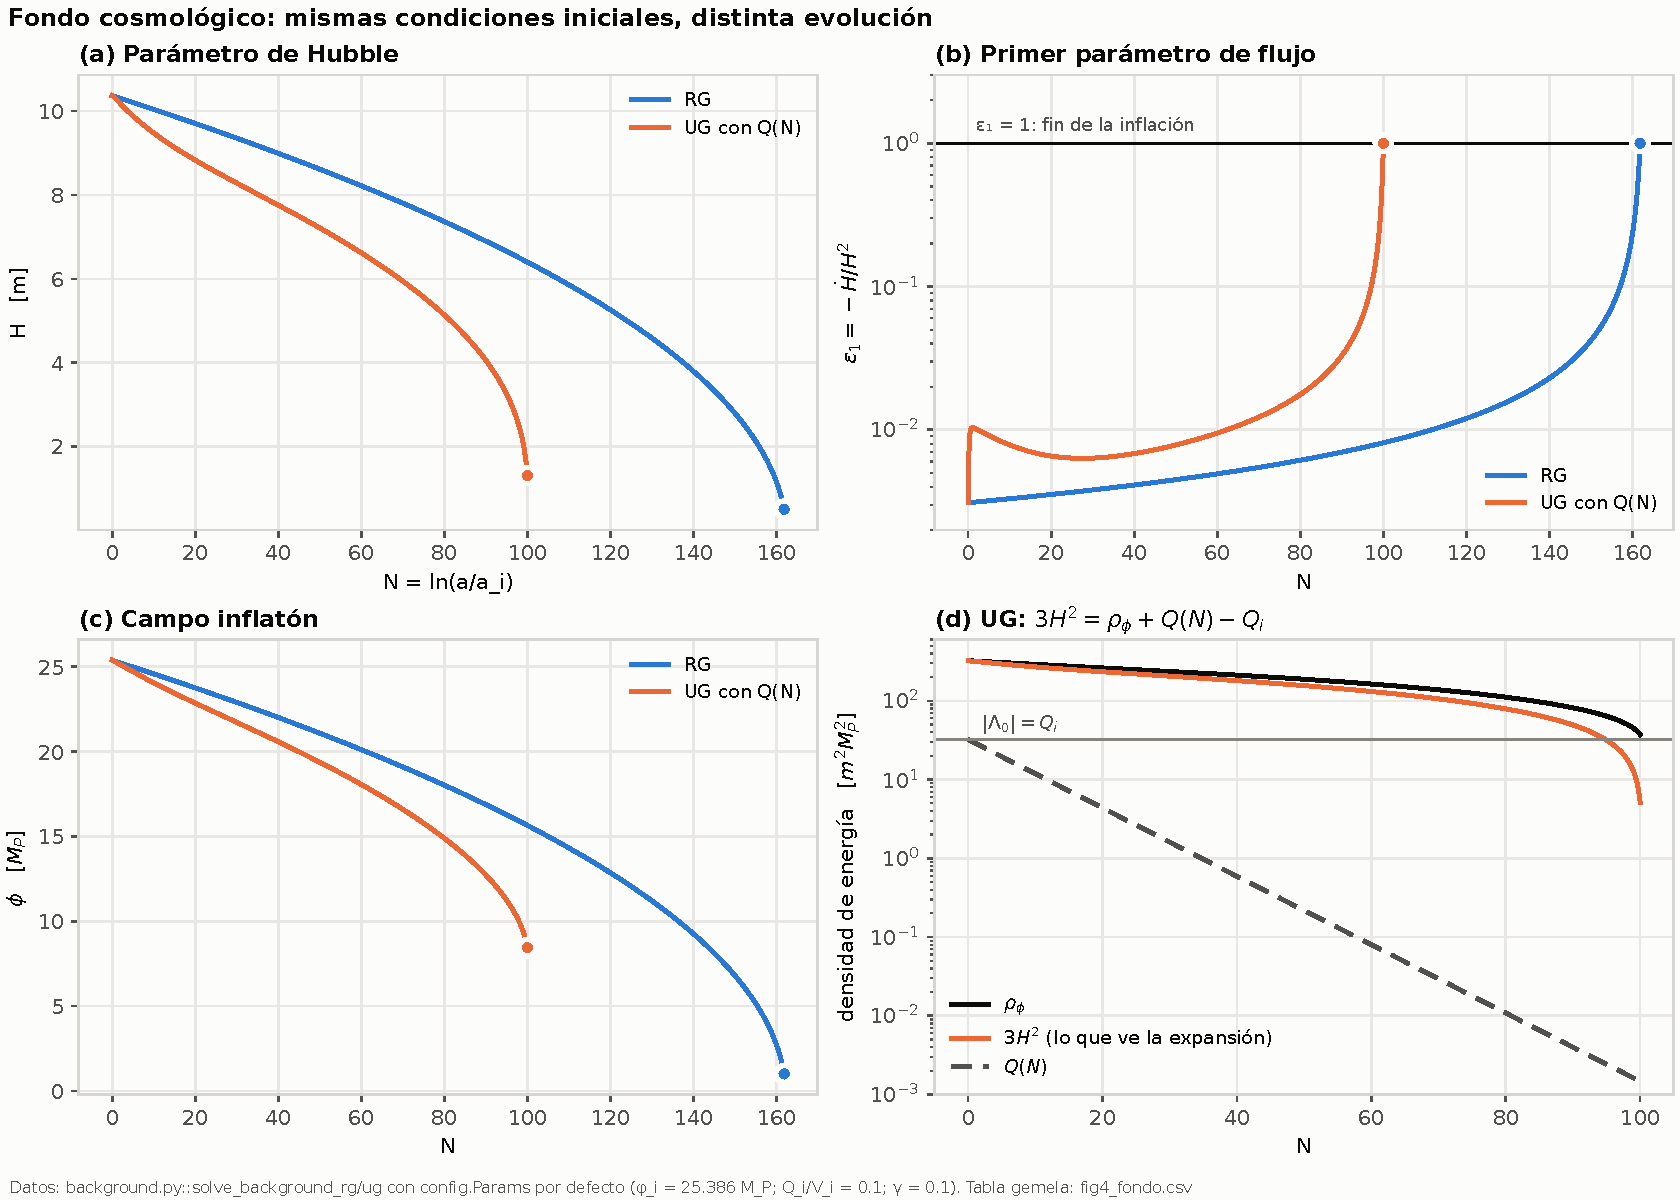
\includegraphics[width=\textwidth]{fig4_fondo.pdf}
\caption{Fondo cosmológico en RG (azul) y UG con difusión (naranja), con las mismas condiciones iniciales. (a) $H(N)$; (b) $\epsilon_1(N)$; (c) $\phi(N)$; (d) presupuesto de energía en UG: $3H^2=\rho_\phi+Q(N)-Q_i$. Generada por \texttt{make\_report\_figures.py}.}
\label{fig:fondo}
\end{figure}

Hay dos hechos de esta figura que hay que entender, porque condicionan el resto.

El primero es el salto inicial de $\epsilon_1$ de UG, que en el primer e-fold pasa de $0.0031$ a $0.0104$ (máximo en $N\simeq1.04$) y luego baja a un mínimo de $\sim0.006$. Se debe a que la velocidad inicial $\dot\phi_i$ es la de slow-roll de RG, que no está en el atractor de UG: el término $-\dot Q/\dot\phi$ de \eqref{eq:KGQ} es un empuje adicional que, en slow-roll, es del orden de $\gamma\,(Q/V)\,V^2/V'^2\times V'=\gamma\,(Q/V)\,(\phi^2/4)\,V'\simeq1.6\,V'$ al inicio (estimación de orden de magnitud). El campo se acelera hasta un nuevo régimen cuasi-estacionario en un e-fold. Es una consecuencia de imponer las mismas condiciones iniciales en ambos modelos, y no un error.

El segundo hecho es más importante, y no era evidente antes de graficar: \emph{el final de la inflación en UG no ocurre porque el campo llegue al fondo del potencial}. En $N=100$ el campo de UG está en $\phi=8.44\,\MP$, con $\rho_\phi=37.35$ y $\epsilon_V=2/\phi^2\simeq0.03$ (este epsilon del potencial desnudo no implica slow-roll del fondo UG, que tiene $\epsilon_1=1$; un universo de RG con ese mismo valor del campo tendría por delante unos $\phi^2/4-1/2\simeq17$ e-folds de inflación), pero $3H^2=5.13$. La razón está en el panel (d): como $Q(N)$ decae exponencialmente hasta $Q(100)=1.5\times10^{-3}$, la ecuación de Friedmann \eqref{eq:H2UG} con $\Lambda_0=-Q_i$ queda $3H^2=\rho_\phi-Q_i+Q\simeq\rho_\phi-32.2$: la constante de integración negativa le resta a $H^2$ una energía constante comparable a $\rho_\phi$ cuando este ha bajado a $\sim37$. Con $H^2$ tan pequeño, $\epsilon_1=\dot\phi^2/2H^2$ llega a $1$. Con más precisión: si $K=\dot\phi^2/2$ y $U=V+Q+\Lambda_0$ (en $\MP=1$), es $3H^2=K+U$ y $\epsilon_1=3K/(K+U)$, de modo que el criterio $\epsilon_1=1$ implementado equivale a $U=2K$, \emph{no} a $U=0$: al final, $3H^2=5.13$ da $K=1.71$ y $U=3.42>0$. La constante negativa $\Lambda_0=-Q_i$ resta a $U$ y adelanta ese instante respecto de RG, pero el final de la inflación no coincide con el cero del potencial efectivo. Es decir: en este modelo, la supresión de $H$ y el final temprano de la inflación en UG los produce en buena medida la elección $\Lambda_0=-Q_i$, que a su vez se sigue de pedir el mismo $H_i$ en ambos modelos. Esto se discute en la sección~\ref{sec:decisiones-dep}.

\subsection{Un modo a través del horizonte}

La figura~\ref{fig:modo} muestra la evolución de un modo individual con $k=2.12\times10^{18}\,m$, que sale del horizonte en $N=40.000$ en RG y en $N=40.149$ en UG. Antes del cruce, el modo oscila con amplitud constante (para $\tilde v$) y con oscilaciones que se van estirando en $N$ al acercarse al cruce, porque su frecuencia respecto de $N$ es $k/(aH)$ (panel b); es la oscilación de Bunch--Davies en un fondo en expansión. En el cruce, el $P_T$ instantáneo del modo, $2k^3|h|^2/\pi^2$, deja de decrecer y se congela (panel a). Los valores finales son $5.888\times10^{-10}$ en RG y $4.368\times10^{-10}$ en UG, con cociente $0.742$.

\begin{figure}[t]
\centering
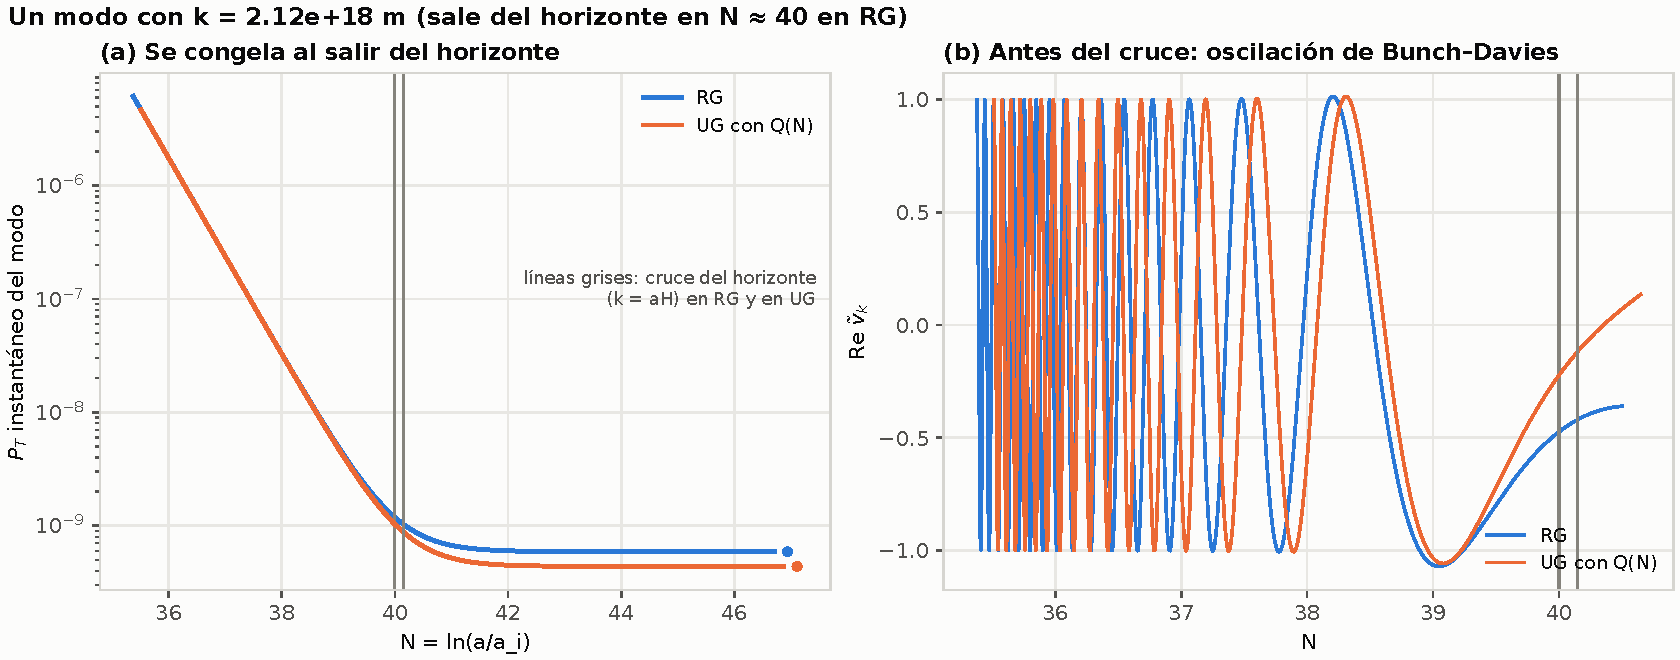
\includegraphics[width=\textwidth]{fig5_modo.pdf}
\caption{Un modo con $k=2.12\times10^{18}\,m$ en RG (azul) y UG (naranja). (a) $P_T$ instantáneo del modo; se congela al cruzar el horizonte (líneas grises). (b) Parte real de $\tilde v_k$ antes del cruce. Generada por \texttt{make\_report\_figures.py}.}
\label{fig:modo}
\end{figure}

Este cociente puede anticiparse casi sin integrar. En $N=40$ los parámetros de Hubble son $H_{\rm RG}=8.994$ y $H_{\rm UG}=7.760$, de modo que $(H_{\rm UG}/H_{\rm RG})^2=0.744$, que reproduce el valor numérico $0.742$ con la diferencia que cabe esperar de las correcciones de slow-roll y del pequeño corrimiento del instante de cruce. Es exactamente lo que dice la sección~\ref{sec:espectro}: el espectro se fija en el cruce del horizonte y depende de $H$ en ese instante.

\subsection{El espectro $P_T(k)$}

La figura~\ref{fig:PTk} es el resultado principal del cálculo: el espectro tensorial en RG y UG a igual $k$ comóvil, para $40$ modos entre $k=1.05\times10^4\,m$ y $k=3.48\times10^{39}\,m$ (un rango de $81.8$ en $\ln k$, limitado por la duración de la inflación de UG), con el cociente debajo.

\begin{figure}[t]
\centering
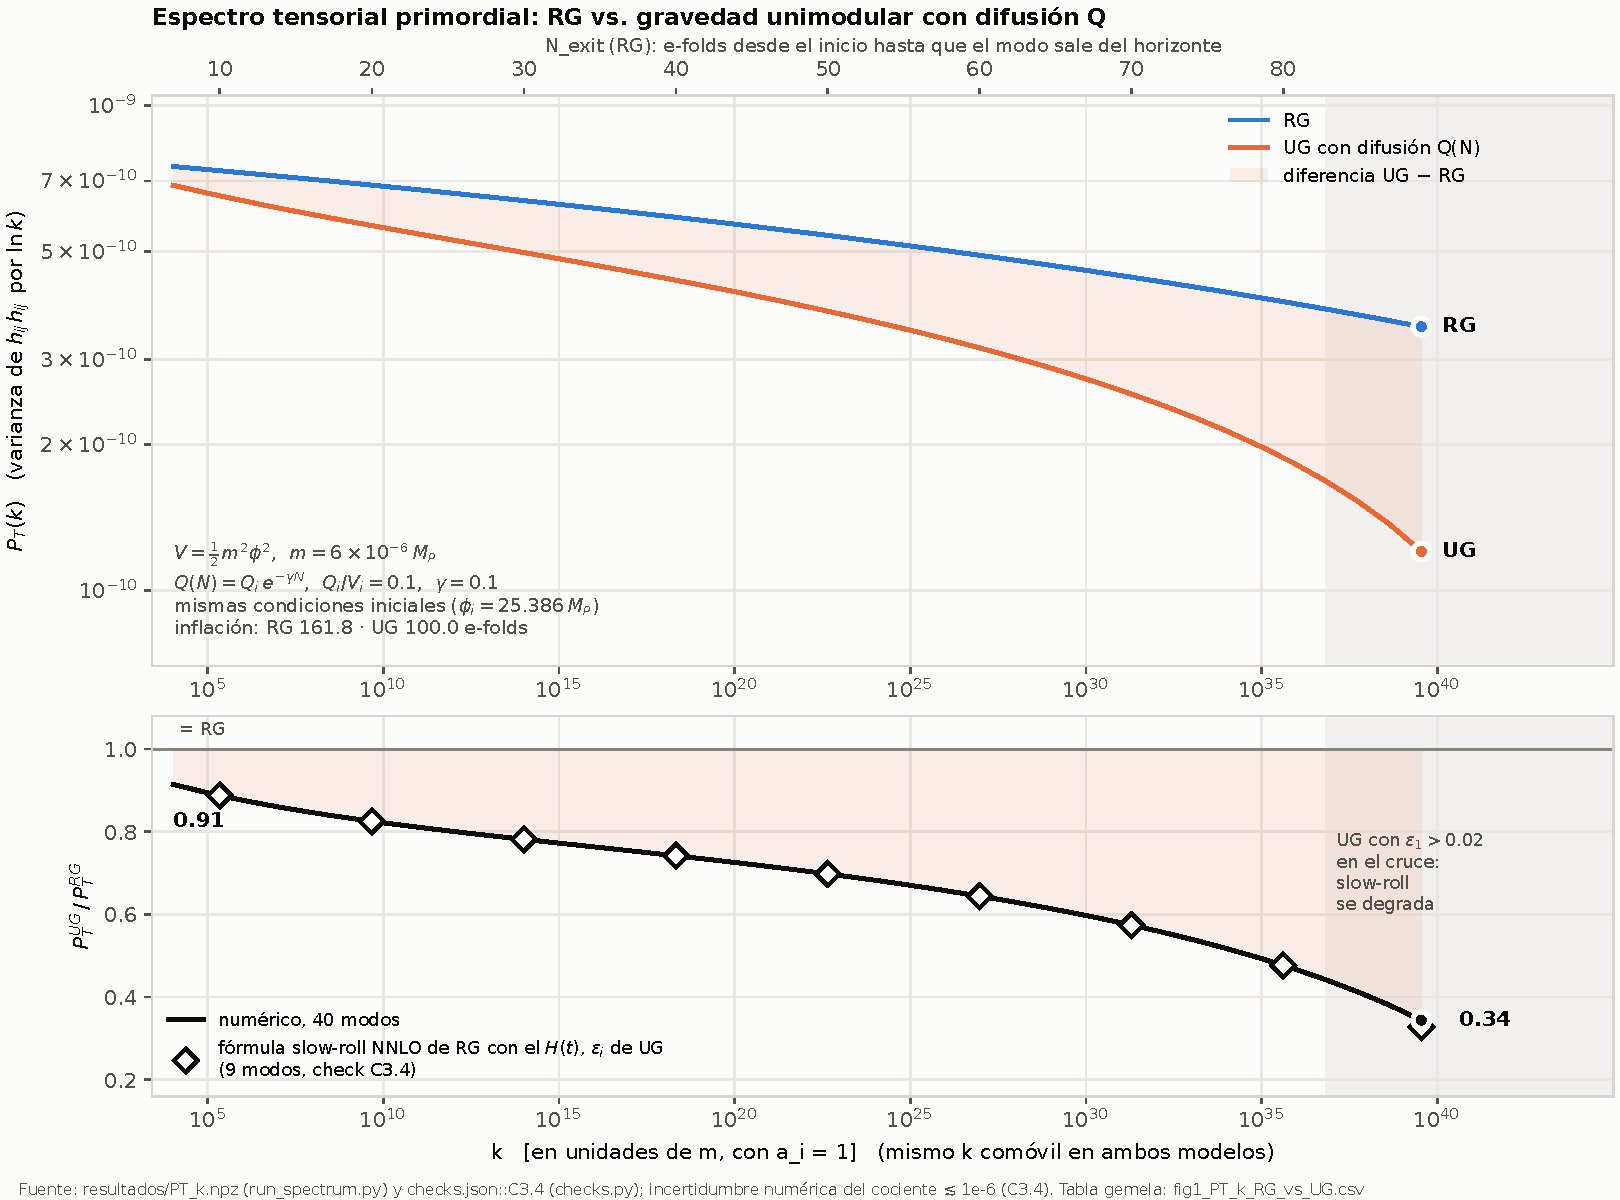
\includegraphics[width=\textwidth]{fig1_PT_k_RG_vs_UG.pdf}
\caption{Espectro tensorial primordial en RG y UG con difusión $Q(N)$. Arriba, $P_T(k)$ con la diferencia sombreada; abajo, el cociente UG/RG. Los marcadores huecos son la fórmula slow-roll de RG evaluada con el fondo de UG (control C3.4). La banda gris marca los modos donde $\epsilon_1^{\rm UG}>0.02$ en el cruce. El eje superior reetiqueta los mismos $k$ en e-folds. Generada por \texttt{make\_figures.py} a partir de los resultados guardados.}
\label{fig:PTk}
\end{figure}

En RG, $P_T$ decrece suavemente de $7.49\times10^{-10}$ a $3.50\times10^{-10}$ a lo largo del rango (una pendiente ligeramente roja, $n_T\simeq-2\epsilon_1$). En UG, para los mismos modos, decrece de $6.85\times10^{-10}$ a $1.21\times10^{-10}$. El cociente UG/RG va de $0.914$ en el primer modo a $0.344$ en el último, y en los nueve modos que se usan en los controles vale $0.888$, $0.825$, $0.782$, $0.742$, $0.698$, $0.644$, $0.574$, $0.477$ y $0.327$. Para estos parámetros, entonces, UG suprime $P_T$ frente a RG a igual $k$ en una cantidad que va del 8.6\% al 65.6\% según el modo. La banda gris marca la zona en que $\epsilon_1$ de UG en el cruce supera $0.02$, es decir, los modos que salen cuando la inflación de UG está terminando y la aproximación de slow-roll deja de ser buena: la magnitud del cociente ahí refleja en buena parte cuánto cae $H$ hacia el final, como se explicó en la sección~\ref{sec:fondores}.

Un punto a no perder de vista: los espectros se comparan a igual $k$ comóvil, con el mismo $a_i$ y las mismas condiciones iniciales, y como las dos inflaciones tienen duraciones distintas ($161.8$ y $100$ e-folds), la correspondencia entre un $k$ dado y ``$N$ e-folds antes del final de la inflación'' \emph{no} es la misma en los dos modelos. Por eso las figuras no deben leerse como una comparación a igual escala observacional, que requeriría modelar el recalentamiento y fijar un $k_*$ observable en cada modelo. \emph{La sección~\ref{sec:potenciales} muestra que esto no es un detalle: a igual número de e-folds antes del final de cada inflación el signo de la diferencia se invierte en el cuadrático} ($P_T^{\rm UG}/P_T^{\rm RG}=1.5$ en lugar de $0.3$--$0.9$). El resultado de esta subsección, ``UG suprime $P_T$'', vale solo a igual $k$ comóvil.

\subsection{Controles}

Los resultados anteriores se someten a diez controles reproducibles (nueve de resultado y uno de control de mutaciones), cada uno con tolerancia fijada \emph{antes} de correrlo y que no se modificó al ver los resultados; el código es \texttt{checks.py} y la evidencia legible por máquina es \texttt{checks.json}. Se los agrupa según lo que pretenden mostrar.

\subsubsection{El límite estándar de RG}

El primer control usa un fondo artificial de de Sitter exacto ($H$ constante, $\epsilon_1=0$), donde el modo de Bunch--Davies es analítico y $P_T=\frac{2H^2}{\pi^2\MP^2}(1+(k/aH)^2)$. El código reproduce esa expresión con un error relativo de $8.7\times10^{-7}$ para $k=10^3$, $10^5$ y $10^8$ (constante en $k$, como debe ser por la invariancia de escala). La solución a tiempo finito se obtiene de \cite[ecs.~196 y 198]{baumann22}, con la normalización tensorial usada aquí. Es una prueba a la vez del integrador, de la condición de Bunch--Davies, de la normalización de $P_T$ (incluido el factor de la sección~\ref{sec:normalizacion}) y de la forma en $N$ de la ecuación de modos. El error coincide en magnitud con el que produce el arranque en $k/aH=100$ en el barrido de convergencia.

El segundo compara, en RG con $V=\tfrac12m^2\phi^2$, el $P_T$ numérico con el desarrollo de slow-roll de Martin, Ringeval y Vennin \cite{martin14} a orden cero, uno y dos en los parámetros de flujo. La tabla~\ref{tab:sr} muestra el residuo relativo de $P_T/(2H^2/\pi^2\,a_0)-1$ en cuatro modos. A orden cero, la desviación es $-2(C+1)\epsilon_1$ (que es lo que predice \eqref{eq:PTNLO}); cada orden reduce el residuo, y a segundo orden queda por debajo de $6\times10^{-7}$ para $N_{\rm exit}=20$ a $100$, es decir, del orden del error de la condición inicial. En $N_{\rm exit}=140$, donde $\epsilon_1=0.023$, el residuo es $-4\times10^{-5}$ (unas $3\epsilon_1^3$, el tamaño esperado del término de orden siguiente).

\begin{table}[t]
\centering\small
\renewcommand{\arraystretch}{1.2}
\begin{tabular}{@{}rcccc@{}}
\toprule
$N_{\rm exit}$ & $\epsilon_1$ & LO & NLO & NNLO\\
\midrule
20 & 0.0035 & $-1.92\times10^{-3}$ & $-1.15\times10^{-5}$ & $+4.9\times10^{-7}$\\
60 & 0.0049 & $-2.69\times10^{-3}$ & $-2.28\times10^{-5}$ & $+5.0\times10^{-7}$\\
100 & 0.0081 & $-4.45\times10^{-3}$ & $-6.38\times10^{-5}$ & $-2.9\times10^{-7}$\\
140 & 0.0230 & $-1.30\times10^{-2}$ & $-5.51\times10^{-4}$ & $-4.1\times10^{-5}$\\
\bottomrule
\end{tabular}
\caption{Residuo relativo de $P_T$ numérico (RG, $\phi^2$) frente al desarrollo de slow-roll a orden cero (LO), uno (NLO) y dos (NNLO), evaluado en el cruce del horizonte.}
\label{tab:sr}
\end{table}

El tercero es la comparación con las predicciones conocidas de $V\propto\phi^2$. Para $N_*=60$ e-folds antes del final, el cálculo da $\epsilon_1=0.00836$, una relación $r=P_T/P_\mathcal{R}^{\rm LO}=0.1332$ (usando $P_\mathcal{R}=H^2/8\pi^2\epsilon_1$ de \eqref{eq:PRr} con el $H$ y el $\epsilon_1$ del código), que es 99.5\% de $16\epsilon_1=0.1338$; y para $N_*=50$, $r=0.1597$. Están dentro del rango de ``aproximadamente $0.15$'' que Planck da para el potencial cuadrático \cite{planck20}. La pendiente tensorial, medida como diferencia finita en $\ln k$ entre modos, coincide con la de la fórmula de \cite{martin14} a $2\times10^{-6}$: $n_T=-0.016947$ frente a $-0.016945$ (y $-2\epsilon_1=-0.016727$ a orden más bajo). Finalmente, la amplitud escalar $A_s=P_\mathcal{R}^{\rm LO}m_{\rm phys}^2$ a $N_*=60$ es $2.167\times10^{-9}$, frente al valor de Planck $2.099\times10^{-9}$ ($\ln10^{10}A_s=3.044$): una diferencia de $+3.2$\%, que valida el valor $m=6\times10^{-6}\MP$ elegido. Este último control usa la fórmula estándar del espectro escalar de RG, no un cálculo propio.

\subsubsection{Convergencia numérica}

Se varía un parámetro numérico por vez y se compara con un valor de referencia más fino, en cuatro modos y en RG y UG (figura~\ref{fig:conv}). Con los valores por defecto el resultado es estable a $\sim10^{-6}$: las tolerancias de los integradores contribuyen menos de $10^{-9}$, la resolución de los splines del fondo no se distingue de $4\times10^{-13}$ a partir de $2\,001$ puntos, y las dos fuentes dominantes son la condición inicial (el arranque en $k/aH=100$ da $9.0\times10^{-7}$, y cae como $(aH/k)^3$: $3.6\times10^{-5}$ para $30$, $3.8\times10^{-8}$ para $300$) y el punto de medida ($10^{-6}$, el $(k/aH)^2$ esperado). Los cinco valores por defecto están dentro de su tolerancia a priori.

\begin{figure}[t]
\centering
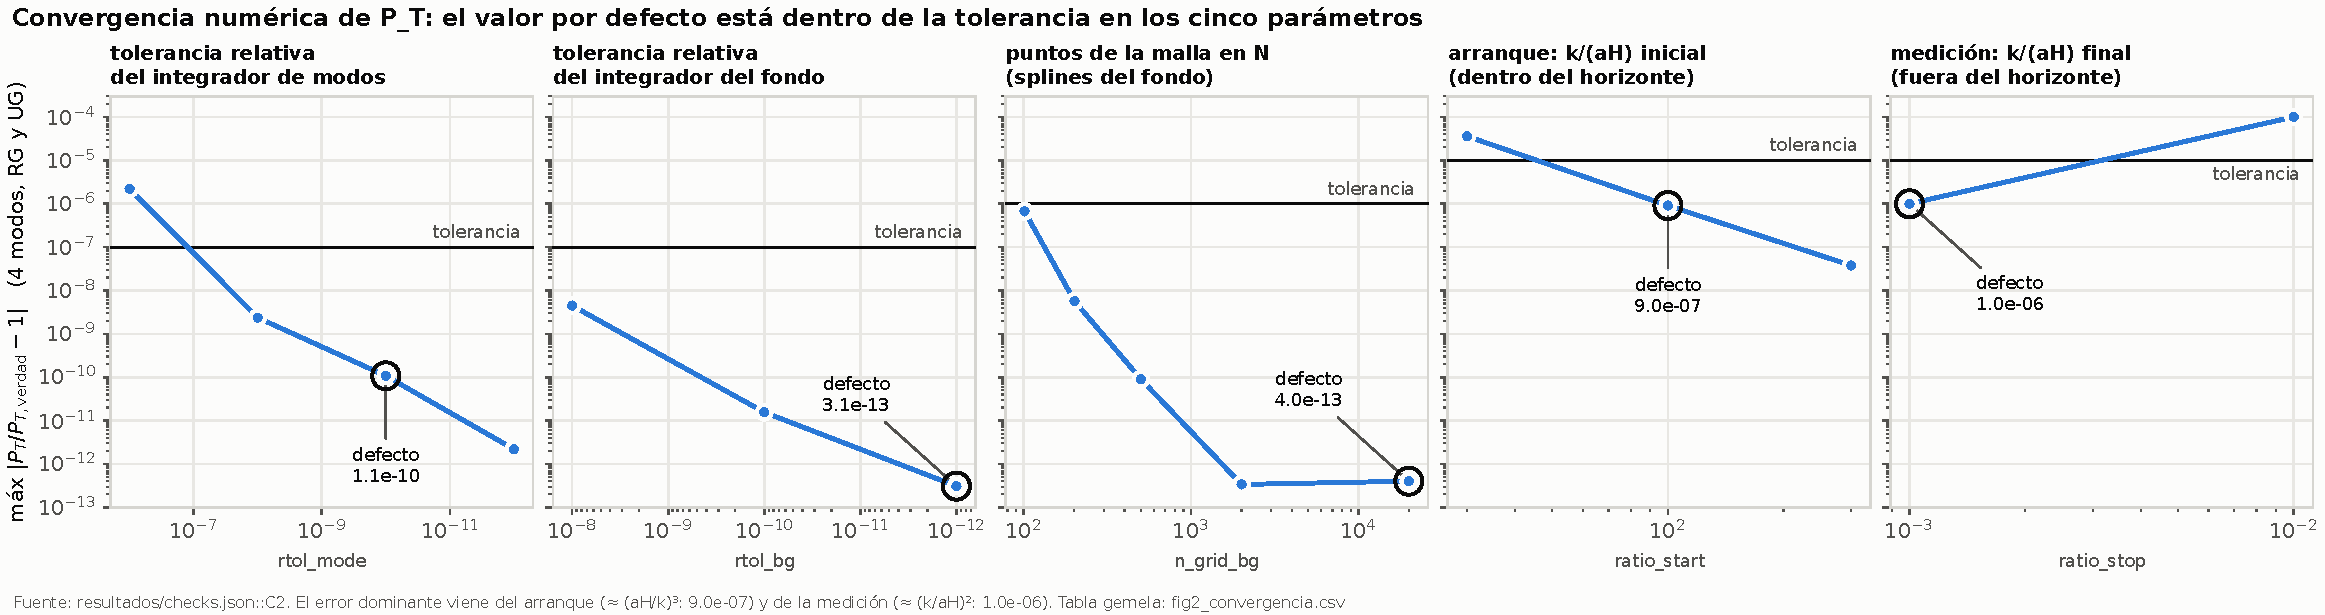
\includegraphics[width=\textwidth]{fig2_convergencia.pdf}
\caption{Convergencia numérica de $P_T$: error máximo frente a un valor de referencia más fino, variando un parámetro por vez (cuatro modos, RG y UG). La línea es la tolerancia fijada a priori y el círculo marca el valor por defecto.}
\label{fig:conv}
\end{figure}

\subsubsection{La diferencia entre UG y RG}

\begin{figure}[t]
\centering
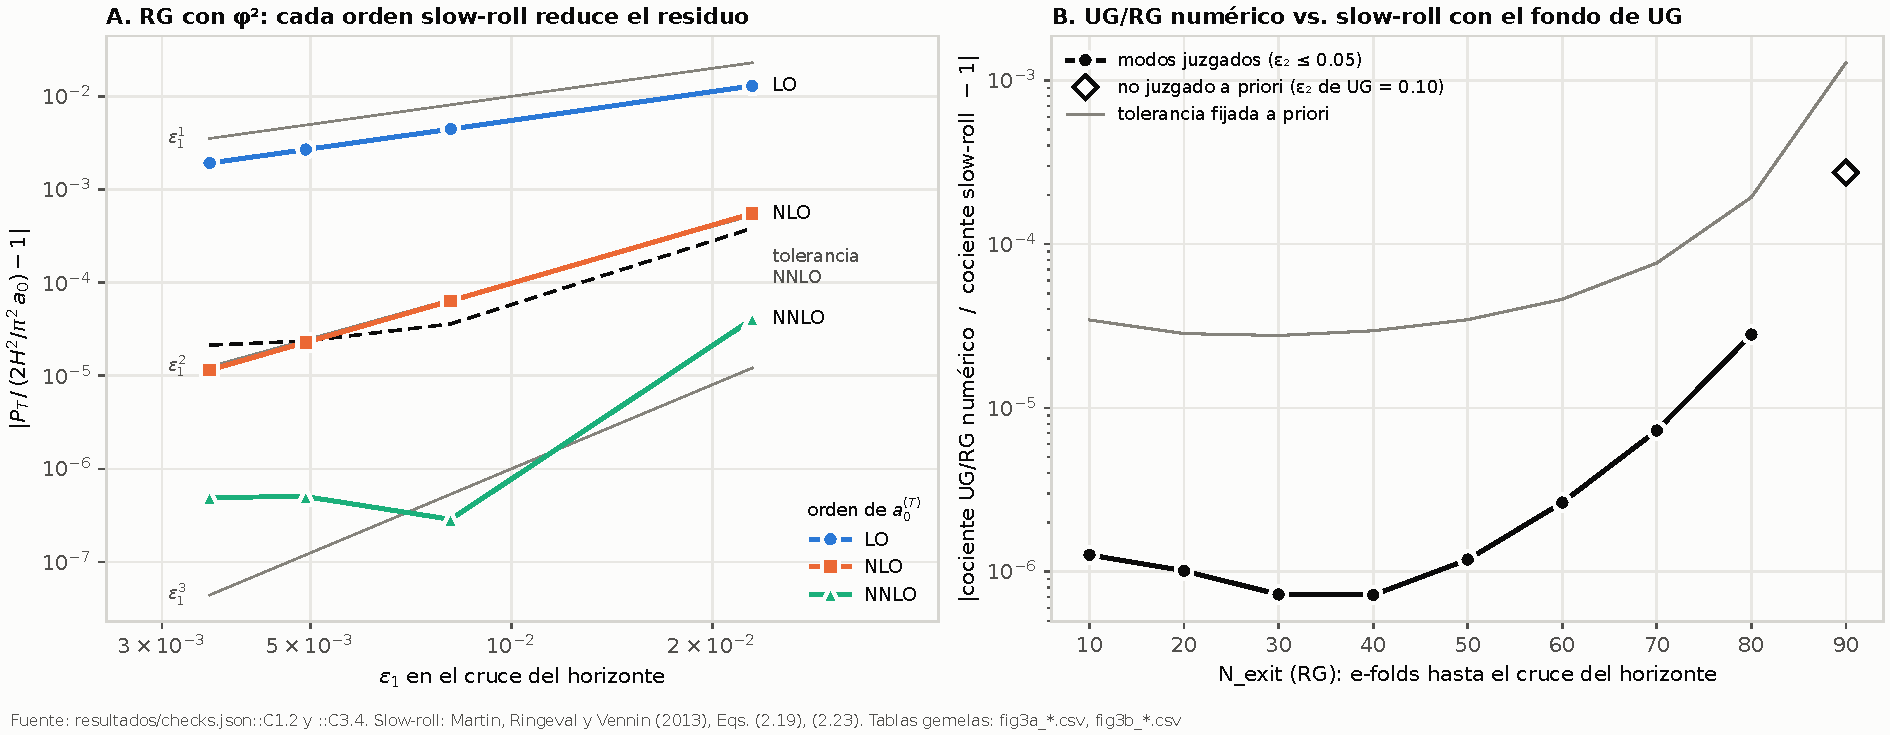
\includegraphics[width=\textwidth]{fig3_limite_estandar.pdf}
\caption{(A) RG con $\phi^2$: residuo de $P_T$ frente al desarrollo de slow-roll a tres órdenes. (B) El cociente UG/RG numérico frente al de la fórmula de slow-roll de RG evaluada con el fondo de UG.}
\label{fig:limite}
\end{figure}

Para que la diferencia de la figura~\ref{fig:PTk} sea un resultado, tiene que descartarse que sea un error numérico, y hay que entender de dónde viene. Se hicieron cinco comprobaciones (a las que se suma la de sensibilidad de la sección siguiente).

Primero, el ruido: recalculando el cociente con distintas tolerancias de los integradores, con otro punto de arranque y con otro punto de medida, cambia como máximo $8.5\times10^{-7}$ (dominado por el arranque), frente a una señal mínima de $0.112$: un cociente entre la diferencia de modelos y el error numérico estimado de $1.3\times10^{5}$ (es un cociente de tamaños numéricos, no una significancia estadística ni una detectabilidad experimental). Segundo, se compara el cociente numérico con el que da la fórmula de slow-roll de RG \eqref{eq:cociente} evaluada con el $H$, $\epsilon_1$ y $\epsilon_2$ \emph{propios de UG} en su cruce del horizonte (figura~\ref{fig:limite}B): coinciden a $\lesssim3\times10^{-5}$ en los ocho modos donde se aplica el criterio fijado a priori ($\epsilon_1$ y $|\epsilon_2|$ de ambos modelos menores que $0.05$), la mayoría a $\sim10^{-6}$, y en el noveno (con $\epsilon_2^{\rm UG}=0.10$, fuera del criterio) la diferencia es $2.7\times10^{-4}$. Tercero, un control de consistencia entre los dos códigos: con $\gamma=0$ ($Q$ constante y $\Lambda_0=-Q_i$), UG debe ser RG exacta (sección~\ref{sec:difusionQ}), y así ocurre a $4.3\times10^{-13}$ en $P_T$ y $8.5\times10^{-14}$ en la duración: prueba el camino de UG del código (\texttt{quantities\_ug}, la ecuación \eqref{eq:KGQ} con $\dot Q$ y \eqref{eq:Lambda0}) contra el de RG, que son funciones distintas. Cuarto, la ecuación \eqref{eq:HdotUG}, que no se usó para construir el fondo, se verifica sobre la solución integrada: $|\!-\!\dd\ln H/\dd N-\phi_N^2/2|$ es a lo sumo $7.9\times10^{-12}$ en RG y $3.0\times10^{-7}$ en UG (en $N=0$, donde $\epsilon_1$ de UG salta). Quinto, un integrador independiente de la ecuación \eqref{eq:modoX}, escrito en tiempo cósmico, para $h$ y sin usar $N$, $v$, $\epsilon_1$ ni splines, coincide con el de \texttt{modes.py} a $4.4\times10^{-10}$ en RG y UG; valida los pasos que llevan de \eqref{eq:modoX} a \eqref{eq:modoN}.

\subsubsection{Que los controles puedan detectar errores}

Un control que nunca falla no prueba nada, y por eso se agregan dos comprobaciones de sensibilidad. Un control negativo: si se calcula el modo de UG con un $\Lb$ equivocado (omitiendo $Q$, de modo que $X\neq0$ y aparece una masa efectiva $-2X$), $P_T$ cambia en un 60\% para $N_{\rm exit}=12$, 7.6\% para $40$, 0.7\% para $70$ y 0.3\% para $85$ (la sensibilidad decrece porque $Q\propto\ee^{-\gamma N}$). Con el $X$ que se calcula frente a forzar $X=0$, el cambio es menor que $5\times10^{-14}$: el término de masa calculado es despreciable. Y un control de mutaciones: se rompe el código a propósito de tres maneras (duplicar la normalización de $P_T$, cambiar el signo de $\epsilon_1$ en la ecuación de modos, y desplazar $\Lambda_0$ en 0.01\% de $Q_i$) y se verifica que los cuatro controles correspondientes fallan (el cambio de signo de $\epsilon_1$ debe ser detectado por dos de ellos).

\subsection{Balance de los controles}

Los diez controles pasan, y también la batería completa de pruebas automáticas (17 en el momento de esta sección, contando la sincronía del notebook con el código y las pruebas de las figuras; las secciones~\ref{sec:potenciales} y~\ref{sec:acoplamiento} agregan ocho de Starobinsky y cuatro simbólicas). Vale la pena decir qué muestran y qué no. Muestran que el código reproduce el límite estándar de RG con la precisión que se le pide, que su resultado es estable frente a los parámetros numéricos, y que la diferencia entre UG y RG es real y se explica por el fondo. \emph{No} muestran que la derivación analítica sea correcta: el control de atribución valida la numérica, y la ecuación de modos de UG que integra el código es, por construcción, la de la derivación con el término de masa que se demostró que se anula; el único control que podría contradecirla es el de sensibilidad (que dice que, si no se anulara, el código lo vería), pero éste no la comprueba de manera independiente. Tampoco hay una referencia externa contra la cual comparar $P_T$ de UG con difusión, porque no se conoce una en la literatura leída; UG se apoya en consistencia interna y con RG. Estos límites se retoman en la sección~\ref{sec:discusion}.

\section{Un segundo potencial y la comparación a igual $N_*$}
\label{sec:potenciales}

Los resultados de la sección~\ref{sec:resultados} se obtuvieron con un solo potencial y comparando a igual $k$ comóvil. Esta sección corrige ambas limitaciones. Agrega un segundo potencial, el de Starobinsky, y cambia el criterio de comparación por uno que no depende de que los dos modelos duren lo mismo. El resultado es que \emph{una de las conclusiones de la sección~\ref{sec:resultados} no sobrevive} al cambio de criterio, y hay que leerla con la salvedad que se explica en la subsección~\ref{sec:igualN}.

\subsection{Por qué otro potencial}
\label{sec:porquestaro}

El potencial cuadrático se adoptó por ser el más simple, con un solo parámetro que solo escala la amplitud. Tiene dos inconvenientes conocidos. Predice $r\approx0.13$--$0.16$ para $N_*=60$--$50$, que está en tensión con las observaciones (sección~\ref{sec:GW-RG}, \cite{planck20,bicep21}); y el campo recorre $\phi_*\approx15\,\MP$ durante las últimas 60 e-folds. Además, el resultado de UG dependía de un rasgo propio de este potencial: la energía $\rho_\phi$ cae hasta ser comparable con $Q_i$ al final de la inflación, y por eso la constante $\Lambda_0=-Q_i$ termina la inflación de UG (sección~\ref{sec:fondores}).

El potencial de Starobinsky,
\begin{equation}
V(\phi)=\tfrac34\,M^2\MP^2\big(1-\ee^{-\sqrt{2/3}\,\phi/\MP}\big)^2,
\label{eq:Vstaro}
\end{equation}
es un plateau: para $\phi\gg\MP$ es casi constante y el slow-roll vale con $\epsilon_1\approx3/(4N^2)$, de modo que $r\approx12/N^2\approx3\times10^{-3}$ y $n_s\approx1-2/N$ para $N=60$ \etq{E}. Aquí se adopta fenomenológicamente la forma \eqref{eq:Vstaro} \etq{S}. Las referencias históricas \cite{starobinsky80,defelice10} se verificaron solo en metadatos; no se usa su contenido como verificación textual de una transformación conforme ni se deriva un origen $R^2$ en UG. El control numérico contrasta las estimaciones estándar $r\approx12/N^2$ y $n_s\approx1-2/N$.

La escala $M$ es una calibración, no una predicción: se fijó en $M=1.14\times10^{-5}\,\MP$ para que RG reproduzca la amplitud escalar de Planck, $A_s=2.10\times10^{-9}$ \cite{planck20}, a $N_*=60$ con la fórmula de orden cero $P_\mathcal{R}=H^2/(8\pi^2\MP^2\epsilon_1)$. Un valor de memoria que tenía antes ($1.3\times10^{-5}$) correspondía a $N_*\approx52$ y se descartó antes de correr los controles. Como en el caso cuadrático, $M$ solo escala $P_T$ (por homogeneidad, el código integra con $M=1$).

El resto de las decisiones no cambia: mismos $\phi_i$, $\dot\phi_i$ y $H_i$ en RG y UG; $\Lambda_0=-Q_i$; $Q(N)=Q_i\ee^{-\gamma N}$ con $Q_i/V_i=0.1$ y $\gamma=0.1$; y $\phi_i$ ajustado para que UG dure $N_f=100$ e-folds, lo que da $\phi_i=7.660\,\MP$.

\subsection{El fondo de UG con Starobinsky}
\label{sec:fondostaro}

La figura~\ref{fig:fondostaro} muestra el fondo. Hay tres diferencias con el caso cuadrático que importan para lo que sigue.

\begin{figure}[t]
\centering
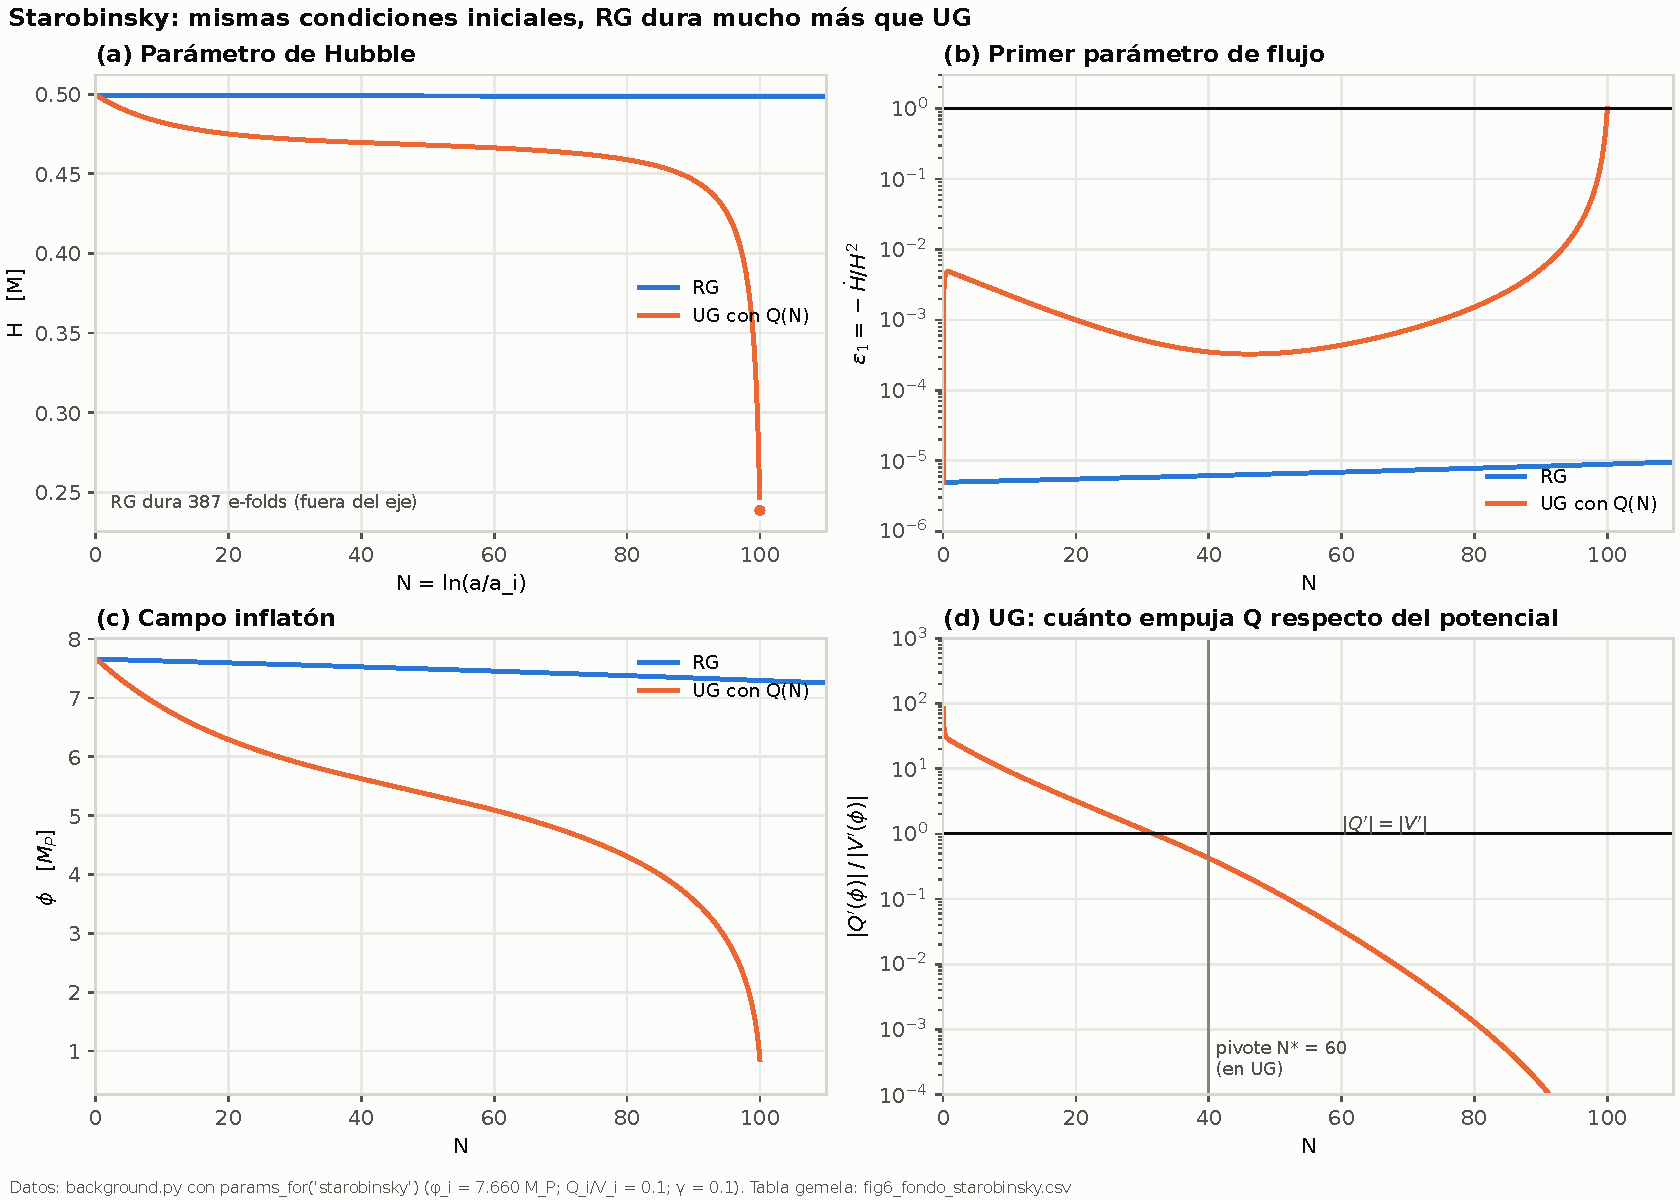
\includegraphics[width=\textwidth]{fig6_fondo_starobinsky.pdf}
\caption{Fondo de RG y UG con el potencial de Starobinsky, con las mismas condiciones iniciales. (a) $H(N)$; (b) $\epsilon_1(N)$; (c) $\phi(N)$; (d) razón $|Q'(\phi)|/|V'(\phi)|$ entre el empuje de $Q$ y el del potencial en UG, con $Q'=(\dd Q/\dd N)/(\dd\phi/\dd N)$. Generada por \texttt{make\_figures\_potenciales.py}.}
\label{fig:fondostaro}
\end{figure}

\emph{Duración.} Con el mismo $\phi_i$, RG dura $386.7$ e-folds y UG $100$ (en el cuadrático eran $161.8$ y $100$). En RG las primeras $\sim300$ e-folds transcurren en el plateau, con $\epsilon_1\sim10^{-6}$; ahí $H$ es casi constante (panel a).

\emph{Un transitorio inicial dominado por $Q$.} La velocidad inicial $\dot\phi_i=-V'/\sqrt{3V}$ es la de slow-roll de $V$ sola y queda unas treinta veces por debajo del atractor de UG. En UG el término $-\dot Q/\dot\phi$ de \eqref{eq:KGQ} lo compensa en una fracción de e-fold: $\epsilon_1$ salta de $5\times10^{-6}$ a $1.3\times10^{-3}$ en $\Delta N=0.05$ (panel b). El cociente $|Q'|/|V'|$ (panel d) es del orden de $10^2$ al inicio, $9$ en $N=10$, $1.2$ en $N=30$, $0.4$ en $N=40$ y $0.03$ en $N=60$: durante las primeras $\sim30$ e-folds el inflatón de UG está empujado más por $Q$ que por el potencial, y a partir de $N\approx50$ la dinámica es la de Starobinsky. Es una consecuencia de imponer las mismas condiciones iniciales y de la forma de $Q(N)$, y no una propiedad de UG.

\emph{El final de la inflación.} Al terminar ($\epsilon_1=1$) es $3H^2\approx0.20$ y $V\approx0.23$ (en unidades de $M^2\MP^2$): el presupuesto energético del ejemplo satisface $U=2K$ al evento $\epsilon_1=1$. Estos valores no aíslan la contribución causal de $\Lambda_0$; no se realizó una comparación controlada variando esa constante con las demás condiciones fijadas. Una extensión en la que $Q$ tienda a cero y el campo alcance el mínimo de $V$ dejaría una contribución efectiva negativa por $\Lambda_0=-Q_i$. Esa extrapolación requiere extender la prescripción $Q(N)$ y la solución después de la inflación; no se integró esa etapa ni se demuestra un futuro anti-de Sitter.

\subsection{Por qué comparar a igual $N_*$}
\label{sec:igualN}

La figura~\ref{fig:igualk} muestra la comparación a igual $k$ (la de la sección~\ref{sec:resultados}) para los dos potenciales. En el cuadrático UG suprime $P_T$ (de $0.914$ a $0.344$); en Starobinsky lo suprime menos (de $0.947$ a $0.796$).

\begin{figure}[t]
\centering
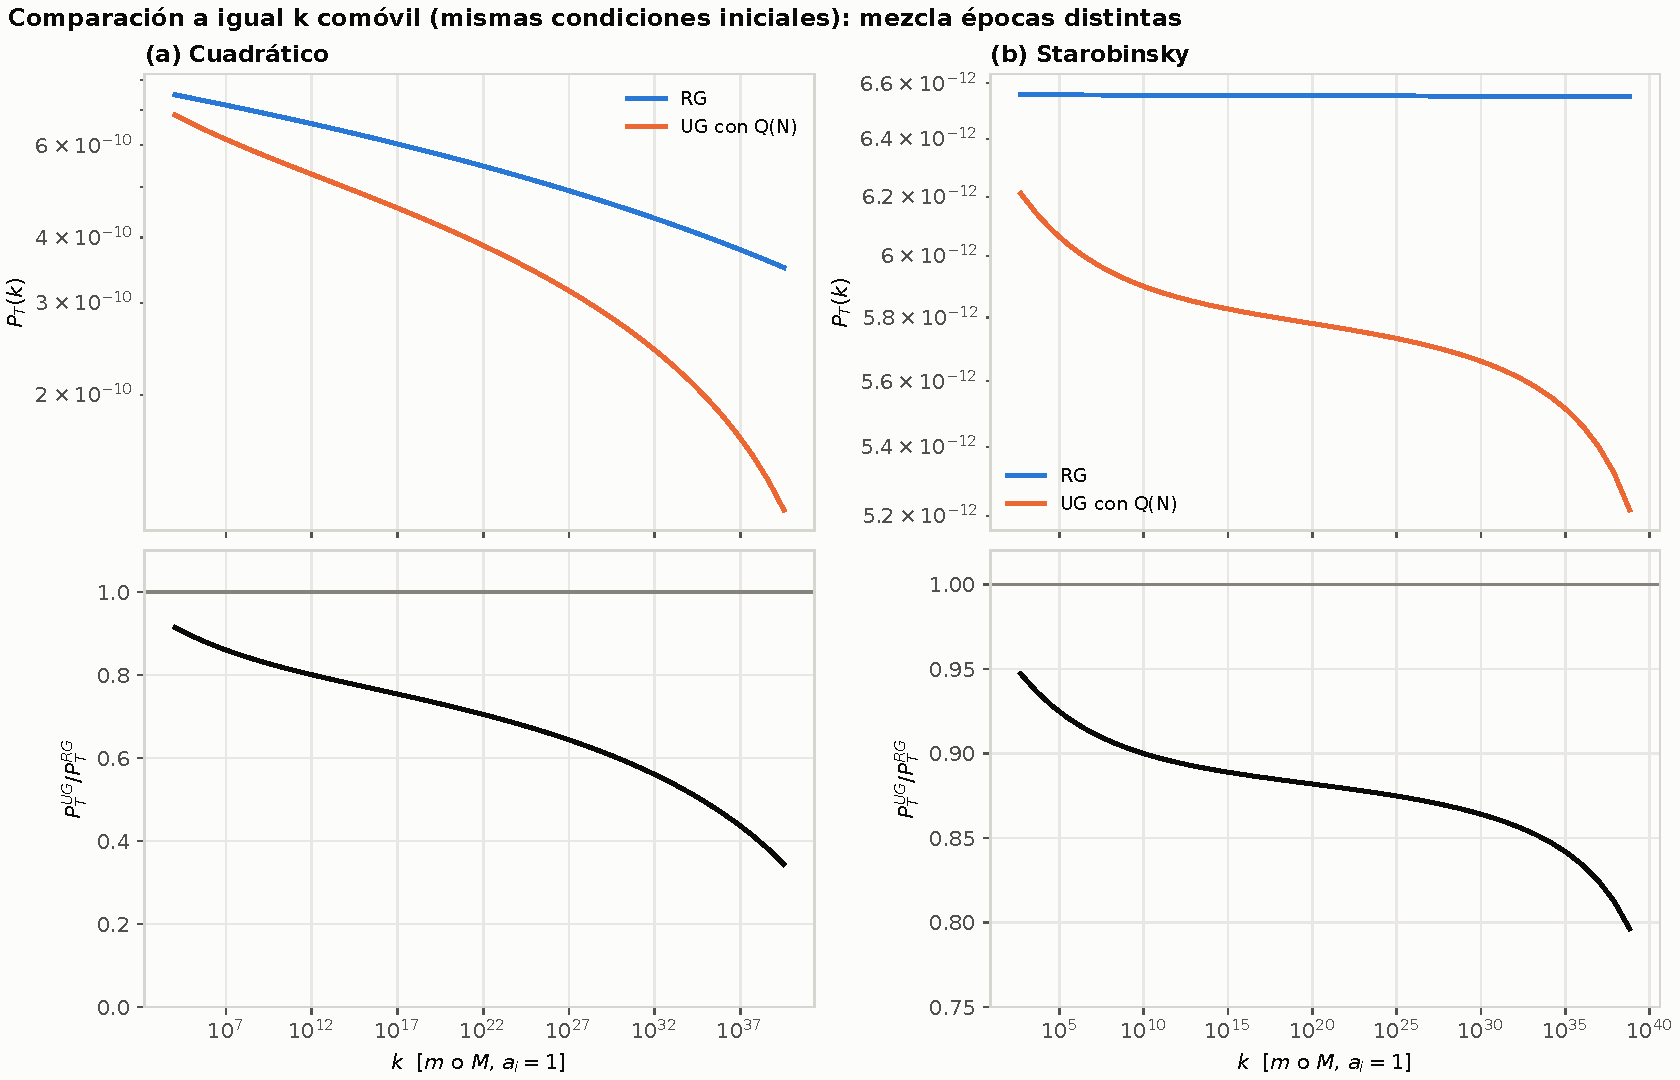
\includegraphics[width=\textwidth]{fig7_igual_k_potenciales.pdf}
\caption{Comparación a igual $k$ comóvil (mismo $a_i$ y mismas condiciones iniciales), cuadrático y Starobinsky. Arriba $P_T(k)$; abajo el cociente UG/RG. Datos de \texttt{run\_spectrum.py} (\texttt{resultados/PT\_k.csv} y \texttt{resultados/starobinsky/PT\_k.csv}); generada por \texttt{make\_figures\_potenciales.py}.}
\label{fig:igualk}
\end{figure}

Pero ese criterio compara épocas distintas. Con el mismo $a_i$ y la misma $k$, los cruces se obtienen resolviendo $k=aH$ por separado y, como $H$ difiere, no ocurren en el mismo $N$, mientras que la inflación termina en $N_{\rm end}=161.8$ (RG) y $100$ (UG) en el cuadrático, y en $386.7$ y $100$ en Starobinsky. En Starobinsky, por ejemplo, el instante $N=40$ está 347 e-folds antes del final de RG y 60 antes del final de UG; los modos que cruzan en ese instante tienen distinto $k$: no es la misma escala observacional. Lo que se compara con datos es $P_T$ y $n_T$ en el modo que salió del horizonte $N_*$ e-folds antes del final de \emph{la propia inflación} (la relación con la escala observable requeriría además modelar el recalentamiento, que no se hace). Por eso se agrega como resultado principal la comparación a igual $N_*$, con $N_*=50$ y $60$ en cada modelo, y se deja la de igual $k$ como secundaria. El script es \texttt{compare\_potentials.py}.

\subsection{Resultados a igual $N_*$}
\label{sec:resultadosN}

\begin{table}[t]
\centering\small
\renewcommand{\arraystretch}{1.2}
\begin{tabular}{@{}llrrrrrr@{}}
\toprule
Potencial & $N_*$ & $P_T^{\rm UG}/P_T^{\rm RG}$ & $n_T^{\rm RG}$ & $n_T^{\rm UG}$ & $r_{\rm std}^{\rm RG}$ & $r_{\rm std}^{\rm UG}$ & $n_{s,{\rm std}}^{\rm UG}$\\
\midrule
cuadrático  & 50 & 1.575 & $-2.04\times10^{-2}$ & $-1.59\times10^{-2}$ & 0.160 & 0.125 & 0.968\\
cuadrático  & 60 & 1.516 & $-1.70\times10^{-2}$ & $-1.38\times10^{-2}$ & 0.133 & 0.109 & 0.975\\
Starobinsky & 50 & 0.902 & $-5.5\times10^{-4}$ & $-6.7\times10^{-4}$ & $4.4\times10^{-3}$ & $5.4\times10^{-3}$ & 0.986\\
Starobinsky & 60 & 0.904 & $-3.9\times10^{-4}$ & $-7.0\times10^{-4}$ & $3.1\times10^{-3}$ & $5.6\times10^{-3}$ & 1.022\\
\bottomrule
\end{tabular}
\caption{Comparación a igual $N_*$ (e-folds antes del final de la inflación de cada modelo), con $m=6\times10^{-6}\MP$ y $M=1.14\times10^{-5}\MP$. $P_T$ y $n_T$ son resultados. $r_{\rm std}=P_T/P_\mathcal{R}^{\rm LO}$ y $n_{s,{\rm std}}=1-2\epsilon_1-\epsilon_2$ usan la fórmula escalar \emph{estándar de RG evaluada con el fondo de UG}: para UG son condicionales, porque el sector escalar con difusión no está derivado (sección~\ref{sec:abiertos}). Datos: \texttt{resultados/comparacion\_N\_star.csv}.}
\label{tab:igualN}
\end{table}

\begin{figure}[t]
\centering
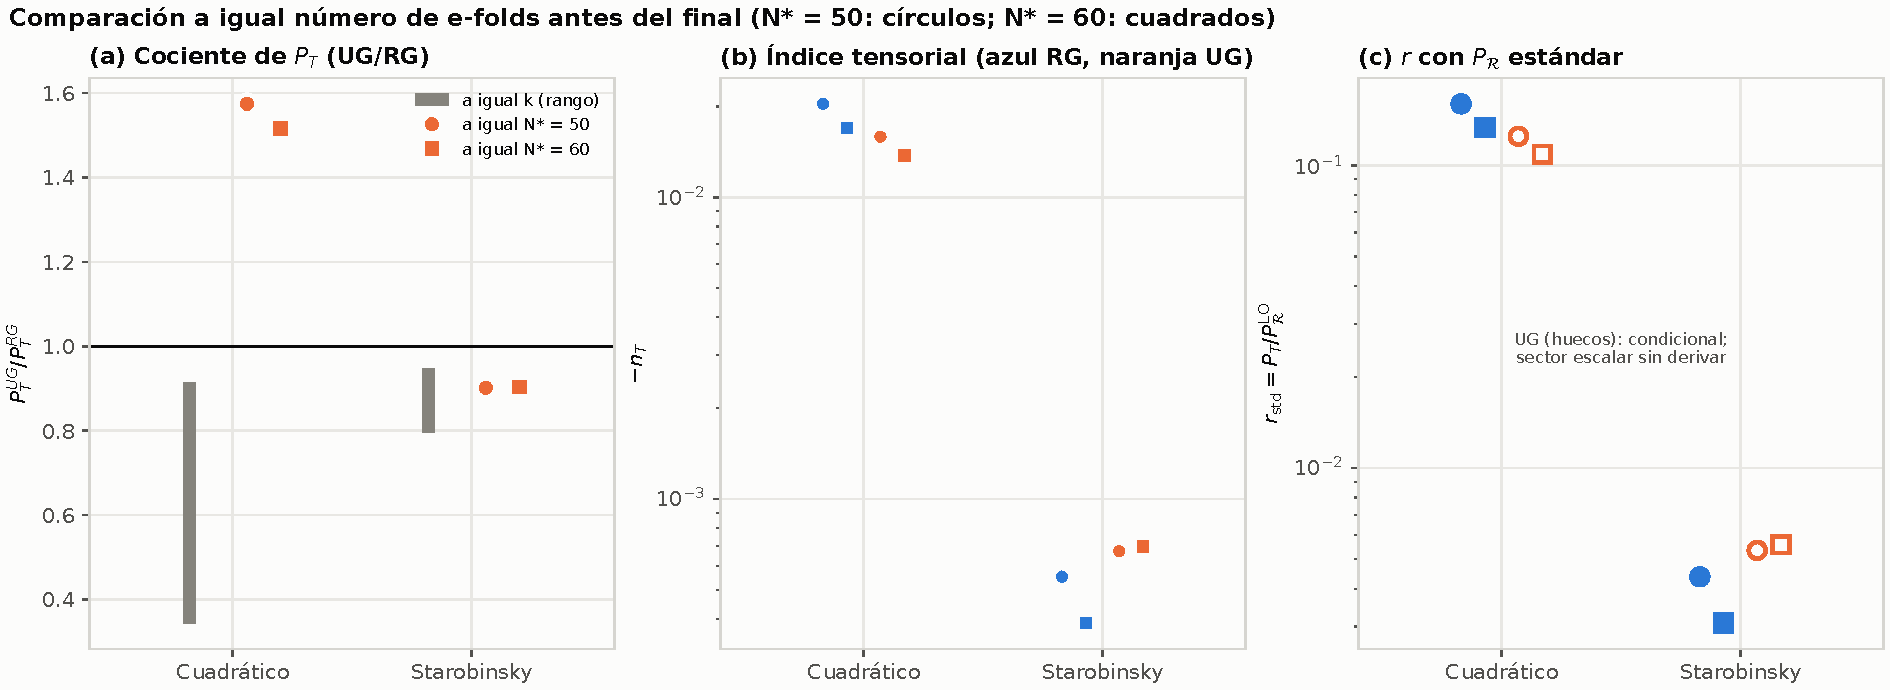
\includegraphics[width=\textwidth]{fig8_igual_Nstar.pdf}
\caption{Comparación a igual $N_*$ para los dos potenciales. (a) Cociente $P_T^{\rm UG}/P_T^{\rm RG}$ a igual $N_*$ (marcadores naranja) y su rango a igual $k$ (barra gris). (b) $-n_T$. (c) $r_{\rm std}$, con UG condicional (huecos). Generada por \texttt{make\_figures\_potenciales.py}.}
\label{fig:igualN}
\end{figure}

El resultado, resumido en la tabla~\ref{tab:igualN} y la figura~\ref{fig:igualN}, es doble.

\emph{En el cuadrático el signo de la diferencia depende del criterio.} A igual $k$ UG suprime $P_T$ (por un factor entre $0.914$ y $0.344$); a igual $N_*$ lo \emph{aumenta} (por $1.5$--$1.6$). Con la masa $m$ fija en ambos modelos, la razón es que la inflación de UG termina antes en el potencial (con $\phi\approx8.4\,\MP$, frente a $\phi\approx1.00934\,\MP$ en RG (evento $\epsilon_H=1$; $\sqrt2\,\MP$ es la aproximación $\epsilon_V=1$)), de modo que 60 e-folds antes de su final el campo está más arriba y $H$ es mayor: a $N_*=60$ el modo de UG sale en $N=40$ con $\phi=20.6\,\MP$ y $H=7.76\,m$, y el de RG en $N=101.8$ con $\phi=15.4\,\MP$ y $H=6.30\,m$, de donde $(H_{\rm UG}/H_{\rm RG})^2=1.52$. Esa diferencia de posición en el potencial domina sobre el efecto directo de $\Lambda_0$ sobre $H$. Por lo tanto la afirmación de la sección~\ref{sec:resultados} de que ``UG suprime $P_T$'' \emph{no es robusta}: es cierta a igual $k$ y falsa a igual $N_*$. Ninguno de los dos criterios es la comparación observacional (falta modelar el recalentamiento y, para UG, el sector escalar), y las dos son consecuencia de fijar $Q_i$, $\gamma$ y $\Lambda_0$; la enseñanza es que el signo mismo de $P_T^{\rm UG}/P_T^{\rm RG}$ no es una propiedad de UG.

\emph{En Starobinsky la magnitud depende del criterio.} $P_T^{\rm UG}/P_T^{\rm RG}\approx0.90$ a $N_*=50$ y $60$, y entre $0.947$ y $0.796$ a igual $k$ (dos resultados distintos, no un cociente constante): a igual $N_*$ la reducción es $9.6$--$9.8\%$ y a igual $k$ abarca $5.3$--$20.4\%$ en la malla con extremos refinables; el valor del pivote sale del cociente de $H^2$ en los dos pivotes: a $N_*=60$, $H=0.470\,M$ en UG frente a $0.494\,M$ en RG, de donde $0.90$. Las diferencias de $n_T$ son menores que $3.1\times10^{-4}$; no se evaluó su detectabilidad instrumental. En Starobinsky, entonces, el efecto de la difusión sobre el sector tensorial es una modificación dependiente del fondo, la difusión elegida y el criterio de comparación, como corresponde al mecanismo de la sección~\ref{sec:tensores}.

\emph{Cautela sobre $r$ y $n_s$.} Con la fórmula escalar estándar evaluada con el fondo de UG saldría $n_s=0.986$ (a $N_*=50$) y $1.022$ (a $N_*=60$) en Starobinsky, y $0.968$--$0.975$ en el cuadrático, y $r$ apenas modificado. Esos números valdrían solo si el sector escalar de UG con difusión fuera el estándar, lo que no se derivó (sección~\ref{sec:acoplamiento}); no se los debe leer como predicciones de UG. Sí es un dato que el fondo de UG cambia $\epsilon_1$ y $\epsilon_2$ en el pivote (a $N_*=60$ y para Starobinsky, $\epsilon_1=3.5\times10^{-4}$ frente a $1.9\times10^{-4}$ en RG, y $\epsilon_2=-0.022$ frente a $+0.032$), porque el pivote de UG cae en $N=40$, donde $|Q'|/|V'|\approx0.4$ todavía.

\subsection{Controles de Starobinsky}
\label{sec:controlesstaro}

La batería de controles se repite para Starobinsky (\texttt{python3 checks.py starobinsky}), y pasan los ocho que le corresponden: C1.2 (slow-roll de \cite{martin14}), C1.3-S, C2 (convergencia), C3.1--C3.5. Se omiten C0 y C1.1, que no dependen del potencial. El C1.3-S contrasta, en RG y a $N_*=50$ y $60$: $r=P_T/P_\mathcal{R}^{\rm LO}$ con $12/N_*^2$ (a menos del $15\%$; sale $-7.6\%$ a $N_*=60$), $n_s=1-2\epsilon_1-\epsilon_2$ con $1-2/N_*$ (a menos de $3\times10^{-3}$; sale $+7\times10^{-4}$ a $N_*=60$), $n_T$ de los modos con la expansión de \cite{martin14} (a $5\times10^{-5}$), y $A_s$ con Planck a un $10\%$; este último \emph{no es independiente}, porque $M$ se calibró con ese mismo dato.

Hubo dos fallos en la primera corrida, y conviene decir cómo se resolvieron, porque en ambos casos se ajustó un criterio \emph{después} de ver el resultado. (i) El control C1.2 exigía que el residuo de la expansión de slow-roll truncada en el segundo término (NLO) fuera menor que $20\,\epsilon_1^2$. En Starobinsky $\epsilon_2\gg\epsilon_1$ y el residuo es $O(\epsilon_1\epsilon_2)$: según el desarrollo de \cite{martin14} vale $-0.25\,\epsilon_1\epsilon_2=-1.6\times10^{-6}$ para $\epsilon_1=1.9\times10^{-4}$ y $\epsilon_2=0.032$, y el código dio $-1.5\times10^{-6}$. Se generalizó la cota a $20\,\epsilon_1\max(\epsilon_1,|\epsilon_2|/2)$, que coincide con la anterior en el cuadrático; el criterio principal (el residuo a segundo orden) no cambió y pasaba con un margen de $\sim100$. (ii) El control C3.2, que verifica $\dot H=-\dot\phi^2/2$ sobre la solución integrada, falló en $N<0.05$ de UG (error $1.6\times10^{-5}$ contra una cota de $10^{-6}$) por el salto inicial de $\epsilon_1$ descripto arriba, donde los splines del fondo no lo resuelven. El error converge al refinar la malla ($1.6\times10^{-5}$, $3.3\times10^{-6}$, $1.0\times10^{-6}$ para $2\times10^4$, $8\times10^4$ y $2\times10^5$ puntos) y en el dominio juzgado $1\le N\le N_{\rm end}-1$ el máximo RG/UG sobre 4000 puntos es $7.43\times10^{-9}$; para Starobinsky el control se juzga desde $N=1$ y el error del primer e-fold se guarda sin juzgar. Ambos cambios están en \texttt{checks.py}, con su justificación en el texto de la función.

Además, el código de los modos se reescribió en variables adimensionales ($q=k/aH$), porque con $N\gtrsim350$ los factores $a^2$ y $k^2$ desbordan la aritmética de doble precisión. Es una reescritura algebraicamente equivalente; los diez controles del cuadrático siguen pasando, incluido el de mutaciones.

\subsection{Balance entre los dos potenciales}
\label{sec:balancepot}

\begin{table}[t]
\centering\small
\renewcommand{\arraystretch}{1.25}
\begin{tabular}{@{}p{2.1cm}p{6.3cm}p{6.3cm}@{}}
\toprule
 & \textbf{Cuadrático} & \textbf{Starobinsky}\\
\midrule
A favor & Un parámetro; slow-roll simple; efecto de UG grande y fácil de ver; ya validado con la batería completa. & RG lo ajusta ($n_s\approx0.967$, $r\approx3\times10^{-3}$); motivado por $R^2$ en RG; plateau con slow-roll limpio; el efecto depende del criterio de comparación y de la difusión elegida.\\
En contra & $r\approx0.13$ en tensión con los datos; recorrido $\phi_*\approx15\,\MP$; la magnitud del efecto depende de que $\Lambda_0=-Q_i$ agote la energía al final, rasgo propio del potencial. & El efecto de UG en $P_T$ es $\sim10\%$ y en $n_T$ pequeño ($<3.1\times10^{-4}$, sin evaluar su detectabilidad); duración desigual ($387$ frente a $100$); transitorio inicial dominado por $Q$; el origen $R^2$ no se demuestra en UG.\\
Sensibilidad al criterio & El signo de $P_T^{\rm UG}/P_T^{\rm RG}$ cambia entre igual $k$ e igual $N_*$. & El cociente es $\approx0.90$ a igual $N_*$ y $0.947$--$0.796$ a igual $k$.\\
\bottomrule
\end{tabular}
\caption{Comparación de los dos potenciales para este problema.}
\label{tab:balancepot}
\end{table}

La tabla~\ref{tab:balancepot} resume el balance. Para el objetivo del trabajo, que es ver cómo llega la difusión al espectro tensorial, Starobinsky es más informativo y más razonable físicamente: muestra que con un plateau el efecto es una corrección de orden $Q_i/V_i$ a $H^2$. El cuadrático sigue siendo útil como caso de efecto grande, y como advertencia de que el signo del cociente depende del criterio. Ninguno de los dos potenciales cambia la conclusión analítica de la sección~\ref{sec:tensores}.

El final integrado de RG cuadrático es $\phi=1.00934\,\MP$ para $\epsilon_H=1$; $\sqrt{2}\,\MP$ corresponde a la aproximación $\epsilon_V=1$.

A igual $k$ los cruces se obtienen resolviendo $k=a(N)H(N)$ por separado en RG y UG; no implican el mismo $N$ si $H$ difiere. Identificar una escala observada requiere además normalización de $a$ e historia posterior.

\section{El acoplamiento de $Q$ a la materia y el caso $\delta Q=0$}
\label{sec:acoplamiento}

En la sección~\ref{sec:numerico} se eligió acoplar $Q$ solo al inflatón, con $Q(N)=Q_i\ee^{-\gamma N}$, y la tabla~\ref{tab:decisiones} decía que era la única opción consistente con un campo. Esa afirmación merece una revisión, y hay además un punto de partida distinto en la literatura del grupo, el de \cite{leon22} y \cite{piccirilli23}, donde $Q$ es homogéneo ($\delta Q=0$). Esta sección examina qué implican ambos puntos de vista. Las comprobaciones simbólicas que la sostienen están en \texttt{symbolic\_checks.py} (cuatro funciones, cuatro pruebas automáticas); las derivaciones a mano siguen siendo \etq{P}.

\subsection{Verificación simbólica de la ecuación de los tensores}
\label{sec:simbTT}

La sección~\ref{sec:tensores} obtuvo a mano que $h_{ij}$ obedece la ecuación de RG. Se verificó con SymPy el paso central: para la métrica $g=\mathrm{diag}\big(-1,\,a^2(1+\varepsilon h),\,a^2(1-\varepsilon h),\,a^2\big)$ con $h=h(t,z)$ (una polarización, transversa y sin traza a primer orden), el tensor de Einstein cumple
\begin{equation}
G^x{}_x-G^y{}_y=\varepsilon\Big(\ddot h+3H\dot h-\frac{\partial_z^2h}{a^2}\Big)+O(\varepsilon^2),
\label{eq:GxxGyy}
\end{equation}
y las componentes espaciales fuera de la diagonal se anulan. En UG, las ecuaciones $G^a{}_b+\Lb\,\delta^a_b=\kap T^a{}_b$ tienen $\Lb$ escalar, de modo que $\Lb\,\delta^a_b$ se cancela en la diferencia $x$--$y$; si además $T^i{}_j$ no tiene parte TT (el supuesto de la sección~\ref{sec:supuestos}), \eqref{eq:GxxGyy} debe anularse, y eso es la ecuación de RG. \emph{Alcance}: se comprueba la ecuación a primer orden. No se comprueba la acción a segundo orden ni la cancelación del término del vínculo (secciones~\ref{sec:accion2} y siguientes), que sigue verificada solo a mano. El signo de \eqref{eq:GxxGyy} se determinó con el propio cálculo (mi expectativa inicial del signo era la opuesta); no cambia la ecuación.

\subsection{Un escalar canónico con $Q=Q(\phi)$: UG como RG con otro potencial}
\label{sec:unescalar}

Para un campo escalar canónico con potencial $V$, y con el tensor energía-impulso usado en este trabajo, se satisface la identidad
\begin{equation}
\nabla_aT^{ab}=(\Box\phi-V')\,\nabla^b\phi,
\label{eq:divT}
\end{equation}
que se comprobó simbólicamente a primer orden, en una ansatz escalar perturbado sin E (lapse, shift y curvatura arbitrarios, dependientes de $t$ y de una coordenada espacial), para $V$ cuadrático y de Starobinsky. En UG la difusión se define por $\nabla_aT^{ab}=\nabla^bQ$ (ecuación~\eqref{eq:Qdef}). Si la materia es un único escalar canónico, \eqref{eq:divT} obliga a que $\nabla_bQ$ sea proporcional a $\nabla_b\phi$ \emph{en todas las componentes}, no solo la temporal. Eso implica que $Q$ es función de $\phi$ \emph{localmente, donde $\nabla\phi\neq0$} (extender la conclusión globalmente requiere hipótesis adicionales):
\begin{equation}
Q=Q(\phi),\qquad \Box\phi=V'(\phi)+Q'(\phi),\qquad \delta Q=Q'(\phi)\,\delta\phi.
\label{eq:QdePhi}
\end{equation}
Aquí y en el resto de la sección $V_{\rm eff}$ se escribe en unidades $\MP=1$ (en unidades explícitas, $V_{\rm eff}=V+Q+\Lambda_0\MP^2$). En el fondo, $\dot Q=Q'\dot\phi$ y la ecuación \eqref{eq:KGQ} se convierte en $\ddot\phi+3H\dot\phi+V'+Q'=0$; junto con \eqref{eq:H2UG}, $3H^2=\tfrac12\dot\phi^2+V+Q(\phi)+\Lambda_0$, son \emph{exactamente} las ecuaciones de RG con el potencial efectivo
\begin{equation}
V_{\rm eff}(\phi)=V(\phi)+Q(\phi)+\Lambda_0 .
\label{eq:Veff}
\end{equation}
Se comprobó simbólicamente que $\dot H=-\dot\phi^2/2$ se sigue de \eqref{eq:H2UG} y \eqref{eq:KGQ}, y que con $\dot Q=Q'\dot\phi$ la ecuación de Klein--Gordon de UG coincide con la de RG con $V_{\rm eff}$. Para las perturbaciones, \eqref{eq:QdePhi} sale de la componente espacial de \eqref{eq:divT} (comprobada a primer orden: $\partial_x\delta Q=E_0\,\partial_x\delta\phi$, con $E_0=\Box\phi-V'$ de fondo), y de que las ecuaciones de campo $G^a{}_b+\Lb\delta^a_b=\kap T^a{}_b$ con $\Lb=\Lambda_0+\kap Q(\phi)$ son las de RG con $V_{\rm eff}$. Esa última equivalencia, a nivel de las perturbaciones escalares, la argumento a mano y no la verifiqué simbólicamente. Tampoco discuto el gauge restringido de UG (transformaciones que conservan $f\,\mathrm d^4x$, con $\partial_a(f\xi^a)=0$) ni la compatibilidad de las descripciones con campo uniforme con el vínculo: no se hizo el chequeo explícito.

\begin{resultado}[Consecuencia, con sus condiciones]
Para un escalar canónico y una difusión local especificada como ley $Q(\phi)$, las ecuaciones de UG pueden reescribirse como las de RG con el potencial $V_{\rm eff}=V+Q(\phi)+\Lambda_0$, en el fondo (verificado simbólicamente) y, argumentado a mano, en las perturbaciones. Las corridas de las secciones~\ref{sec:resultados} y~\ref{sec:potenciales} usan $Q(N)$; su interpretación como $Q(\phi)=Q(N(\phi))$ requiere reconstruir y fijar esa función sobre la rama monótona considerada, y entonces comparan RG con $V$ y RG con $V_{\rm eff}(\phi)=V(\phi)-Q_i\big(1-\ee^{-\gamma N(\phi)}\big)$ sobre esa trayectoria. Una función fijada como ley del modelo y una función reconstruida sobre una trayectoria no son lo mismo: la segunda no define automáticamente la misma teoría para cualquier condición inicial o perturbación fuera de esa trayectoria. No se afirma una equivalencia irrestricta de teorías, ni de su cuantización, a partir de esta cuenta.

\emph{Sobre el final de la inflación.} En el cuadrático, la inflación de UG termina antes que la de RG porque la constante negativa $\Lambda_0=-Q_i$ resta a la energía efectiva. Con $K=\dot\phi^2/2$ y $U=V_{\rm eff}$ es $3H^2=K+U$ y $\epsilon_1=3K/(K+U)$, de modo que el criterio implementado, $\epsilon_1=1$, equivale a $U=2K$, no a $U=0$: el final \emph{no coincide} con el cero de $V_{\rm eff}$ (donde $V=Q_i$, y solo si $Q$ residual es despreciable). Una versión anterior de este recuadro identificaba ambas cosas; era una imprecisión de la explicación, no del criterio numérico, que estaba bien definido.
\end{resultado}

Dos consecuencias prácticas, ambas condicionadas. Primera: para ese modelo el sector escalar \emph{no está derivado} en este trabajo; si la equivalencia perturbativa es correcta, valdrían las fórmulas estándar de RG con $V_{\rm eff}$, incluida $P_\mathcal{R}=H^2/(8\pi^2\MP^2\epsilon_1)$ a orden cero con $\epsilon_1=-\dot H/H^2$ del fondo de UG, y los valores $r_{\rm std}$ y $n_{s,{\rm std}}$ de la tabla~\ref{tab:igualN} serían las predicciones a orden cero de ese modelo, pero eso no se verificó (la equivalencia perturbativa se argumentó a mano). Segunda: en esa rama el resultado no tiene contenido propio de UG; lo que hace es reparametrizar el potencial.

\subsection{El caso $\delta Q=0$}
\label{sec:dQcero}

Las referencias \cite{leon22,piccirilli23} suponen $Q$ homogéneo, $\delta Q=0$, y una materia de radiación pura. La componente espacial de la relación anterior da, para un escalar canónico y $\delta Q=0$ impuesto en el marco especificado,
\[
E_0\,\partial_x\delta\phi=0 .
\]
\emph{Si la perturbación del inflatón es inhomogénea} ($\partial_x\delta\phi\neq0$), entonces $E_0=0$ y $\dot Q=E_0\,\dot\phi=0$: en esas condiciones un inflatón con $\delta Q=0$ solo admite $Q$ constante (la UG conservativa, equivalente a RG con $\Lambda=\Lambda_0$). El control simbólico comprueba la componente espacial y la temporal de fondo de \eqref{eq:divT} y resuelve la ecuación en esa rama genérica (con $\partial_x\delta\phi$ declarado no nulo); \emph{no} comprueba ni descarta la otra rama.

Este resultado tiene tres límites:
\begin{itemize}[leftmargin=1.6em,itemsep=2pt]
\item \emph{El producto también se anula si $\partial_x\delta\phi=0$.} Para un campo espacialmente uniforme la relación no fuerza $E_0=0$.
\item \emph{$\delta Q=0$ no es invariante de gauge.} Para escalares, bajo un cambio infinitesimal del tiempo $t\to t+\xi^0$, $\widetilde{\delta\phi}=\delta\phi-\dot{\bar\phi}\,\xi^0$ y $\widetilde{\delta Q}=\delta Q-\dot{\bar Q}\,\xi^0$ \etq{E}. Imponer $\delta Q=0$ requiere entonces una especificación de gauge o una condición física adicional. En el caso $Q=Q(\phi)$, una descripción con campo uniforme también hace uniforme a $Q$, sin que eso anule por sí solo su evolución de fondo. En UG debe examinarse, además, la compatibilidad de esa descripción con las transformaciones permitidas (difeomorfismos que conservan $f\,\mathrm d^4x$, con $\partial_a(f\xi^a)=0$) y con el vínculo; no basta trasladar una elección de gauge de RG. Esto no se hizo.
\item \emph{El alcance de la conclusión.} Vale en el marco especificado y para perturbaciones inhomogéneas del inflatón. La extensión a otros gauges o a perturbaciones de campo uniforme requiere un análisis adicional.
\end{itemize}
Por eso, lo que se afirma es: «para perturbaciones inhomogéneas del inflatón en el marco especificado, imponer $\delta Q=0$ exige $E_0=0$ y, por tanto, $\dot Q=0$». Se retira la afirmación general de que, en el marco de $\delta Q=0$, la materia \emph{no puede} ser un inflatón que intercambia energía con $Q$. Para un fluido perfecto, con $u^a u_a=-1$, $h_b{}^c=\delta_b{}^c+u_bu^c$, $D_b=h_b{}^c\nabla_c$ y $a_b=u^c\nabla_cu_b$, la proyección espacial es
\[
(\rho+p)a_b+D_bp=D_bQ.
\]
La transferencia de momento se mide en el marco del fluido. Aunque $Q$ sea homogéneo en coordenadas, a primer orden puede resultar $D_iQ=u_i\dot{\bar Q}$; por tanto no se anula en general para un fluido con velocidad perturbada. Elegir radiación como modelo estudiado sigue siendo legítimo: lo que se retira es presentarla como una necesidad demostrada por este argumento.

Implicaciones para este trabajo:
\begin{itemize}[leftmargin=1.6em,itemsep=2pt]
\item El resultado analítico tensorial (secciones~\ref{sec:tensores} y~\ref{sec:simbTT}) no depende de esta discusión: solo usa que $Q$ es escalar y que $T^i{}_j$ no tiene parte TT, y vale para radiación y para un inflatón.
\item Lo que \emph{sí} depende es el fondo. El modelo numérico de este trabajo (inflatón con $Q(N)$ prescripta) se interpreta como \eqref{eq:QdePhi} sobre la rama reconstruida (para perturbaciones no uniformes puede tener $\delta Q\neq0$ y equivale a RG con $V_{\rm eff}$ sobre esa trayectoria) o como una prescripción fenomenológica del fondo sin sector escalar. No es el fondo de \cite{leon22}, en el que, según lo leído para este trabajo, el contenido es radiación y la aceleración proviene de $Q(t)$ (sin inflatón).
\item Para estudiar la elección de materia de las referencias con $\delta Q=0$, se adoptó el fondo de radiación más $Q(t)$: $3H^2=\rho_r+Q+\Lambda_0$ con $\dot\rho_r+4H\rho_r=-\dot Q$. El código de los modos no cambia, porque solo usa $H(N)$ y $\epsilon_1(N)$; se implementaron el fondo y sus controles en la sección~\ref{sec:leon}. El sector escalar en ese marco es el de \cite{leon22,piccirilli23}, con el factor $3^{3/2}$ sin resolver (secciones~\ref{sec:leonescalar} y~\ref{sec:abiertos}).
\end{itemize}

Se decidió usar el marco de $\delta Q=0$ con radiación, el de \cite{leon22,piccirilli23} (sección~\ref{sec:leon}); el caso del inflatón con $Q=Q(\phi)$ de esta sección se conserva como resultado, con las condiciones dichas, sobre la consistencia del modelo de las secciones~\ref{sec:resultados} y~\ref{sec:potenciales}.

\section{El modelo de radiación con difusión Q \cite{leon22,piccirilli23}: radiación pura y difusión $Q$}
\label{sec:leon}

La sección~\ref{sec:acoplamiento} mostró que el modelo de un inflatón con $Q(N)$ prescripta no es el de la literatura del grupo. Esta sección repite el cálculo del espectro tensorial con el fondo que usan \cite{leon22} y \cite{piccirilli23}, sin inflatón y con $\delta Q=0$. Lo hecho es el sector tensorial completo; el sector escalar no se deriva y se trata aparte (subsección~\ref{sec:leonescalar}).

\subsection{El fondo}
\label{sec:leonfondo}

Según \cite{leon22} (Secs.~II--III) el contenido de materia es un fluido de radiación pura, $p=\rho/3$, con la difusión $Q$ homogénea y la constante de integración $\Lambda_*=0$ \etq{C}. Con $\MP=1$ y $N=\ln a$, las ecuaciones de fondo son
\begin{equation}
3H^2=\rho+Q,\qquad 2\dot H+3H^2=-\tfrac13\rho+Q,\qquad \rho_{,N}+Q_{,N}+4\rho=0,
\label{eq:leonfondo}
\end{equation}
que son \eqref{eq:H2UG} y la continuidad de la sección~\ref{sec:fondo} con $V\to0$ y radiación en lugar del inflatón. La aceleración no la produce un inflatón sino $Q$: como $\epsilon_1=2/(1+Q/\rho)$ \cite[Eq.~18]{leon22}, la inflación ($\epsilon_1<1$) equivale a $Q>\rho$. El fondo entero queda determinado por $\epsilon_1(N)$ y una normalización, porque $\dd\ln H/\dd N=-\epsilon_1$ y $\rho+Q=3H^2$ dan
\begin{equation}
H(N)=H_{\rm ref}\,\ee^{-\int_{N_{\rm ref}}^{N}\epsilon_1\,\dd\bar N},\qquad \rho=\tfrac32\,\epsilon_1H^2,\qquad Q=\tfrac32\,(2-\epsilon_1)H^2,
\label{eq:leonrec}
\end{equation}
que son las Eqs.~(32)--(33) de \cite{leon22} \etq{C}, verificadas acá en su forma cerrada para el escenario 1 (subsección~\ref{sec:leoncontroles}). Se elige entonces una función $\epsilon_1(N)$ y se reconstruye $Q(N)$: es la ``reconstrucción'' de \cite{leon22,piccirilli23}. Se implementan los tres escenarios de \cite{piccirilli23} (Sec.~III):
\begin{itemize}[leftmargin=1.6em,itemsep=2pt]
\item \emph{Escenario 1}: $\epsilon_1=(1+N_f-N)^{-\gamma}$, con $N_f=100$, $\rho_{\rm end}=10^{-11}\MP^4$ y $\gamma=2.02$ (el punto de referencia de \cite{piccirilli23}, Sec.~IV.A). Es el caso principal. Aquí $H_{\rm end}=2.58\times10^{-6}\MP$ y $H_{\rm ini}=6.82\times10^{-6}\MP$.
\item \emph{Escenario 2}: $\epsilon_1=\tfrac23[1+\tanh\alpha(N-N_f)]+\ee^{-4\alpha N}$ (Eq.~34 de \cite{leon22}). Está en el código, pero \emph{no se analiza}: con $N_f=100$ no se puede ajustar (con $\alpha=0.0229$ y $N_f=371$, que es lo que necesita \cite{piccirilli23}, el slow-roll recién vale unos 120 e-folds antes del final, y $\epsilon_1=0.2$--$0.3$ a $50$--$60$), no fijé el pivote de ese artículo, y la integración independiente de la continuidad está mal condicionada en la formulación directa ensayada (\ref{sec:leoncontroles}).
\item \emph{Escenario 3}: $\epsilon_1(N)=\epsilon_V(\phi(N))$ de un potencial slow-roll, con $\dd\phi/\dd(N_f-N)=V'/V$ y el final en $\epsilon_V=1$; se aplica a los potenciales cuadrático y de Starobinsky (sección~\ref{sec:potenciales}), con $N_f=100$ y $\rho_{\rm end}=10^{-11}\MP^4$.
\end{itemize}
Una diferencia con las secciones anteriores es que \emph{no se reajusta la escala en esta reproducción}: se adopta la normalización de la referencia, con $\rho_{\rm end}=10^{-11}\MP^4$ y $N_f$ fijos como entradas de la literatura, de modo que la amplitud de $P_T$ y $A_s$ quedan determinadas \emph{condicionalmente a esa normalización}, no calibradas aquí (en las secciones~\ref{sec:resultados} y~\ref{sec:potenciales}, $m$ y $M$ se calibraban con $A_s$). La advertencia de que los parámetros de la referencia se eligieron con su propia fórmula escalar acompaña a esta afirmación. La figura~\ref{fig:fondoleon} muestra el fondo del escenario 1.

\begin{figure}[t]
\centering
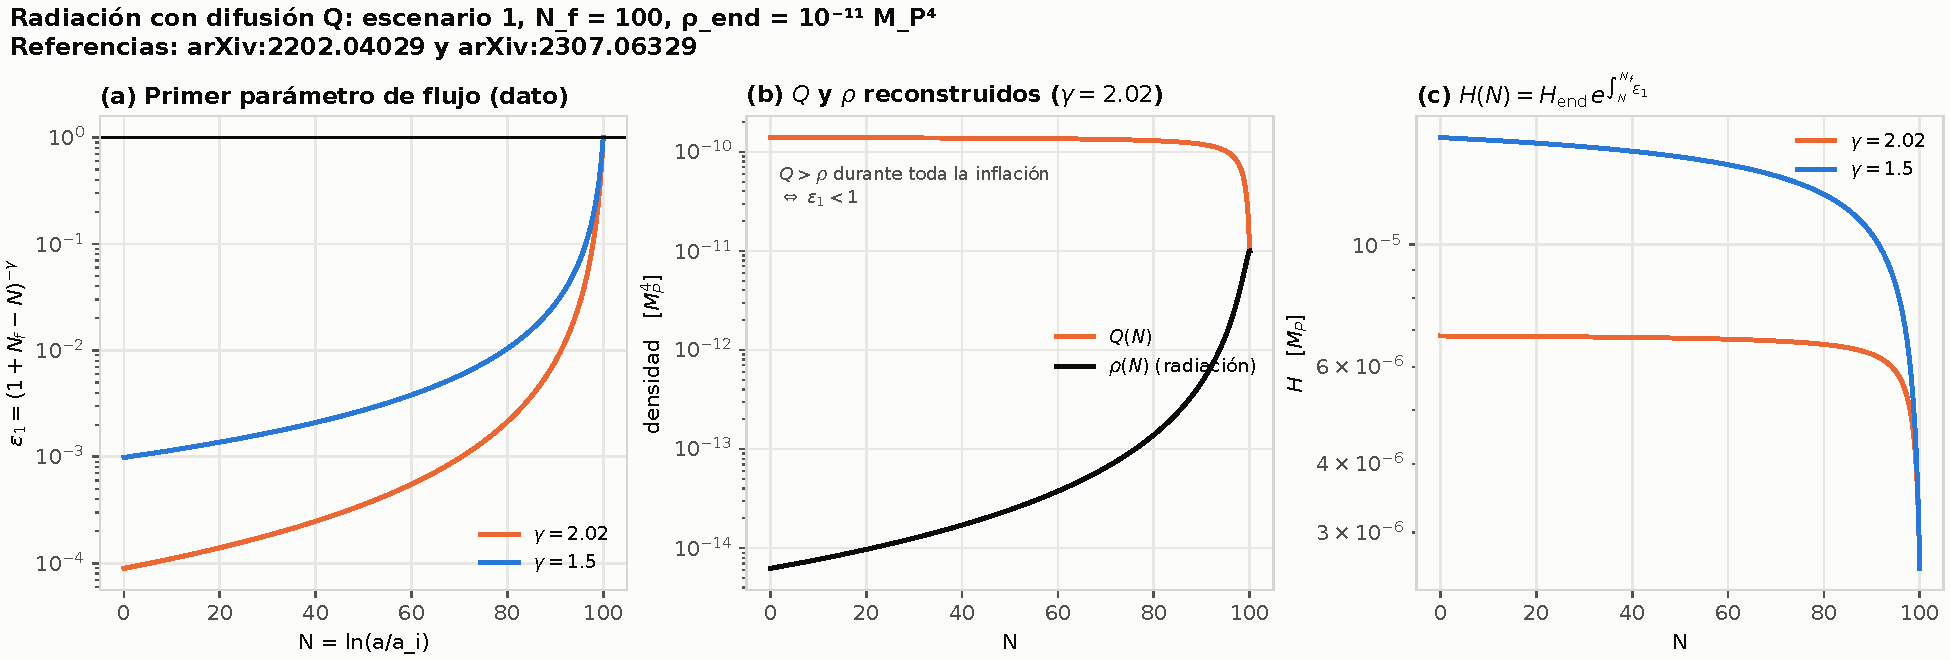
\includegraphics[width=\textwidth]{fig9_fondo_leon.pdf}
\caption{Modelo de radiación con difusión Q \cite{leon22,piccirilli23}, escenario 1 ($N_f=100$, $\rho_{\rm end}=10^{-11}\MP^4$). (a) $\epsilon_1(N)$ (dato) para $\gamma=2.02$ y $1.5$. (b) $Q$ y $\rho$ reconstruidos para $\gamma=2.02$: $Q>\rho$ mientras dura la inflación y se igualan al final. (c) $H(N)$. Generada por \texttt{make\_figures\_leon.py}.}
\label{fig:fondoleon}
\end{figure}

\subsection{Consecuencia para el espectro tensorial}
\label{sec:leonPT}

El resultado analítico de la sección~\ref{sec:tensores} (la ecuación de los modos es la de RG, con $X=0$) se aplica sin cambios, porque solo usa que $Q$ es escalar y que $T^i{}_j$ no tiene parte TT. El código de los modos (\texttt{modes.py}) es el mismo; cambia solo el fondo, que ahora sale de \eqref{eq:leonrec}. El término de masa $X$, calculado con $\rho$, $Q$, $H$ y la derivada numérica de $\ln H$ (sin suponerlo nulo), vale a lo sumo $2.5\times10^{-10}H^2$ para $N\le N_{\rm end}-0.5$.

El punto importante es que $P_T$ depende solo de $H(N)$ y $\epsilon_1(N)$, y con \eqref{eq:leonrec} esas funciones son las de \emph{cualquier} inflatón de RG que las reproduzca. Se comprobó: con $\dd\phi/\dd N=-\sqrt{2\epsilon_1}$ y $V=(3-\epsilon_1)H^2$ (las relaciones estándar de RG) se reconstruye un potencial $V(\phi)$, se integra la ecuación de Klein--Gordon de RG con él desde las mismas condiciones iniciales (un camino de código distinto), y sale el mismo $H(N)$ ($\max|\Delta\ln H|=8\times10^{-7}$) y el mismo $P_T$ (diferencia relativa $\sim10^{-10}$ en $N_*=50,60$ y $\le1.1\times10^{-6}$ en los 28 modos que alcanzan $q=10^{-3}$ de la figura~\ref{fig:PTleon}a; los otros dos se evalúan al final y se rotulan aparte). \emph{Dicho de otro modo: con el modelo de radiación con difusión Q \cite{leon22,piccirilli23} no existe una diferencia UG--RG en el sector tensorial a igual $H(N)$}; la diferencia entre marcos está en cuáles historias $H(N)$ se realizan (con $Q$ y radiación, o con un potencial) y en el sector escalar.

\subsection{Resultados}
\label{sec:leonres}

\begin{table}[t]
\centering\small
\renewcommand{\arraystretch}{1.2}
\begin{tabular}{@{}llrrrrrr@{}}
\toprule
Escenario & $N_*$ & $\epsilon_1$ & $P_T$ & $n_T$ & $A_s^{\rm PL}$ & $r_{\rm PL}$ & $n_{s,{\rm std}}$\\
\midrule
1, $\gamma=2.02$ & 50 & $3.6\times10^{-4}$ & $9.26\times10^{-12}$ & $-7.2\times10^{-4}$ & $1.63\times10^{-9}$ & $5.7\times10^{-3}$ & 0.960\\
1, $\gamma=2.02$ & 57 & $2.7\times10^{-4}$ & $9.30\times10^{-12}$ & $-5.5\times10^{-4}$ & $2.12\times10^{-9}$ & $4.4\times10^{-3}$ & 0.965\\
1, $\gamma=2.02$ & 60 & $2.5\times10^{-4}$ & $9.32\times10^{-12}$ & $-5.0\times10^{-4}$ & $2.35\times10^{-9}$ & $4.0\times10^{-3}$ & 0.966\\
1, $\gamma=1.5$ & 60 & $2.1\times10^{-3}$ & $4.42\times10^{-11}$ & $-4.2\times10^{-3}$ & $1.32\times10^{-9}$ & $3.4\times10^{-2}$ & 0.971\\
3, Starobinsky & 60 & $1.9\times10^{-4}$ & $4.60\times10^{-12}$ & $-3.7\times10^{-4}$ & $1.55\times10^{-9}$ & $3.0\times10^{-3}$ & 0.968\\
3, cuadrático & 60 & $8.3\times10^{-3}$ & $1.63\times10^{-10}$ & $-1.7\times10^{-2}$ & $1.24\times10^{-9}$ & $0.13$ & 0.967\\
\bottomrule
\end{tabular}
\caption{Espectro tensorial con el modelo de radiación con difusión Q \cite{leon22,piccirilli23} (\texttt{resultados/leon/comparacion.csv}; hay filas adicionales para $N_*=50$ del escenario 3). $P_T$ y $n_T$ son resultados. $A_s^{\rm PL}=H^2/(8\pi^2\epsilon_1)$ (Eq.~41 de \cite{piccirilli23}), $r_{\rm PL}=P_T/P_\mathcal{R}$ con esa fórmula y $n_{s,{\rm std}}=1-2\epsilon_1-\epsilon_2$ dependen del sector escalar, que no está derivado. Planck: $A_s=2.10\times10^{-9}$.}
\label{tab:leon}
\end{table}

\begin{figure}[t]
\centering
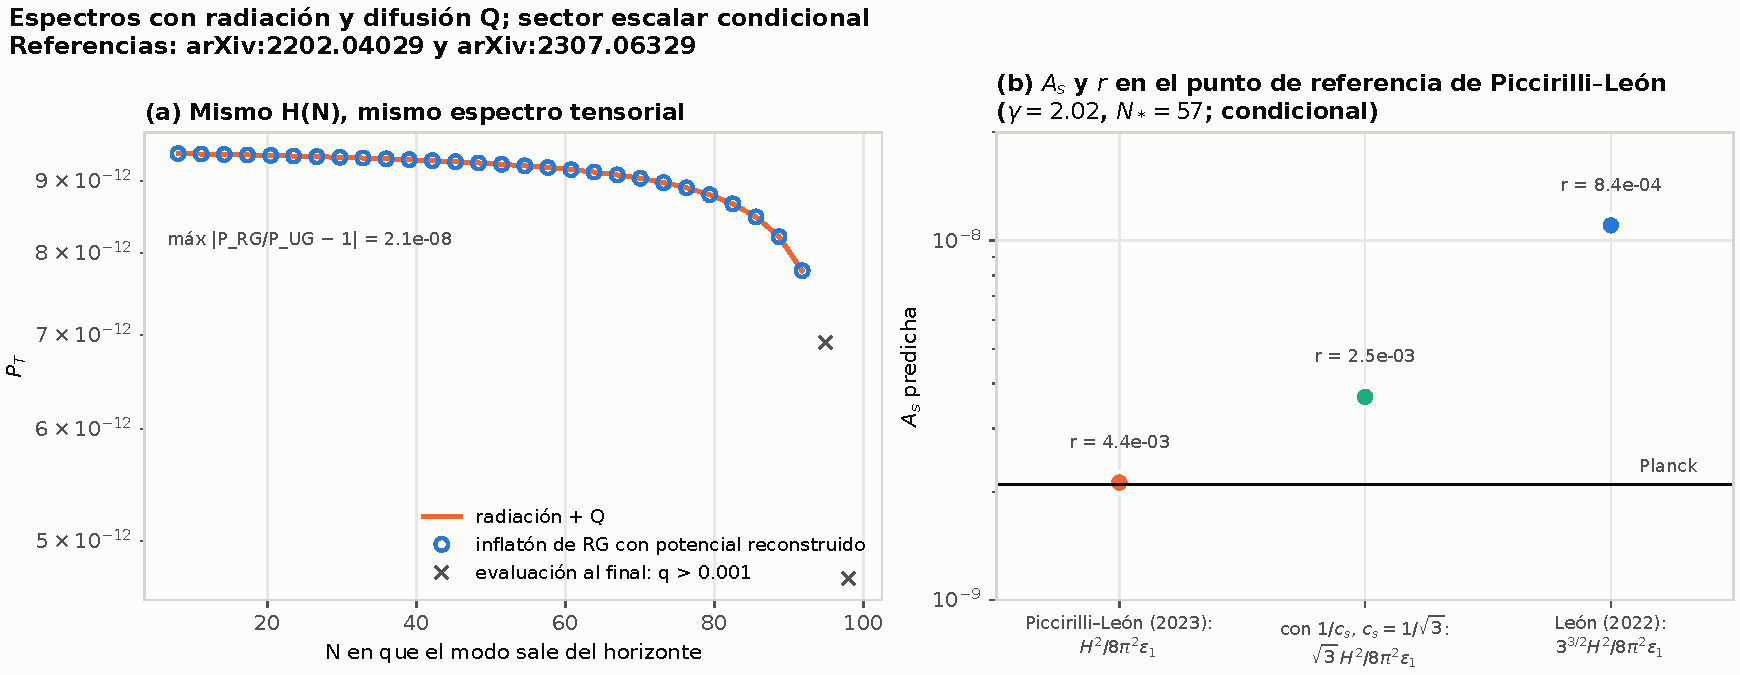
\includegraphics[width=\textwidth]{fig10_leon_PT_As.pdf}
\caption{(a) $P_T$ de los modos con el fondo de radiación más $Q$ (línea) y con el inflatón de RG de potencial reconstruido (círculos): mismo $H(N)$, mismo espectro. (b) $A_s$ predicha y $r$ en el punto de referencia de \cite{piccirilli23} ($\gamma=2.02$, $N_*=57$) según tres fórmulas escalares, todas condicionales. Generada por \texttt{make\_figures\_leon.py}.}
\label{fig:PTleon}
\end{figure}

La tabla~\ref{tab:leon} y la figura~\ref{fig:PTleon} resumen. Para el escenario 1 con $\gamma=2.02$ y $N_*=57$ (es decir, $N=43$ e-folds desde el inicio, el punto que \cite{piccirilli23} marca como consistente con los datos), el fondo da $P_T=9.3\times10^{-12}$, $n_T=-5.5\times10^{-4}$ y, con la fórmula de \cite{piccirilli23}, $A_s=2.12\times10^{-9}$, un $1.1\%$ por encima de Planck sin ajustar nada. Que $A_s$ salga en el valor de Planck cuando $\rho_{\rm end}$ y $N_f$ están fijos es un control de la implementación (\ref{sec:leoncontroles}). El valor $\gamma=1.5$, que \cite{piccirilli23} descarta con los datos de $n_s$ y $A_s$, da acá, a $N_*=60$, una $A_s$ un $37\%$ menor que la de Planck. Los espectros son casi planos en $k$ con una pendiente roja: para $\gamma=2.02$, $P_T$ vale $9.32\times10^{-12}$ en el modo que sale $60$ e-folds antes del final y $9.26\times10^{-12}$ en el que sale $50$ antes, con $n_T\approx-2\epsilon_1$.

\subsection{El mapeo del escenario 3 y el desfasaje de normalización}
\label{sec:leonmapeo}

CL7 compara únicamente la razón $P_T(N_*=60)/P_T(N_*=50)$ del mapeo con la de RG numérico, con $H$ igual al final. La discrepancia de esa razón es menor que $0.3\%$; no es un barrido de toda la forma. Los offsets absolutos conservados son de $23$--$29\%$. El criterio absoluto inicial de $10\%$ falló y se sustituyó por un criterio exploratorio de $3\%$ para la razón, después de observar el resultado. La explicación histórica en términos de acumulación de $\ln H$ y $\epsilon_V-\epsilon_H$ no está comprobada por un diagnóstico conservado que aísle esa causa.

\subsection{Controles}
\label{sec:leoncontroles}

Los siete controles de \texttt{checks\_leon.py} pasan: (CL1) la continuidad de radiación integrada numéricamente con el $Q(N)$ de la reconstrucción reproduce $\rho$, $H$ y $\epsilon_1$ a $1.7\times10^{-8}$ (escenarios 1 y 3); (CL2) $H^2$, $\rho$ y $Q$ del escenario 1 coinciden con las expresiones cerradas de \cite{piccirilli23} (Eqs.~46--48) a $3\times10^{-11}$; (CL3) el término de masa $X/H^2$ es $\le2.5\times10^{-10}$; (CL4) el inflatón de RG con el potencial reconstruido reproduce $H(N)$ y $P_T$; (CL5) $P_T$ coincide con el desarrollo de slow-roll de \cite{martin14} a segundo orden, con el mismo criterio de la sección~\ref{sec:controlesstaro}; (CL6) $A_s$ en el punto de \cite{piccirilli23} está a $1.1\%$ de Planck; (CL7) la razón $P_T(60)/P_T(50)$ del escenario 3 coincide con la de RG numérico a $\lesssim0.3\%$.

Dos cosas se ajustaron o se dejaron fuera \emph{después} de ver un resultado. CL1 se restringió a los escenarios 1 y 3, porque en el 2 la densidad $\rho$ llega a $\sim10^{-140}$ y la integración directa ensayada pierde precisión por cancelación (se obtiene de restar cantidades de orden uno; el condicionamiento crece como $\ee^{4N}$, y por eso \cite{leon22} grafica $\rho$ en escala logarítmica); no se probaron formulaciones reescaladas o logarítmicas; para ese escenario se conserva solo la reconstrucción desde $\epsilon_1$. CL7 se planteó primero como $|P_T^{\rm RG}/P_T^{\rm mapa}-1|\le10\%$, criterio fijado antes de correr, y \emph{falló} ($+23\%$ a $+29\%$); se reemplazó por un criterio exploratorio del 3\% sobre la razón entre dos pivotes, sin probar toda la forma y el desfasaje absoluto pasó a ser un resultado (subsección~\ref{sec:leonmapeo}).

\subsection{El sector escalar y $r$}
\label{sec:leonescalar}

El sector escalar no se derivó. Se calculó $A_s$ y $r$ con tres fórmulas alternativas para $P_\mathcal{R}$, todas condicionales: la de \cite{piccirilli23}, $H^2/(8\pi^2\epsilon_1)$; la de \cite{leon22} tal como está impresa (Eq.~66), con un factor $3^{3/2}$ adicional; y una tercera que corresponde a mi hipótesis sobre el origen de ese factor ($P_\mathcal{R}=H^2/(8\pi^2\epsilon_1c_s)$ con $c_s^2=1/3$, sin verificar contra el texto de \cite{garriga99}). En el punto de referencia ($\gamma=2.02$, $N_*=57$) resultan $A_s=2.12$, $11.0$ y $3.67$ (en unidades de $10^{-9}$) y $r=4.4\times10^{-3}$, $8.4\times10^{-4}$ y $2.5\times10^{-3}$, respectivamente. Solo la primera reproduce el valor de Planck, pero eso \emph{no} establece que sea la correcta: los parámetros de \cite{piccirilli23} se eligieron con esa fórmula, de modo que la consistencia con los datos es circular. Lo que sí muestra es que el factor $3^{3/2}$ de \cite{leon22} no es un detalle: con él, el punto de referencia queda $5$ veces por encima de $A_s$ (y $r$, cinco veces más chico). Resolver el factor requiere derivar el sector escalar, y sigue abierto (sección~\ref{sec:abiertos}).

CL6 admite un desvío relativo del $10\%$; el obtenido es $+1.0816\%$, aproximadamente $1.1\%$.

\section{Discusión y conclusiones}
\label{sec:discusion}

Esta última sección junta lo que se puede afirmar y lo que no. Está escrita para que el lector pueda decidir con qué está de acuerdo, así que insiste más en los puntos donde se podría discrepar que en los resultados.

\subsection{Qué se ha establecido}

El resultado analítico es que, sobre un fondo FLRW plano con un inflatón y bajo la hipótesis de que la materia no aporta tensión anisótropa TT, la ecuación de los modos tensoriales en UG, incluso con difusión, es la de RG (ecuación \eqref{eq:modok}), y que su acción cuadrática lo es también (ecuación \eqref{eq:S2TT}), esta última como hipótesis explícita de la realización efectiva (la ecuación de propagación no fija por sí sola la normalización cuántica), y que la difusión $Q$ y la constante de integración $\Lambda_0$ entran en el espectro tensorial únicamente a través de la función $H(t)$ del fondo. La argumentación distingue la ecuación lineal y una expansión formal condicionada, una a nivel de las ecuaciones de campo (el multiplicador es un escalar y por lo tanto pura traza, y el vínculo se cumple sin condiciones sobre un tensor sin traza a primer orden) y otra a nivel de la acción (el término del vínculo a segundo orden, $+\Lb a^3h_{ij}^2/4\kap$, cancela exactamente el término de masa que dejarían los otros dos aportes). Ambas coinciden con lo que la literatura afirma sin derivarlo del todo \cite{basak16,cho15,fabris22,barvinsky19}. De lo derivado a mano, la ecuación de los tensores a primer orden se verificó con álgebra simbólica (sección~\ref{sec:simbTT}); la acción a segundo orden y la cancelación del vínculo no, y hay un coeficiente (el del término de gradiente de la acción) que se fijó por consistencia y no por derivación.

El resultado numérico es que, para un inflatón y una difusión $Q(N)=Q_i\ee^{-\gamma N}$ con $Q_i/V_i=0.1$ y $\gamma=0.1$, y con las mismas condiciones iniciales en ambos modelos, la diferencia entre el espectro tensorial de UG y el de RG depende del potencial y del criterio de comparación (secciones~\ref{sec:resultados} y~\ref{sec:potenciales}). Con el potencial cuadrático, a igual $k$ comóvil UG es entre un 8.6\% y un 65.6\% menor que RG, pero a igual número de e-folds antes del final de cada inflación es un 50\% \emph{mayor}: el signo no es una propiedad de UG. Con el potencial de Starobinsky la reducción es $9.6$--$9.8\%$ a igual $N_*$ y $5.3$--$20.4\%$ a igual $k$, y las diferencias de $n_T$ son pequeñas (no se evaluó su detectabilidad instrumental). Con el modelo de radiación con difusión Q \cite{leon22,piccirilli23} (radiación más $Q$, sección~\ref{sec:leon}) no hay diferencia tensorial a igual $H(N)$: $P_T$ es el de RG con ese $H(N)$. Las diferencias de las secciones~\ref{sec:resultados} y~\ref{sec:potenciales} no son artefactos numéricos y se explican por el fondo: el cociente numérico coincide con la fórmula estándar de RG evaluada con el $H$ y el $\epsilon_1$ de UG con máximo $2.80\times10^{-5}$ en los modos juzgados del cuadrático (muestra de C3.4; se excluyen los puntos que no satisfacen su criterio slow-roll). El código reproduce además, con una precisión muy por debajo de la diferencia UG--RG, el límite estándar de RG (de Sitter exacto, desarrollo de slow-roll a segundo orden, las predicciones conocidas de $\phi^2$).

\subsection{De qué decisiones depende la magnitud}
\label{sec:decisiones-dep}

Lo anterior se dice para \emph{estos} parámetros, y es importante entender cuánto de la magnitud de la diferencia es una propiedad de UG y cuánto es una propiedad de la parametrización elegida. La respuesta es que casi toda la magnitud es de lo segundo.

La decisión más fuerte es la de $\Lambda_0$. Pedir las mismas condiciones iniciales ($\phi_i$, $\dot\phi_i$, $H_i$) en RG y en UG fija $\Lambda_0=-Q_i$, negativa y comparable a la densidad de energía total al inicio ($Q_i$ es el 10\% de $V(\phi_i)$). Como mostró la figura~\ref{fig:fondo}, eso hace que $3H^2=\rho_\phi-Q_i+Q(N)$ pierda energía respecto de RG durante toda la inflación y que, al final, esa constante negativa sea comparable a $\rho_\phi$: la inflación de UG (con el potencial cuadrático) termina en $\epsilon_1=1$, aunque el parámetro del potencial desnudo sea pequeño, y $H$ cae mucho más rápido que en RG. En Starobinsky el presupuesto energético al final es distinto, pero no se aisló la causa variando la constante. Una elección alternativa igualmente razonable, $\Lambda_0=0$ con los mismos $(\phi_i,\dot\phi_i)$, daría $H_i^{\rm UG}=\sqrt{(\rho_i+Q_i)/3}>H_i^{\rm RG}$ y un $H$ mayor en UG mientras $Q$ es apreciable; a partir de \eqref{eq:H2UG} cabe esperar que el signo de la diferencia en $P_T$ sea el opuesto en la primera parte del rango de $k$. No se calculó, y no se afirma. Lo que sí se calculó (sección~\ref{sec:resultadosN}) es que, incluso con $\Lambda_0=-Q_i$, el signo cambia según se compare a igual $k$ o a igual $N_*$: la magnitud y el signo de la diferencia dependen de decisiones que no fija la teoría.

Otras decisiones actúan más suavemente. La forma de $Q(N)$ y los valores de $Q_i/V_i$ y $\gamma$ son elecciones fenomenológicas; un barrido exploratorio preliminar en el notebook (no verificado y no registrado como resultado) sugiere que el cociente UG/RG varía fuertemente con $Q_i/V_i$. La velocidad inicial de slow-roll de RG produce el salto inicial de $\epsilon_1$ de UG, que es una consecuencia de imponer las mismas condiciones iniciales y no una propiedad de la teoría. La duración de la inflación de UG ($100$ e-folds) se fijó por la literatura, y hace que RG dure más ($161.8$ con el potencial cuadrático y $386.7$ con el de Starobinsky). Y el mismo $k$ no corresponde a la misma escala observacional en los dos modelos; por eso la comparación principal es a igual $N_*$ (sección~\ref{sec:igualN}). Es una convención ilustrativa, no una identificación de la misma escala observacional: identificar el mismo $k_*$ físico exige la historia posterior (el recalentamiento) y la normalización de $a$, que no se modelan.

Lo que sí es robusto, siempre que la derivación sea correcta, es el \emph{mecanismo}: $P_T$ depende de $Q$ solo a través de $H(t)$, de modo que cualquier efecto de la difusión sobre el espectro tensorial se lee en el fondo. La cantidad de efecto es, en cambio, una predicción del modelo de $Q$ que se elija, y no de UG como tal.

\subsection{Supuestos que sostienen el resultado analítico}
\label{sec:supuestos}

Hay varios puntos en los que el lector podría legítimamente discrepar, y conviene enumerarlos.

El primero y más importante es la hipótesis sobre la materia. La sección~\ref{sec:acoplamiento} la precisa para el caso de un solo campo: si $Q$ intercambia energía con el inflatón y es covariante, para un escalar canónico y una difusión local especificada como $Q(\phi)$, las ecuaciones de UG pueden reescribirse como las de RG con $V_{\rm eff}=V+Q(\phi)+\Lambda_0$ (sobre la rama reconstruida, si se parte de $Q(N)$); y si además se impone $\delta Q=0$ en el marco especificado y la perturbación del inflatón es inhomogénea, resulta $\dot Q=0$. Ninguna de las dos afirmaciones es una equivalencia o una prohibición general (sección~\ref{sec:acoplamiento}). La conclusión de que la acción cuadrática de los tensores es la de RG usa que el tensor energía-impulso no tiene parte TT a primer orden, \eqref{eq:TTmateria}, y que el aporte de la materia a la acción a segundo orden es el estándar, \eqref{eq:Sm2}. La ausencia de parte TT a primer orden no justifica por sí sola el aporte de materia a segundo orden con intercambio de energía. Pero, como se dijo en el recuadro de la sección~\ref{sec:difusionQ}, la difusión $Q$ variable exige que la materia \emph{no} sea la de una acción covariante estándar, y no se sabe qué modificaciones concretas de la materia producen esa no conservación. Si el mecanismo microscópico detrás de $Q$ (por ejemplo, los efectos de \cite{josset17,perez19}) generara una tensión anisotrópica, o modificara la acción de la materia a segundo orden en $h_{ij}$, los tensores podrían verse afectados de un modo que este análisis no captura. Es un supuesto compartido con las demás referencias que tratan tensores con difusión \cite{fabris22}.

El segundo es el tratamiento del vínculo a segundo orden. La derivación fija $g_{00}=-1$ y deja que el multiplicador absorba la violación de segundo orden del volumen. Una alternativa es perturbar también el lapse a segundo orden, $N=1+\tfrac14h_{ij}^2$, de modo que el vínculo se cumpla exactamente; la diferencia entre ambas formulaciones multiplica la ecuación de fondo de la componente temporal, y cabe esperar que la acción en capa sea la misma, pero ese argumento no se desarrolló en el trabajo y sería bueno comprobarlo con álgebra simbólica. La observación de la sección~\ref{sec:accion2} sobre la parametrización exponencial cubre una elección relacionada, no esta.

El tercero es que el coeficiente del término de gradiente de \eqref{eq:S2TT}, $-\tfrac14a(\partial_kh_{ij})^2$, no se derivó sino que se tomó como estándar y se contrastó por consistencia con la ecuación de campo. Y el cuarto es más general: la derivación es a mano, y algunos pasos estándar (por ejemplo, la forma ADM de Einstein--Hilbert) no se contrastaron con el texto de un libro. La verificación simbólica cubre solo la ecuación de los tensores a primer orden y algunas identidades del fondo y del acoplamiento de $Q$ (sección~\ref{sec:acoplamiento}).

Hay además cosas que no se consideran. Se trabaja a nivel lineal en el fondo homogéneo, de modo que no se estudian las ondas gravitacionales inducidas a segundo orden por las perturbaciones escalares (en UG el sector escalar tiene un gauge restringido y $\delta Q$ podría contribuir), ni posibles correcciones al estado inicial de Bunch--Davies debidas a los mecanismos que generan $Q$.

\subsection{Lo que queda abierto}
\label{sec:abiertos}

La ausencia principal es el sector escalar, y con ella la relación tensor-escalar $r$, que es la cantidad observacionalmente relevante. Hay un problema específico en la literatura que este trabajo no resuelve pero que conviene describir, porque motivó el proyecto. El artículo de León \cite{leon22} da un espectro escalar (su Ec.~66) con un factor $3^{3/2}$ en el numerador, $P_\mathcal{R}=3^{3/2}H^2/(8\pi^2\MP^2\epsilon_1)$; el de Piccirilli y León \cite{piccirilli23}, que dice basarse en aquél, tiene la misma expresión sin ese factor (su Ec.~41), y luego adopta $r=16\,\epsilon_1$ (su Ec.~42) citando un trabajo que no contiene sector tensorial. Con el $P_\mathcal{R}$ de \cite{leon22} y el $P_T$ estándar, aritméticamente resultaría $r=16\epsilon_1/3^{3/2}\approx3.1\,\epsilon_1$, no $16\epsilon_1$. Esa observación, y una hipótesis sobre su origen (que $3^{3/2}$ podría venir de una velocidad del sonido $c_s^2=1/3$, aunque la expresión que recuerdo para un fluido con velocidad del sonido $c_s$, asociada a \cite{garriga99}, tiene $c_s^{-1}$, esto es $3^{1/2}$ y no $3^{3/2}$, y no la verifiqué contra el texto de ese artículo), son conjeturas mías que no se verificaron. Lo que este trabajo aporta a ese problema es la mitad tensorial: $P_T$ es el de RG evaluado con el $H$ de UG. La otra mitad, $P_\mathcal{R}$ con difusión, es una tarea pendiente.

Para el modelo con inflatón y $Q(\phi)$ el sector escalar tampoco está derivado: si la equivalencia con RG con $V_{\rm eff}$ fuese correcta a nivel de perturbaciones valdrían las fórmulas estándar, pero esa equivalencia se argumentó a mano y no se verificó (sección~\ref{sec:unescalar}). Y queda abierto el sector escalar en el marco $\delta Q=0$ con radiación, que es el de \cite{leon22,piccirilli23}; con el fondo de esa literatura, $A_s$ y $r$ dependen de una fórmula escalar no derivada, y el factor $3^{3/2}$ cambia $A_s$ por un factor cinco (sección~\ref{sec:leonescalar}). Otros puntos abiertos, en orden de prioridad sugerida: el escenario 2 del modelo de radiación con difusión Q \cite{leon22,piccirilli23}, que necesita $N_f\simeq370$ y una integración de precisión extendida (sección~\ref{sec:leon}), y una normalización del mapeo del escenario 3 que no acumule el error del final de la inflación; un barrido controlado de $Q_i$, $\gamma$ y $\phi_i$, y de la prescripción de $\Lambda_0$; la relación entre $k$ y la escala observacional, que requiere modelar el recalentamiento; la verificación simbólica de la acción a segundo orden y el contraste de los pasos estándar con los textos de referencia; y, por requisito del curso, el registro formal de los números y afirmaciones del trabajo con su procedencia y una segunda lectura independiente, hecha por alguien sin la historia de este trabajo.

\subsection{Conclusiones}

El trabajo intentó cerrar un hueco específico de la literatura sobre gravedad unimodular con difusión: partiendo de la acción con multiplicador de Lagrange, ¿cambia la ecuación de las ondas gravitacionales primordiales? La respuesta que se obtiene, con los supuestos explicitados arriba, es que no cambia: el vínculo unimodular no toca a los modos transversos y sin traza a primer orden, y a segundo orden su contribución a la acción se cancela exactamente con las demás, de modo que la difusión $Q$ solo llega al espectro tensorial a través del parámetro de Hubble. Los controles numéricos son consistentes con esa conclusión, aunque no la prueban de manera independiente.

Lo que sí se puede afirmar, además, es de naturaleza más práctica. El espectro tensorial en UG con difusión se calcula como en RG con el fondo de UG, y toda la información sobre $Q$ que llega al espectro está en $H(t)$; por lo tanto, medir $P_T$ (o acotar $r$) restringe la difusión $Q$ solo a través de su efecto sobre el fondo. Y cuánto restringe depende, como se vio, de decisiones de modelado (empezando por $\Lambda_0$, el potencial y el criterio de comparación) que la teoría no fija; en particular, para un escalar canónico con $Q(\phi)$ el efecto se reduciría a usar otro potencial, siempre que la equivalencia perturbativa se confirme (sección~\ref{sec:unescalar}). El mensaje central es entonces: a igual fondo, y bajo las hipótesis adoptadas, la propagación tensorial no distingue UG de RG; las diferencias de los ejemplos provienen del fondo y del criterio de comparación; el acoplamiento escalar y las fórmulas alternativas de $A_s$ son discusión condicionada. Quien lea este informe con ojo crítico debería decidir, en primer lugar, si le parecen aceptables los supuestos sobre la materia de la sección~\ref{sec:supuestos}; en segundo lugar, si la decisión de fijar el mismo $H_i$ en RG y en UG y de comparar a igual $N_*$ es la comparación que le interesa; y, en tercer lugar, si el marco de trabajo es el de un inflatón con $Q=Q(\phi)$ o el de $\delta Q=0$ con radiación, y si el siguiente paso es el sector escalar en ese marco o el barrido de parámetros.


\appendix
\section{Procedencia de las ecuaciones clave}
\label{ap:procedencia}
\sloppy

La tabla siguiente enlaza cada ecuación importante de este informe (primera columna) con su lugar en \texttt{derivation.md} (la derivación del proyecto, cuya numeración se conserva por las referencias cruzadas), su etiqueta de procedencia, la función del código que la implementa y el control que la ejerce. Las etiquetas son: P, álgebra propia (a mano); C, tomada de un artículo; E, estándar de libro de texto (no contrastada con las fuentes salvo donde se indica); S, supuesto o decisión. Una ``ec.\ n'' entre paréntesis sin más es la numeración de \texttt{derivation.md}. ``---'' significa que no hay implementación o control específico.

\small
\begin{longtable}{@{}L{2.0cm}L{2.4cm}L{1.0cm}L{5.2cm}L{2.7cm}@{}}
\toprule
\textbf{Ec.} & \textbf{\texttt{derivation.md}} & \textbf{Etiq.} & \textbf{Código} & \textbf{Control}\\
\midrule
\endfirsthead
\toprule
\textbf{Ec.} & \textbf{\texttt{derivation.md}} & \textbf{Etiq.} & \textbf{Código} & \textbf{Control}\\
\midrule
\endhead
\bottomrule
\endfoot
\eqref{eq:SUG}, \eqref{eq:vinculo} & (1.1), (1.4) & C & --- & ---\\
\eqref{eq:EinsteinUG} & (1.3) & C, P & --- & ---\\
\eqref{eq:lambdatraza}, \eqref{eq:trazafree} & (1.5), (1.6) & P & --- & ---\\
\eqref{eq:gradlambda} & (1.7) & P & --- & C3.1 (límite $Q$ cte)\\
\eqref{eq:Qdef} & (1.8), (1.9) & C & \texttt{background.py::Q\_of\_N, Qdot} & ---\\
\eqref{eq:FriedUG} & (2.6) & P & \texttt{hubble\_rg}, \texttt{hubble\_ug} & C3.1\\
\eqref{eq:H2UG} & (2.7) & P & \texttt{hubble\_ug} & C3.1, C3.2\\
\eqref{eq:HdotUG} & (2.8) & P & \emph{no se usa}; se contrasta & C3.2\\
\eqref{eq:contUG} & Continuidad (Sec.~2.4) & P & --- & ---\\
\eqref{eq:KGQ} & (2.9) & P, S & \texttt{quantities\_ug} & C3.1, C3.2\\
\eqref{eq:Lambda0} & (2.11) & P & \texttt{lambda0\_from\_initial} & C3.1\\
\eqref{eq:eps1UG} & (2.12) & P & --- (se calcula de $\dot H$) & C3.2\\
\eqref{eq:slowUG} & (2.14) & P, S & \texttt{initial\_state} ($\dot\phi_i$) & ---\\
\eqref{eq:Rijh}, \eqref{eq:GTT} & (3.4), (3.5) & P & --- & solo a mano\\
\eqref{eq:modo}, \eqref{eq:modok} & (3.8), (3.9) & P & \texttt{modes.py::mode\_rhs} & C1.1, C1.2, C3.3\\
\eqref{eq:modoconf} & (3.10), (3.11) & P & \texttt{mode\_rhs} & C1.1\\
\eqref{eq:fabris} & (3.12) & P, C & --- & solo a mano (cierra O3 a mano)\\
\eqref{eq:modoT} & (3.13) & P & --- & ---\\
\eqref{eq:vinculo2} & (4.1) & P & --- & ---\\
\eqref{eq:Slambda2}, \eqref{eq:cancel} & (4.5), (4.6) & P & \texttt{background.py::tensor\_mass\_term} & C3.5\\
\eqref{eq:S2TT} & (4.7) & P, E & --- & solo a mano; gradiente E\\
\eqref{eq:S2v} & (4.8) & P, S & --- & C1.1 (indirecto)\\
\eqref{eq:modoX} & (no numerada; n1) & P & \texttt{mode\_rhs} & C3.3, C3.5\\
\eqref{eq:modoN} & (no numerada; n2) & P & \texttt{mode\_rhs} & C3.3\\
\eqref{eq:BDwkb} & (no numerada; n5) & E, S & \texttt{modes.py::bunch\_davies\_ic} & C1.1, C2\\
\eqref{eq:PTdef}, \eqref{eq:PTcode} & fila P2 corregida; n4 & E, S & \texttt{modes.py::tensor\_power} & C1.1, C1.2\\
\eqref{eq:PTRG}, \eqref{eq:PTNLO} & --- & E, C & \texttt{checks.py} (comparación) & C1.1--C1.3\\
\eqref{eq:PTUG}, \eqref{eq:cociente} & --- & P (consecuencia) & --- & C3.4\\
\end{longtable}
\normalsize

Las ecuaciones ``no numeradas'' n1, n2, n4 y n5 son pasos que el código usa y que no estaban escritos en \texttt{derivation.md}; se documentan en \texttt{PROVENANCE.md} (sec.~9.3) y se incorporan a este informe (secciones~\ref{sec:normalizacion} y~\ref{sec:numerico}). Queda pendiente decidir si se agregan a \texttt{derivation.md}.

\section{Detalles de álgebra}
\label{ap:algebra}

Este apéndice desarrolla los pasos de la sección~\ref{sec:tensores} y de la sección~\ref{sec:numerico} que se saltearon en el texto principal. Todo es álgebra propia hecha a mano, con las verificaciones de consistencia indicadas en cada caso, y no se contrastó con álgebra simbólica.

\subsection{El tensor de Ricci a primer orden}

Con la métrica $g_{00}=-1$, $g_{0i}=0$, $g_{ij}=a^2(\delta_{ij}+h_{ij})$ y los símbolos de Christoffel \eqref{eq:Gammah}, se calcula $R_{ij}=\partial_\mu\Gamma^\mu_{ij}-\partial_j\Gamma^\mu_{i\mu}+\Gamma^\mu_{\mu\lambda}\Gamma^\lambda_{ij}-\Gamma^\mu_{j\lambda}\Gamma^\lambda_{i\mu}$ término a término. Los Christoffel se obtienen de $\Gamma^0_{ij}=\tfrac12\partial_tg_{ij}=a^2[H(\delta+h)_{ij}+\tfrac12\dot h_{ij}]$ y de $\Gamma^i_{0j}=\tfrac12g^{ik}\partial_tg_{kj}=H\delta_{ij}+\tfrac12\dot h_{ij}+\mathcal O(h^2)$, ya que $g^{ik}=a^{-2}(\delta-h)_{ik}$ y $(\delta-h)(\delta+h)=\delta+\mathcal O(h^2)$.

\paragraph{Primer término.} $\partial_\mu\Gamma^\mu_{ij}=\partial_t\Gamma^0_{ij}+\partial_k\Gamma^k_{ij}$. Derivando,
\begin{equation}
\partial_t\Gamma^0_{ij}=2a^2H\big[H(\delta+h)+\tfrac12\dot h\big]+a^2\big[\dot H(\delta+h)+H\dot h+\tfrac12\ddot h\big]=a^2\big[(2H^2+\dot H)(\delta+h)_{ij}+2H\dot h_{ij}+\tfrac12\ddot h_{ij}\big],
\end{equation}
y $\partial_k\Gamma^k_{ij}=\tfrac12\big(\partial_k\partial_ih_{kj}+\partial_k\partial_jh_{ki}-\nabla^2h_{ij}\big)=-\tfrac12\nabla^2h_{ij}$ por la transversalidad.

\paragraph{Segundo término.} $\partial_j\Gamma^\mu_{i\mu}=\partial_j\partial_i\ln\sqrt{-g}=0$, porque $\ln\sqrt{-g}=3\ln a+\mathcal O(h^2)$.

\paragraph{Tercer término.} $\Gamma^\mu_{\mu 0}=3H$ y $\Gamma^\mu_{\mu k}=\partial_k\ln\sqrt{-g}=0$, de modo que $\Gamma^\mu_{\mu\lambda}\Gamma^\lambda_{ij}=3H\,\Gamma^0_{ij}=3Ha^2\big[H(\delta+h)_{ij}+\tfrac12\dot h_{ij}\big]$.

\paragraph{Cuarto término.} Contribuyen $(\mu,\lambda)=(0,k)$ y $(k,0)$ a primer orden (el término $(k,l)$ es de segundo orden): $\Gamma^\mu_{j\lambda}\Gamma^\lambda_{i\mu}=2\,\Gamma^0_{jk}\Gamma^k_{i0}=2a^2\big[H^2(\delta+h)_{ij}+H\dot h_{ij}\big]$.

\paragraph{Suma.} Los coeficientes de $(\delta+h)_{ij}$ suman $(2H^2+\dot H)+3H^2-2H^2=\dot H+3H^2$; los de $\dot h_{ij}$ suman $2H+\tfrac32H-2H=\tfrac32H$; y queda $\tfrac12\ddot h_{ij}$ y $-\tfrac12\nabla^2h_{ij}$. Es decir,
\begin{equation}
R_{ij}=a^2(\dot H+3H^2)(\delta_{ij}+h_{ij})+\tfrac12a^2\big(\ddot h_{ij}+3H\dot h_{ij}\big)-\tfrac12\nabla^2h_{ij},
\end{equation}
que es \eqref{eq:Rijh}. Para el tensor mixto, $R^i{}_j=g^{ik}R_{kj}=a^{-2}(\delta-h)_{ik}R_{kj}=(\dot H+3H^2)\delta_{ij}+\tfrac12(\ddot h_{ij}+3H\dot h_{ij})-\tfrac12\nabla^2h_{ij}/a^2$, y con $R=6(\dot H+2H^2)$ (sin perturbación a primer orden) se obtiene \eqref{eq:GTT}: $G^i{}_j=R^i{}_j-\tfrac12R\,\delta^i_j$ tiene el coeficiente $\dot H+3H^2-3\dot H-6H^2=-(2\dot H+3H^2)$ en la parte de fondo.

\subsection{Cambio de variable a la forma de Fabris et al.}

Sustituyendo $h=\hat h/a^2$, $\dot h=(\dot{\hat h}-2H\hat h)/a^2$ y $\ddot h=(\ddot{\hat h}-4H\dot{\hat h}-2\dot H\hat h+4H^2\hat h)/a^2$ en \eqref{eq:modok} y multiplicando por $a^2$:
\begin{equation}
\ddot{\hat h}-4H\dot{\hat h}-2\dot H\hat h+4H^2\hat h+3H\dot{\hat h}-6H^2\hat h+\frac{k^2}{a^2}\hat h=\ddot{\hat h}-H\dot{\hat h}-2(\dot H+H^2)\hat h+\frac{k^2}{a^2}\hat h=0,
\end{equation}
que es \eqref{eq:fabris}.

\subsection{La ecuación en el tiempo unimodular}

Con $\dd T=a^3\dd t$ resulta $\tfrac{\dd}{\dd t}=a^3\tfrac{\dd}{\dd T}$ y $H=\dot a/a=a^2a_T$. Entonces $\dot h=a^3h_T$ y $\ddot h=a^3\tfrac{\dd}{\dd T}(a^3h_T)=a^6h_{TT}+3a^5a_Th_T$; con $3H\dot h=3a^5a_Th_T$, \eqref{eq:modok} queda $a^6h_{TT}+6a^5a_Th_T+(k^2/a^2)h=0$, y dividiendo por $a^6$ se obtiene \eqref{eq:modoT}.

\subsection{La acción a segundo orden}

\paragraph{Curvatura extrínseca.} Con lapse $N=1$, la métrica espacial es $\gamma_{ij}=a^2M_{ij}$ con $M=\delta+h$, y la curvatura extrínseca es $K^i{}_j=\tfrac12\gamma^{ik}\dot\gamma_{kj}=H\delta^i_j+\tfrac12(M^{-1}\dot h)_{ij}$. Como $\mathrm{tr}\,h=0$, $\mathrm{tr}(M^{-1}\dot h)=\tfrac{\dd}{\dd t}\ln\det M=\tfrac{\dd}{\dd t}\mathrm{tr}\ln(1+h)=-\tfrac12\tfrac{\dd}{\dd t}h_{ij}^2$, de modo que $K=3H-\tfrac14\tfrac{\dd}{\dd t}h_{ij}^2$. Con $A\equiv M^{-1}\dot h$:
\begin{align}
K^i{}_jK^j{}_i&=3H^2+H\,\mathrm{tr}A+\tfrac14\mathrm{tr}(A^2)=3H^2-\tfrac12H\tfrac{\dd}{\dd t}h_{ij}^2+\tfrac14\dot h_{ij}^2+\mathcal O(h^3),\\
K^2&=9H^2+3H\,\mathrm{tr}A+\mathcal O(h^4)=9H^2-\tfrac32H\tfrac{\dd}{\dd t}h_{ij}^2+\mathcal O(h^4),
\end{align}
y la diferencia es $K^i{}_jK^j{}_i-K^2=-6H^2+H\tfrac{\dd}{\dd t}h_{ij}^2+\tfrac14\dot h_{ij}^2$, que es \eqref{eq:Kh}.

\paragraph{Multiplicación por $\sqrt\gamma$ e integración por partes.} Con $\sqrt\gamma=a^3(1-\tfrac14h_{ij}^2)$,
\begin{equation}
\sqrt\gamma\,(K_{ij}K^{ij}-K^2)=a^3\Big[-6H^2+\tfrac32H^2h_{ij}^2+H\tfrac{\dd}{\dd t}h_{ij}^2+\tfrac14\dot h_{ij}^2\Big].
\end{equation}
Integrando por partes, $\int a^3H\tfrac{\dd}{\dd t}h_{ij}^2\,\dd t=-\int\tfrac{\dd}{\dd t}(a^3H)\,h_{ij}^2\,\dd t=-\int(3a^3H^2+a^3\dot H)\,h_{ij}^2\,\dd t$, y los coeficientes de $h_{ij}^2$ suman $\tfrac32H^2-3H^2-\dot H=-(\tfrac32H^2+\dot H)$: es \eqref{eq:KKh}.

\paragraph{Suma de los términos sin derivadas.} Con el factor $\frac{1}{2\kap}$ de $S_{EH}$, el aporte de \eqref{eq:KKh} es $\frac{a^3h_{ij}^2}{2\kap}\,[-\tfrac32H^2-\dot H]=\frac{a^3h_{ij}^2}{4\kap}[-3H^2-2\dot H]$. El de la materia \eqref{eq:Sm2} es $-\tfrac14a^3ph_{ij}^2=\frac{a^3h_{ij}^2}{4\kap}[-\kap p]$, y el del vínculo \eqref{eq:Slambda2} es $\frac{a^3h_{ij}^2}{4\kap}[\Lb]$. La suma es \eqref{eq:cancel}.

\subsection{La ecuación de modos con el término de masa}

Si se conserva el corchete de \eqref{eq:cancel} sin anularlo, $X\equiv-3H^2-2\dot H-\kap p+\Lb$, la parte de la lagrangiana sin derivadas es $\frac{a^3}{4\kap}X\,h_{ij}^2$, y la acción completa es
\begin{equation}
S=\frac{1}{8\kap}\int\dd t\,\dd^3x\,\Big[a^3\dot h_{ij}^2-a(\partial_kh_{ij})^2+2a^3X\,h_{ij}^2\Big].
\end{equation}
Para cada componente TT la ecuación de Euler--Lagrange es $\tfrac{\dd}{\dd t}(a^3\dot h)-a\nabla^2h-2a^3Xh=0$, es decir $\ddot h+3H\dot h-\nabla^2h/a^2-2Xh=0$, que en Fourier es \eqref{eq:modoX}. En tiempo conforme, con $\dot h=h'/a$ y $\ddot h=(h''-\mathcal Hh')/a^2$, se obtiene $h''+2\mathcal Hh'+(k^2-2Xa^2)h=0$, y con $v=ah$ (y $a''/a$ de la sección~\ref{sec:ecmodosnum}), $v''+(k^2-a''/a-2Xa^2)v=0$.

\subsection{Paso a la variable $N$}

Con $\tfrac{\dd}{\dd\eta}=aH\tfrac{\dd}{\dd N}$ y $w=\dd v/\dd N$, $v'=aHw$ y
\begin{equation}
v''=aH\,\frac{\dd}{\dd N}(aH\,w)=aH\,(aH)_N\,w+a^2H^2w_N=a^2H^2\big[(1-\epsilon_1)\,w+w_N\big],
\end{equation}
donde se usó $(aH)_N=aH\,(1+H_N/H)=aH\,(1-\epsilon_1)$. Sustituyendo en $v''+(k^2-a''/a-2Xa^2)v=0$ con $a''/a=a^2H^2(2-\epsilon_1)$ y dividiendo por $a^2H^2$ se obtiene \eqref{eq:modoN}.

\section{Fuentes y nivel de lectura}
\label{ap:fuentes}

Casi todo el sustento bibliográfico de este informe proviene de una etapa de literatura previa, cuyos detalles están en \texttt{PROVENANCE.md}. Lo que sigue dice, para cada fuente, cuánto se leyó realmente, porque una afirmación apoyada en un resumen no tiene el mismo peso que una apoyada en el texto. Los niveles son: \textbf{texto parcial}, se extrajo el texto del PDF y se leyeron las ecuaciones y secciones indicadas (no el artículo entero); \textbf{resumen}, solo se verificaron el resumen y los metadatos, de modo que lo que se dice de ese artículo es lo que su resumen afirma y debería releerse antes de usarlo como sustento; \textbf{no leído}, no se accedió al texto (de pago o no descargado). Las citas textuales que aparecen en este informe son traducciones libres, hechas por quien escribió el texto, de los originales en inglés.

\begingroup\small
\renewcommand{\arraystretch}{1.2}
\begin{longtable}{@{}L{4.2cm}L{2.6cm}L{7.2cm}@{}}
\toprule
\textbf{Fuente} & \textbf{Nivel} & \textbf{Qué se toma}\\
\midrule
\endhead
León (2022) \cite{leon22} & texto parcial & Ecs.\ de fondo con $Q$ (9)--(12), (15), (57); espectro escalar (66); $N_f$; ausencia de sector tensorial\\
Piccirilli y León (2023) \cite{piccirilli23} & texto parcial & Ecs.\ (38), (40)--(42), (44); $N_f=100$; $r=16\epsilon_1$ sin derivación\\
Bengochea et al.\ (2023) \cite{bengochea23} & texto parcial & Acción (2.1), ecuaciones (2.5)--(2.15), tiempo unimodular (3.12), invariancia de gauge (5.10)\\
Padilla y Saltas (2015) \cite{padilla15} & texto parcial & Acción con multiplicador; equivalencia clásica con RG; acción de Henneaux--Teitelboim\\
Ellis et al.\ (2011, 2014) \cite{ellis11,ellis14} & resumen (+ búsqueda negativa de tensores) & Ecuaciones sin traza; no resuelven el valor de $\Lambda$; inflación ``como de costumbre''\\
Carballo-Rubio et al.\ (2022) \cite{carballo22} & texto parcial & Teoría lineal: WTDiff frente a Fierz--Pauli\\
Basak et al.\ (2016) \cite{basak16} & texto parcial & Resumen y conclusiones: tensores no afectados por el vínculo\\
Gao et al.\ (2014) \cite{gao14} & texto parcial & Restricción del gauge escalar; solo sector escalar\\
Cho y Singh (2015) \cite{cho15} & texto parcial & Acción tensorial independiente de $\xi$; $P_T$ estándar\\
Fabris et al.\ (2022) \cite{fabris22} & texto parcial & Ondas gravitacionales en UG no conservativa; Ec.~(37)\\
Chakraborty et al.\ (2025) \cite{chakraborty25} & texto parcial & Suma de polarizaciones\\
Barvinsky y Kolganov (2019) \cite{barvinsky19} & texto parcial & Acción tensorial en la UG generalizada, Ec.~(4.8)\\
Alvarenga et al.; Linares Cedeño y Nucamendi \cite{alvarenga23,linares23} & resumen & Diferencias en el sector escalar\\
Josset et al.; Perez y Sudarsky; Landau et al.; Cataldo \cite{josset17,perez19,landau23,cataldo26} & resumen / metadatos & Motivación física de $Q$; confrontación con datos; condición $\dot Q<0$\\
Henneaux y Teitelboim; Unruh; Weinberg \cite{henneaux89,unruh89,weinberg89} & no leídos & Solo por referencia; la forma de la acción de \cite{henneaux89} se verificó a través de \cite{padilla15}\\
Anderson y Finkelstein; Ng y van Dam \cite{anderson71,ng91} & no leídos & Solo referencias históricas\\
Martin, Ringeval y Vennin (2014) \cite{martin14} & texto parcial & Ecs.\ (2.17), (2.19)--(2.25): $P_h$, coeficientes de slow-roll, $C$\\
Baumann (2022) y TASI \cite{baumann22} & texto parcial & Ecs.\ (8.127)--(8.128); TASI arXiv:0907.5424v2, ecs. 196 y 198: solución de de Sitter a tiempo finito\\
Planck 2018 X \cite{planck20} & texto parcial & Cotas de $r$; valor de $A_s$; el enunciado sobre el potencial cuadrático\\
BICEP/Keck (2021) \cite{bicep21} & resumen & Cota $r<0.036$\\
Mukhanov, Feldman y Brandenberger (1992) \cite{mfb92} & no leído & Referencia de perturbaciones (pendiente de contrastar los pasos estándar)\\
Garriga y Mukhanov (1999) \cite{garriga99} & resumen & Referencia para la velocidad del sonido (hipótesis no verificada)\\
\bottomrule
\end{longtable}
\endgroup

Vale la pena explicitar una limitación: la búsqueda bibliográfica se hizo con una herramienta de búsqueda web, con la API de arXiv y con las bibliografías de los artículos de León, Piccirilli y Bengochea, y puede haber omitido trabajos sin arXiv. Del total de unos treinta artículos relevantes, solo se leyó el texto de unos diez.

\section{Código, controles y reproducibilidad}
\label{ap:codigo}
\sloppy

\subsection{Organización de los archivos}

Todo el código está en la carpeta \texttt{codigo/} del proyecto, junto con los resultados y las figuras. El cálculo principal se ejecuta con \texttt{python3 run\_spectrum.py} (unos $3$ s) y produce \texttt{resultados/PT\_k.npz}, \texttt{PT\_k.csv} y las figuras rápidas de inspección. Los controles se ejecutan con \texttt{python3 checks.py} (aproximadamente un minuto), que escribe \texttt{resultados/checks.json}, o con \texttt{pytest}. Las figuras de este informe se generan con dos scripts: \texttt{make\_figures.py}, que lee exclusivamente los resultados guardados (no recalcula nada, lo verifica una prueba automática), y \texttt{make\_report\_figures.py}, que sí calcula el fondo de RG y de UG y un modo (porque esas trayectorias no se guardan). Cada figura viene acompañada de una tabla en CSV con exactamente los datos dibujados y de un archivo \texttt{manifest.json} con los hashes de entradas, del script y de las salidas.

El archivo \texttt{explorador\_PT.ipynb} es un notebook autocontenido, generado a partir de los mismos archivos de código, que permite correr y graficar todo paso a paso; una prueba automática comprueba que el código embebido en el notebook sea idéntico al de los archivos. Las dependencias son \texttt{numpy}, \texttt{scipy} y \texttt{matplotlib} (versiones $1.26.4$, $1.13.1$ y $3.9.2$ con Python $3.12.3$).

\subsection{Función por función}

\begin{table}[h]
\centering\small
\renewcommand{\arraystretch}{1.2}
\begin{tabular}{@{}p{5.1cm}p{9.2cm}@{}}
\toprule
\textbf{Función} & \textbf{Qué implementa}\\
\midrule
\texttt{background.py::rho\_and\_p} & $\rho$ y $p$ del inflatón, \eqref{eq:rhopphi}\\
\texttt{hubble\_rg}, \texttt{hubble\_ug} & Friedmann en RG y en UG, \eqref{eq:FriedPhi}, \eqref{eq:H2UG}\\
\texttt{lambda0\_from\_initial} & $\Lambda_0$ por \eqref{eq:Lambda0}\\
\texttt{quantities\_rg}, \texttt{quantities\_ug} & Klein--Gordon (RG) y \eqref{eq:KGQ} (UG); $\dot H$ como derivada de Friedmann, \eqref{eq:HdotCode}\\
\texttt{tensor\_mass\_term} & $X$ de \eqref{eq:Xdef}\\
\texttt{initial\_state} & condiciones iniciales comunes; $\dot\phi_i$ de slow-roll\\
\texttt{phi\_i\_for\_ug\_duration} & ajuste de $\phi_i$ para $N_f(\mathrm{UG})=100$\\
\texttt{modes.py::mode\_rhs} & ecuación de modos con masa en $N$, \eqref{eq:modoN}\\
\texttt{bunch\_davies\_ic} & condición de Bunch--Davies adiabática, \eqref{eq:BDwkb}\\
\texttt{tensor\_power} & $P_T$ de \eqref{eq:PTcode}\\
\texttt{run\_mode}, \texttt{run\_all\_modes} & integración de un modo y de todos\\
\bottomrule
\end{tabular}
\end{table}

\subsection{Los controles}

Los diez controles son funciones de \texttt{checks.py}: \texttt{check\_mutations\_are\_detected} (C0), \texttt{check\_de\_sitter\_exact} (C1.1), \texttt{check\_slow\_roll\_rg} (C1.2), \texttt{check\_planck\_phi2} (C1.3), \texttt{check\_convergence} (C2), \texttt{check\_conservative\_limit} (C3.1), \texttt{check\_background\_28} (C3.2), \texttt{check\_independent\_cosmic\_time} (C3.3), \texttt{check\_ug\_vs\_rg\_difference} (C3.4) y \texttt{check\_negative\_control} (C3.5). Cada una devuelve un veredicto con su tolerancia y el peor caso medido; las tolerancias, con su justificación, están en el docstring de cada función y se fijaron antes de correrlas. La batería completa de pruebas automáticas tiene $17$ pruebas: los diez controles, cinco de sincronía entre el notebook y el código, y dos de las figuras.

Dos episodios del proceso de verificación merecen quedar por escrito, porque muestran cómo se detectaron problemas. Primero, el integrador independiente del control C3.3 \emph{falló} la primera vez, con una discrepancia de $\sim10^{58}$ en los modos de $k$ grande. La causa era un defecto de escala del propio control (la amplitud de $h$ llega a $\sim10^{-40}$, muy por debajo de la tolerancia absoluta, y el control de error del integrador dejaba de funcionar) y no un problema de física; se corrigió integrando $h$ normalizado, sin tocar la tolerancia, y el modo de menor $k$, donde el defecto no aparecía, ya coincidía a $1.4\times10^{-7}$. Segundo, al fijar la normalización de $P_T$ se detectó que la expresión de $P_t$ en los archivos de derivación del proyecto omitía el factor $e\cdot e=2$ y habría dado la mitad del valor estándar; se corrigió la fila correspondiente, y no cambia ninguna ecuación numerada.

\subsection{Ampliaciones del 21 de septiembre}

Se agregaron, sin modificar los resultados del potencial cuadrático (la regresión pasa): el interruptor de potencial (\texttt{config.py::params\_for}, \texttt{background.py::V}, \texttt{dV} con \texttt{potential="starobinsky"}); \texttt{compare\_potentials.py} (comparación a igual $N_*$, escribe \texttt{resultados/comparacion\_N\_star.csv} y \texttt{.json}); \texttt{make\_figures\_potenciales.py} (figuras 6 a 8 y \texttt{manifest\_potenciales.json}); la batería de ocho controles de Starobinsky (\texttt{python3 checks.py starobinsky}, escribe \texttt{resultados/starobinsky/checks.json}; el espectro a igual $k$ sale de \texttt{python3 run\_spectrum.py starobinsky}); y \texttt{symbolic\_checks.py} con cuatro comprobaciones de SymPy (S1 ecuación TT sobre FLRW; S2 identidad \eqref{eq:divT}; S3 cierre del fondo y equivalencia con $V_{\rm eff}$; S4 la restricción sobre $\delta Q$). No se conservan mutantes simbólicos reproducibles; las mutaciones disponibles son las numéricas de C0. Después se agregó el modelo de radiación con difusión Q \cite{leon22,piccirilli23}: \texttt{background\_leon.py} (reconstrucción desde $\epsilon_1(N)$, integración independiente de la continuidad y RG con inflatón reconstruido), \texttt{checks\_leon.py} (siete controles CL1--CL7, \texttt{resultados/leon/checks.json}), \texttt{run\_leon.py} (\texttt{resultados/leon/comparacion.csv}) y \texttt{make\_figures\_leon.py} (figuras 9 y 10, \texttt{manifest\_leon.json}); el recuento vigente es de 47 pruebas y se registra en REPRODUCCION.md.

\subsection{Estado del registro del proyecto}

Los resultados y controles de este informe están documentados en \texttt{PROVENANCE.md} (secciones 9 a 15). Los números y las afirmaciones están registrados en \texttt{numbers.json} (valores, entradas, referencias y datasets) y \texttt{claims.yaml} (afirmaciones y figuras), con un chequeo estructural mediante \texttt{validate\_provenance.py}: campos, claves enlazadas y existencia de archivos/funciones. Este validador no importa ni ejecuta productores, no verifica citas textuales ni certifica la verdad de las afirmaciones o la cobertura del HTML/PDF. El test de regeneración comprueba sincronía con resultados guardados, no una reproducción independiente del cálculo numérico. El registro incluye controles, tablas, diagnósticos y datasets completos. El procedimiento de reproducción y su entorno están documentados en \texttt{REPRODUCCION.md}; las dos auditorías independientes del trabajo y cómo se resolvió cada hallazgo, en \texttt{AUDITORIA\_CONSOLIDADA.md}.


\begin{thebibliography}{99}
\small
\bibitem{leon22} G.~León, ``Inflation and the cosmological (not-so) constant in unimodular gravity'', \emph{Class.\ Quantum Grav.} \textbf{39}, 075008 (2022), arXiv:2202.04029.
\bibitem{piccirilli23} M.~P.~Piccirilli y G.~León, ``Reconstruction of inflationary scenarios in non-conservative unimodular gravity'', \emph{Mon.\ Not.\ R.\ Astron.\ Soc.} \textbf{524}, 4024 (2023), arXiv:2307.06329.
\bibitem{bengochea23} G.~R.~Bengochea, G.~León, A.~Perez y D.~Sudarsky, ``A clarification on prevailing misconceptions in unimodular gravity'', \emph{JCAP} \textbf{11} (2023) 011, arXiv:2308.07360.
\bibitem{henneaux89} M.~Henneaux y C.~Teitelboim, ``The cosmological constant and general covariance'', \emph{Phys.\ Lett.\ B} \textbf{222}, 195 (1989).
\bibitem{unruh89} W.~G.~Unruh, ``Unimodular theory of canonical quantum gravity'', \emph{Phys.\ Rev.\ D} \textbf{40}, 1048 (1989).
\bibitem{weinberg89} S.~Weinberg, ``The cosmological constant problem'', \emph{Rev.\ Mod.\ Phys.} \textbf{61}, 1 (1989).
\bibitem{anderson71} J.~L.~Anderson y D.~Finkelstein, ``Cosmological constant and fundamental length'', \emph{Am.\ J.\ Phys.} \textbf{39}, 901 (1971).
\bibitem{ng91} Y.~J.~Ng y H.~van Dam, ``Unimodular theory of gravity and the cosmological constant'', \emph{J.\ Math.\ Phys.} \textbf{32}, 1337 (1991).
\bibitem{padilla15} A.~Padilla e I.~D.~Saltas, ``A note on classical and quantum unimodular gravity'', \emph{Eur.\ Phys.\ J.\ C} \textbf{75}, 561 (2015), arXiv:1409.3573.
\bibitem{ellis11} G.~F.~R.~Ellis, H.~van Elst, J.~Murugan y J.-P.~Uzan, ``On the trace-free Einstein equations as a viable alternative to general relativity'', \emph{Class.\ Quantum Grav.} \textbf{28}, 225007 (2011), arXiv:1008.1196.
\bibitem{ellis14} G.~F.~R.~Ellis, ``The trace-free Einstein equations and inflation'', \emph{Gen.\ Relativ.\ Gravit.} \textbf{46}, 1619 (2014), arXiv:1306.3021.
\bibitem{carballo22} R.~Carballo-Rubio, L.~J.~Garay y G.~García-Moreno, ``Unimodular gravity vs general relativity: a status report'', \emph{Class.\ Quantum Grav.} \textbf{39}, 243001 (2022), arXiv:2207.08499.
\bibitem{basak16} A.~Basak, O.~Fabre y S.~Shankaranarayanan, ``Cosmological perturbations of unimodular gravity and general relativity are identical'', \emph{Gen.\ Relativ.\ Gravit.} \textbf{48}, 123 (2016), arXiv:1511.01805.
\bibitem{gao14} C.~Gao, R.~H.~Brandenberger, Y.~Cai y P.~Chen, ``Cosmological perturbations in unimodular gravity'', \emph{JCAP} \textbf{09} (2014) 021, arXiv:1405.1644.
\bibitem{cho15} I.~Cho y N.~K.~Singh, ``Unimodular theory of gravity and inflation'', \emph{Class.\ Quantum Grav.} \textbf{32}, 135020 (2015), arXiv:1412.6205.
\bibitem{fabris22} J.~C.~Fabris, M.~H.~Alvarenga, M.~Hamani Daouda y H.~Velten, ``Nonconservative unimodular gravity: gravitational waves'', \emph{Symmetry} \textbf{14}, 87 (2022), arXiv:2112.06663.
\bibitem{chakraborty25} I.~Chakraborty, S.~Jana y S.~Mohanty, ``Gravitational radiation from binary systems in unimodular gravity'', \emph{JCAP} \textbf{02} (2025) 027, arXiv:2409.02909.
\bibitem{alvarenga23} M.~H.~Alvarenga, J.~C.~Fabris y H.~Velten, ``Using cosmological perturbation theory to distinguish between General Relativity and Unimodular Gravity'', \emph{Symmetry} \textbf{15}, 1392 (2023), arXiv:2301.12464.
\bibitem{linares23} F.~X.~Linares Cedeño y U.~Nucamendi, ``Gauge fixing in cosmological perturbations of Unimodular Gravity'', \emph{JCAP} \textbf{10} (2023) 036, arXiv:2307.04873.
\bibitem{barvinsky19} A.~O.~Barvinsky y N.~Kolganov, ``Inflation in generalized unimodular gravity'', \emph{Phys.\ Rev.\ D} \textbf{100}, 123510 (2019), arXiv:1908.05697.
\bibitem{josset17} T.~Josset, A.~Perez y D.~Sudarsky, ``Dark energy from violation of energy conservation'', \emph{Phys.\ Rev.\ Lett.} \textbf{118}, 021102 (2017), arXiv:1604.04183.
\bibitem{perez19} A.~Perez y D.~Sudarsky, ``Dark energy from quantum gravity discreteness'', \emph{Phys.\ Rev.\ Lett.} \textbf{122}, 221302 (2019), arXiv:1711.05183.
\bibitem{landau23} S.~J.~Landau, M.~Benetti, A.~Perez y D.~Sudarsky, ``Cosmological constraints on unimodular gravity models with diffusion'', \emph{Phys.\ Rev.\ D} \textbf{108}, 043524 (2023), arXiv:2211.07424.
\bibitem{cataldo26} M.~Cataldo, comentario crítico sobre gravedad unimodular con difusión, arXiv:2604.17523 (2026); solo se leyó el resumen.
\bibitem{martin14} J.~Martin, C.~Ringeval y V.~Vennin, ``Encyclopaedia Inflationaris'', arXiv:1303.3787v3 (se cita la versión de arXiv que se leyó; no se verificaron los datos de la publicación en revista).
\bibitem{baumann22} D.~Baumann, \emph{Cosmology} (Cambridge University Press, 2022); y ``TASI lectures on inflation'', arXiv:0907.5424.
\bibitem{starobinsky80} A.~A.~Starobinsky, ``A new type of isotropic cosmological models without singularity'', \emph{Phys.\ Lett.\ B} \textbf{91}, 99 (1980), DOI 10.1016/0370-2693(80)90670-X (solo se verificaron los metadatos; no se leyó el texto).
\bibitem{defelice10} A.~De Felice y S.~Tsujikawa, ``$f(R)$ theories'', \emph{Living Rev.\ Relativ.} \textbf{13}, 3 (2010), arXiv:1002.4928 (solo se verificaron los metadatos; no se leyó el texto).
\bibitem{planck20} Planck Collaboration, ``Planck 2018 results. X. Constraints on inflation'', \emph{Astron.\ Astrophys.} \textbf{641}, A10 (2020), arXiv:1807.06211.
\bibitem{bicep21} BICEP/Keck Collaboration, ``Improved constraints on primordial gravitational waves using Planck, WMAP, and BICEP/Keck observations through the 2018 observing season'', \emph{Phys.\ Rev.\ Lett.} \textbf{127}, 151301 (2021), arXiv:2110.00483.
\bibitem{mfb92} V.~F.~Mukhanov, H.~A.~Feldman y R.~H.~Brandenberger, ``Theory of cosmological perturbations'', \emph{Phys.\ Rep.} \textbf{215}, 203 (1992).
\bibitem{garriga99} J.~Garriga y V.~F.~Mukhanov, ``Perturbations in k-inflation'', \emph{Phys.\ Lett.\ B} \textbf{458}, 219 (1999), hep-th/9904176.
\end{thebibliography}


\end{document}
